% !TeX program = xelatex
% !TeX TXS-program:compile = txs:///xelatex/[--shell-escape]
%%%%%%%%%%%%%%%%%%%%%%%%%%%%%%%%%%%%%%%%%%%%%%%%%%%%%%%%%%%%%%%%%%%%%%%%
% Plantilla TFG/TFM
% Escuela Politécnica Superior de la Universidad de Alicante
% Realizado por: Jose Manuel Requena Plens
% Contacto: info@jmrplens.com / Telegram:@jmrplens
%%%%%%%%%%%%%%%%%%%%%%%%%%%%%%%%%%%%%%%%%%%%%%%%%%%%%%%%%%%%%%%%%%%%%%%%

% Elige si deseas optimizar la ejecución del proyecto almacenando las figuras generadas con TikZ y PGF en una carpeta (archivos/figuras-procesadas).
% 1 - Si, 2 - No
\def\OptimizaTikZ{1}

% Archivo .TEX que incluye todas las configuraciones del documento y los paquetes. Añade todo aquello que necesites utilizar en el documento en este archivo.
% En él se encuentra la configuración de los márgenes, establecidos según las directrices de estilo de la EPS.
%%%%%%%%%%%%%%%%%%%%%%%%%%%%%%%%%%%%%%%%%%%%%%%%%%%%%%%%%%%%%%%%%%%%%%%%
% Plantilla TFG/TFM
% Escuela Politécnica Superior de la Universidad de Alicante
% Realizado por: Jose Manuel Requena Plens
% Contacto: info@jmrplens.com / Telegram:@jmrplens
%%%%%%%%%%%%%%%%%%%%%%%%%%%%%%%%%%%%%%%%%%%%%%%%%%%%%%%%%%%%%%%%%%%%%%%%

%%%%%%%%%%%%%%%%%%%%%%%%
% FORMATO DEL DOCUMENTO
%%%%%%%%%%%%%%%%%%%%%%%%
% scrbook es la clase de documento
% Si se desea que no haya página en blanco entre capítulos añadir "openany" en los parámetros de la clase. Sino siempre los capítulos empezarán en página impar.
\documentclass[a4paper,11pt,titlepage]{scrbook}
\KOMAoption{toc}{bib,chapterentryfill} % Opciones del índice
\usepackage{scrhack} % Previene algunos errores
% Paquete de formato para scrbook. Con marcas, linea-separador superior e inferior
\usepackage[automark,headsepline,footsepline]{scrlayer-scrpage}
\clearpairofpagestyles		% Borra los estilos por defecto
%%
% Formato y contenido de la información de cabecera y pie de página
%%
% Información de capítulo en cabecera e interno
\ihead{{\color{gray30}\scshape\small\headmark}}	
% Número de página en cabecera y externo
\ohead{\normalfont\pagemark} 
% Número de página en pie de página y externo. Sólo en páginas sin cabecera
\ofoot[\normalfont\pagemark]{}
%% 		
% Edición del contenido de las distintas partes de la cabecera
%%
\renewcommand{\chaptermark}[1]{\markboth{#1}{}} % Capítulo (Solo texto)
\renewcommand{\sectionmark}[1]{\markright{\thesection. #1}} % Sección (Número y texto)
\setkomafont{pagenumber}{} % Número de página (Sin nada añadido)

% Añade al índice y numera hasta la profundidad 4.
% 1:section,2:subsection,3:subsubsection,4:paragraph
\setcounter{tocdepth}{4}
\setcounter{secnumdepth}{4}
% Muestra una regla para comprobar el formato de las páginas
%\usepackage[type=upperleft,showframe,marklength=8mm]{fgruler}
% MÁRGENES DE LAS PÁGINAS
\usepackage[
  inner	=	3.0cm, % Margen interior
  outer	=	2.5cm, % Margen exterior
  top	=	2.5cm, % Margen superior
  bottom=	2.5cm, % Margen inferior
  includeheadfoot, % Incluye cabecera y pie de página en los márgenes
]{geometry}
% Valor de interlineado
\renewcommand{\baselinestretch}{1.0} % 1 línea de interlineado
% Para poder generar páginas horizontales
\usepackage{lscape}
% Ancho de la zona para comentarios en el margen. (modificado para todonotes)
\setlength{\marginparwidth}{1.9cm}

%%%%%%%%%%%%%%%%%%%%%%%%
% BIBLIOGRAFÍA
%%%%%%%%%%%%%%%%%%%%%%%%

\usepackage[numbers]{natbib}
\usepackage{breakcites}

%%%%%%%%%%%%%%%%%%%%%%%%
% DOCUMENTO EN ESPAÑOL
%%%%%%%%%%%%%%%%%%%%%%%%
\usepackage[base]{babel}
\usepackage{polyglossia}
\setdefaultlanguage{spanish}

\addto\captionsspanish{%
	\renewcommand{\listtablename}{Índice de tablas} 
	\renewcommand{\tablename}{Tabla}
	\renewcommand{\lstlistingname}{Código}
	\renewcommand{\lstlistlistingname}{Índice de \lstlistingname s}
	\renewcommand{\glossaryname}{Glosario}
	\renewcommand{\acronymname}{Acrónimos}
	\renewcommand{\bibname}{Bibliografía}%
}

%%%%%%%%%%%%%%%%%%%%%%%% 
% COLORES
%%%%%%%%%%%%%%%%%%%%%%%% 
% Biblioteca de colores
\usepackage{color}
\usepackage[dvipsnames]{xcolor}
% Otros colores definidos por el usuario
\definecolor{gray97}{gray}{.97}
\definecolor{gray75}{gray}{.75}
\definecolor{gray45}{gray}{.45}
\definecolor{gray30}{gray}{.30}
\definecolor{negro}{RGB}{0,0,0}
\definecolor{blanco}{RGB}{255,255,255}
\definecolor{dkgreen}{rgb}{0,.6,0}
\definecolor{dkblue}{rgb}{0,0,.6}
\definecolor{dkyellow}{cmyk}{0,0,.8,.3}
\definecolor{gray}{rgb}{0.5,0.5,0.5}
\definecolor{mauve}{rgb}{0.58,0,0.82}
\definecolor{deepblue}{rgb}{0,0,0.5}
\definecolor{deepred}{rgb}{0.6,0,0}
\definecolor{deepgreen}{rgb}{0,0.5,0}
\definecolor{MyDarkGreen}{rgb}{0.0,0.4,0.0}
\definecolor{bluekeywords}{rgb}{0.13,0.13,1}
\definecolor{greencomments}{rgb}{0,0.5,0}
\definecolor{redstrings}{rgb}{0.9,0,0}

%%%%%%%%%%%%%%%%%%%%%%%%
% TABLAS
%%%%%%%%%%%%%%%%%%%%%%%%
% Paquetes para tablas
\usepackage{longtable,booktabs,array,multirow,multicol,tabularx,ragged2e,array}
% Nuevos tipos de columna para tabla, se pueden utilizar como por ejemplo C{3cm} en la definición de columnas de la función tabular
\newcolumntype{L}[1]{>{\raggedright\let\newline\\\arraybackslash\hspace{0pt}}m{#1}}
\newcolumntype{C}[1]{>{\centering\let\newline\\\arraybackslash\hspace{0pt}}m{#1}}
\newcolumntype{R}[1]{>{\raggedleft\let\newline\\\arraybackslash\hspace{0pt}}m{#1}}

%%%%%%%%%%%%%%%%%%%%%%%% 
% GRAFICAS y DIAGRAMAS 
%%%%%%%%%%%%%%%%%%%%%%%% 
% Paquete para todo tipo de gráficas, diagramas, modificación de imágenes, etc
\usepackage{tikz,tikzpagenodes}
\usetikzlibrary{tikzmark,calc,shapes.geometric,arrows,backgrounds,shadings,shapes.arrows,shapes.symbols,shadows,positioning,fit,automata,patterns,intersections}
\usepackage{pgfplots}
\pgfplotsset{colormap/jet}
\pgfplotsset{compat=newest} % Compatibilidad
\usepgfplotslibrary{patchplots,groupplots,fillbetween,polar}
\usepackage{pgfplotstable}
% Guardar las figuras realizadas con Tikz y Pgf en una carpeta externa
% para agilizar el procesado y tenerlas para utilizarlas en otros
% documentos
\if\OptimizaTikZ 1
\usepgfplotslibrary{external}
\tikzexternalize[prefix=archivos/figuras-procesadas/] % Ruta
\tikzset{%
    external/system call ={xelatex -enable-write18 -halt-on-error -interaction=batchmode -jobname "\image" "\texsource"},
}
\fi

% Estilos para elementos graficos
% Cajas y cajas de texto
\tikzstyle{Caja1} = [green,very thick,rounded corners,fill=white, fill opacity=0.5]
\tikzstyle{Texto1} = [fill=white,thick,shape=circle,draw=black,inner sep=2pt,font=\sffamily,text=black]
\tikzstyle{Texto2} = [fill=white,thick,shape=rectangle,draw=black,inner sep=2pt,font=\sffamily,text=black]
\tikzstyle{Texto3} = [fill=white,thick,shape=circle,draw=black,inner sep=2pt,font=\sffamily,text=black]
% Cuadros de diagrama
\tikzstyle{rectvioleta} = [rectangle, rounded corners, text centered, draw=black, fill=blue!10]
\tikzstyle{rectnaranja} = [rectangle, minimum width=2cm, minimum height=1cm, text centered, draw=black, fill=orange!10]
\tikzstyle{romborosa} = [diamond, aspect=3, minimum width=3cm, minimum height=1cm, text centered, draw=black, fill=red!10]
\tikzstyle{rectverde} = [rectangle, minimum width=2cm, minimum height=1cm, text centered, draw=black, fill=green!10]
\tikzstyle{rectamarillo} = [rectangle, rounded corners, minimum width=2cm, minimum height=1cm, text centered, draw=black, fill=yellow!10]
% Flechas
\tikzstyle{arrow} = [thick,->,>=stealth]

%%%%%%%%%%%%%%%%%%%%%%%% 
% FIGURAS, TABLAS, ETC 
%%%%%%%%%%%%%%%%%%%%%%%% 
\usepackage{subcaption} % Para poder realizar subfiguras
\usepackage{caption} % Para aumentar las opciones de diseño
% Nombres de figuras, tablas, etc, en negrita la numeración, todo con letra small
\captionsetup{labelfont={bf,small},textfont=small}
% Paquete para modificar los espacios arriba y abajo de una figura o tabla
\usepackage{setspace}
% Define el espacio tanto arriba como abajo de las figuras, tablas
\setlength{\intextsep}{5mm}
% Para ajustar tamaños de texto de toda una tabla o grafica
% Uso: {\scalefont{0.8} \begin{...} \end{...} }
\usepackage{scalefnt}
% Redefine las tablas y figuras para eliminar el '.' entre la numeración y el texto
\renewcommand*{\figureformat}{\figurename~\thefigure}
\renewcommand*{\tableformat}{\tablename~\thetable}
\usepackage{wrapfig}
%%%%%%%%%%%%%%%%%%%%%%%% 
% TEXTO
%%%%%%%%%%%%%%%%%%%%%%%%
% Unidades internacionales
\usepackage{siunitx}
% Paquete para poder modificar las fuente de texto
\usepackage{xltxtra}
% Cualquier tamaño de texto. Uso: {\fontsize{100pt}{120pt}\selectfont tutexto}
\usepackage{anyfontsize}
% Para modificar parametros del texto.
\usepackage{setspace}
% Paquete para posicionar bloques de texto
\usepackage{textpos}
% Paquete para realizar cajas de texto. 
% Uso: \begin{mdframed}[linecolor=red!100!black] tutexto \end{mdframed}
\usepackage{framed,mdframed}
% Para subrayar. Uso: \hlc[tucolor]{tutexto}
\newcommand{\hlc}[2][yellow]{ {\sethlcolor{#1} \hl{#2}} }

%%%%%%%%%%%%%%%%%%%%%%%% 
% OTROS
%%%%%%%%%%%%%%%%%%%%%%%%
% Para hacer una pagina horizontal. Uso: \begin{landscape} xxxx \end{lanscape}
\usepackage{lscape} 
% Para incluir paginas PDF. Uso:
% \includepdf[pages={1}]{tuarchivo.pdf}
\usepackage{pdfpages}
% Para introducir url's con formato. Uso: \url{http://www.google.es}
\usepackage{url}
% Amplia muchas funciones graficas de latex
\usepackage{graphicx}
% Paquete que añade el hipervinculo en referencias dentro del documento, indice, etc
% Se define sin bordes alrededor. Uso: \ref{tulabel}
\usepackage[pdfborder={000}]{hyperref}
\usepackage{float}
\usepackage{placeins}
\usepackage{afterpage}
\usepackage{verbatim}
% Paquete para condicionales avanzados
\usepackage{xstring,xifthen}
% Paquete para realizar calculos en el código
\usepackage{calc}
% Paquete arrays de mates
\usepackage{amsmath}
% Para rotar tablas o figuras o su contenido
\usepackage{rotating} 
% Para incluir comentarios en el texto. El parámetro 'disable' oculta todas las notas.
% USO: \todo{tutexto}
\usepackage[textsize=tiny,spanish,shadow,textwidth=2cm]{todonotes}
%\reversemarginpar % Descomentar si se quiere todos los comentarios en el mismo lado
% Desactiva la exportación de los ToDo y Missingfigures como figuras
\if\OptimizaTikZ 1
\makeatletter
\renewcommand{\todo}[2][]{\tikzexternaldisable\@todo[#1]{#2}\tikzexternalenable}
\makeatother
\usepackage{letltxmacro}
\LetLtxMacro{\oldmissingfigure}{\missingfigure}
\makeatletter
\renewcommand{\missingfigure}[2][]{\tikzexternaldisable\oldmissingfigure[{#1}]{#2}\tikzexternalenable}
\makeatother
\fi

%%%%%%%%%%%%%%%%%%%%%%%% 
% GLOSARIOS
%%%%%%%%%%%%%%%%%%%%%%%%
\usepackage[acronym,nonumberlist,toc]{glossaries}
\usepackage{glossary-superragged}
\newglossarystyle{modsuper}{%
  \setglossarystyle{super}%
  \renewcommand{\glsgroupskip}{}
}
\renewcommand{\glsnamefont}[1]{\textbf{#1}}



%%%%%%%%%%%%%%%%%%%%%%%% 
% COMANDOS AÑADIDOS
%%%%%%%%%%%%%%%%%%%%%%%%
% Para mostrar la fecha actual (mes año) con \Hoy
\newcommand{\MES}{%
  \ifcase\month% 0
    \or Enero% 1
    \or Febrero% 2
    \or Marzo% 3
    \or Abril% 4
    \or Mayo% 5
    \or Junio% 6
    \or Julio% 7
    \or Agosto% 8
    \or Septiembre% 9
    \or Octubre% 10
    \or Noviembre% 11
    \or Diciembre% 12
  \fi}
\newcommand{\ANYO}{\number\year}
\newcommand{\Hoy}{\MES\ \ANYO}

%%%%%%%%%%%%%%%%%%%%%%%% 
% MATEMÁTICAS
%%%%%%%%%%%%%%%%%%%%%%%%
\usepackage{mathtools,amsthm,amsfonts,amssymb,bm,mathrsfs,nicefrac,upgreek,bigints} 
% Comando para añadir información de variables a las ecuaciones
% Uso: \begin{condiciones}[donde:] ....... \end{condiciones}
\newenvironment{condiciones}[1][2]
  {%
   #1\tabularx{\textwidth-\widthof{#1}}[t]{
     >{$}l<{$} @{}>{${}}c<{{}$}@{} >{\raggedright\arraybackslash}X
   }%
  }
  {\endtabularx\\[\belowdisplayskip]}

%%%%%
% PARÁMETROS DE FORMATO DE CODIGOS
%%%%%
% Puedes editar los formatos para ajustarlos a tu gusto
\input{include/estiloscodigoprogramacion.tex}

%%%%%
% DEFINICION DE CONCEPTOS
%%%%
% Uso ejemplo: \begin{ejemplo} tucontenido \end{ejemplo} 
\newtheorem{teorema}{Teorema}[chapter]
\newtheorem{ejemplo}{Ejemplo}[chapter]
\newtheorem{definicion}{Definición}[chapter]



%%%%%%%%%%%%%%%%%%%%%%%%%%%%%%%%%%%%%%%%%%%%%%%%%%%%%%%%%%%%%%%%%%%%%%
% INFORMACIÓN DEL TFG
% Comentar lo que NO se desee añadir y sustituir con la información correcta.
%%%%%%%%%%%%%%%%%%%%%%%%%%%%%%%%%%%%%%%%%%%%%%%%%%%%%%%%%%%%%%%%%%%%%%
% Título y subtítulo
\newcommand{\titulo}{Diseño y Anális de un Array de Antenas tipo Parche en Tecnología Microstrip }
\newcommand{\subtitulo}{}
% Datos del autor
\newcommand{\miNombre}{Javier Martínez Manzano}
\newcommand{\miEmail}{jmm204@alu.ua.es}
% Datos del tutor/es
\newcommand{\miTutor}{Stephan Marini}
\newcommand{\miTutorB}{Miguel Angel Sanchez Soriano}
\newcommand{\departamentoTutor}{Dpto. de Física, Ing. Sistemas y Teoría de la Señal}
\newcommand{\departamentoTutorB}{Dpto de Física, Ing. Sistemas y Teoría de la Señal}
% Datos de la facultada y universidad
\newcommand{\miFacultad}{Escuela Politécnica Superior}
\newcommand{\miFacultadCorto}{EPS UA}
\newcommand{\miUniversidad}{\protect{Universidad de Alicante}}
\newcommand{\miUbicacion}{Alicante}

%%%%%%%%%%%%%%%%%%%%%%%%%%%%%%%%%%%%%%%%%%%%%%%%%%%%%%%%%%%%%%%%%%%%%%
% INDICA TU TITULACIÓN
% ID	GRADO -------------------------------------------------
% 1		Ingeniería en Imagen y Sonido en Telecomunicación
% 2		Ingeniería Civil
% 3		Ingeniería Química
% 4		Ingeniería Informática
% 5		Ingeniería Multimedia
% 6		Arquitectura Técnica
% 7		Arquitectura
% 8		Robótica
% %		%%%%%%%%%%%%
               % ID	MÁSTER ------------------------------------------------
% A		Telecomunicación
% B		Caminos, Canales y Puertos
% C		Gestión en la Edificación
% D		Desarrollo Web
% E		Materiales, Agua, Terreno
% F		Informática
% G 	Automática y Robótica
% H		Prevención de riesgos laborales
% I		Gestión Sostenible Agua
% J		Desarrollo Aplicaciones Móviles
% K		Ingeniería Química
%%%%%%%%%%%%%%%%%%%%%%%%%%%%%%%%%%%%%%%%%%%%%%%%%%%%%%%%%%%%%%%%%%%%%%%%%
%!!!!!!!!!!!!!!!!!!!!!!!!!!!!!!!!!!!!!!!!!!!!!!!!!!!!!!!!!!!!!!!!!!!!!%%%
																		%
\def\IDtitulo{1} % INTRODUCE LA ID DE TU TITULACIÓN						%
																		%
%!!!!!!!!!!!!!!!!!!!!!!!!!!!!!!!!!!!!!!!!!!!!!!!!!!!!!!!!!!!!!!!!!!!!!%%%
%%%%%%%%%%%%%%%%%%%%%%%%%%%%%%%%%%%%%%%%%%%%%%%%%%%%%%%%%%%%%%%%%%%%%%%%%

% Configuración automática según el identificador elegido
\input{include/configuraciontitulacion} 

% Información añadida a las propiedades del archivo PDF.
\hypersetup{
pdfauthor = {\miNombre~(\miEmail)},
pdftitle = {\titulo},
}

%%
% Archivo de acrónimos
%%
\makeglossaries % Genera la base de datos de acrónimos
%%%%%%%%%%%%%%%%%%%%%%%%%%%%%%%%%%%%%%%%%%%%%%%%%%%%%%%%%%%%%%%%%%%%%%%%
% Plantilla TFG/TFM
% Escuela Politécnica Superior de la Universidad de Alicante
% Realizado por: Jose Manuel Requena Plens
% Contacto: info@jmrplens.com / Telegram:@jmrplens
%%%%%%%%%%%%%%%%%%%%%%%%%%%%%%%%%%%%%%%%%%%%%%%%%%%%%%%%%%%%%%%%%%%%%%%%

% Lista de acrónimos (se ordenan por orden alfabético automáticamente)

% La forma de definir un acrónimo es la siguiente:
% \newacronym{id}{siglas}{descripción}
% Donde:
% 	'id' es como vas a llamarlo desde el documento.
%	'siglas' son las siglas del acrónimo.
%	'descripción' es el texto que representan las siglas.
%
% Para usarlo en el documento tienes 4 formas:
% \gls{id} - Añade el acrónimo en su forma larga y con las siglas si es la primera vez que se utiliza, el resto de veces solo añade las siglas. (No utilices este en títulos de capítulos o secciones).
% \glsentryshort{id} - Añade solo las siglas de la id
% \glsentrylong{id} - Añade solo la descripción de la id
% \glsentryfull{id} - Añade tanto  la descripción como las siglas

\newacronym{ieee}{IEEE}{Institute of Electrical and Electronics Engineers}
\newacronym{csic}{CSIC}{Consejo Superior de Investigaciones Científicas}
\newacronym{3gpp}{3GPP}{3rd Generation Partnership Project}
\newacronym{1g}{1G}{1ª Generación}
\newacronym{2g}{2G}{2ª Generación}
\newacronym{3g}{3G}{3ª Generación}
\newacronym{5g}{5G}{5ª Generación}
\newacronym{4g}{4G}{4ª Generación}
\newacronym{4glte}{4G LTE}{4ª Generación (Long Term Evolution)}
\newacronym{lte}{LTE}{Long Term Evolution}
\newacronym{voip}{VoIP}{Voice over IP}
\newacronym{ran}{RAN}{Radio Access Network}
\newacronym{ntt}{NTT}{Nippon Telegraph and Telephone}
\newacronym{gsm}{GSM}{Global System for Mobile communications}
\newacronym{gprs}{GPRS}{General Packet Radio Service}
\newacronym{nmt}{NMT}{Nordic Mobile Telephone}
\newacronym{amps}{AMPS}{Advanced Mobile Phone System}
\newacronym{tacs}{TACS}{Total Access Communications System}
\newacronym{tma}{TMA}{Telefonía Móvil Automática}
\newacronym{ctne}{CTNE}{Compañía Telefónica Nacional de España}
\newacronym{iot}{IoT}{Internet Of Things}
\newacronym{m2m}{M2M}{Machine To Machine}
\newacronym{mimo}{MIMO}{Multiple Imput Multiple Output}
\newacronym{wifi}{Wi-Fi}{}
\newacronym{tic}{TIC}{Tecnologías de la Información y la Comunicación}
\newacronym{mmimo}{mMIMO}{Massive MIMO}
\newacronym{tdt}{TDT}{Televisión Digital Terrestre}
\newacronym{minetur}{MINETUR}{Ministerio de Industria, Comercio y Turismo}
\newacronym{mmwv}{mmWave}{Milimeter Wave}
\newacronym{oem}{OEM}{Ondas Electromagnéticas}
\newacronym{itu}{ITU}{International Telecommunication Union}
\newacronym{umts}{UMTS}{Universal Mobile Telecommunications System}
\newacronym{att}{ATT}{American Telephone and Telegraph}
\newacronym{wcdma}{W-CDMA}{Wideband Code Division Multiple Access}
\newacronym{hspa}{HSPA}{High Speed Packet Access}
\newacronym{ofdm}{OFDM}{Orthogonal Frequency Division Multiplexing}
\newacronym{qam}{QAM}{Quadrature Amplitude Modulation}
\newacronym{fm}{FM}{Frecuencia Modulada}
\newacronym{am}{AM}{Amplitud Modulada}
\newacronym{te}{TE}{Transversal Eléctrico}
\newacronym{tm}{TM}{Transversal Magnético}
\newacronym{gtd}{GTD}{Geometric Theory of Diffraction}
\newacronym{iram}{IRAM}{Instituto Radio Astronómico Milimétrico}
\newacronym{gps}{GPS}{Global Positioning System}
\newacronym{pcb}{PCB}{Printed Circuit Board}
\newacronym{fem}{FEM}{Finite Element Method}
 % Archivo que contiene los acrónimos

%%%%%%%%%%%%%%%%%%%%%%%% 
% INICIO DEL DOCUMENTO
% A partir de aquí debes empezar a realizar tu TFG/TFM
%%%%%%%%%%%%%%%%%%%%%%%%
\begin{document}

% Números romanos hasta el mainmatter.
\frontmatter

% PORTADA
%%%%%%%%%%%%%%%%%%%%%%%%%%%%%%%%%%%%%%%%%%%%%%%%%%%%%%%%%%%%%%%%%%%%%%%%
% Plantilla TFG/TFM
% Escuela Politécnica Superior de la Universidad de Alicante
% Realizado por: Jose Manuel Requena Plens
% Contacto: info@jmrplens.com / Telegram:@jmrplens
%%%%%%%%%%%%%%%%%%%%%%%%%%%%%%%%%%%%%%%%%%%%%%%%%%%%%%%%%%%%%%%%%%%%%%%%

%%%%%%%%%%%%%%%%%%%%%%%%
% PORTADA - no modificar
%%%%%%%%%%%%%%%%%%%%%%%%
% Establece las fuentes de texto de la portada
% Helvetica LS Std Cond. Uso: {\FuenteTitulo tutexto}
\newfontfamily\FuenteTitulo{HelveticaLTStd-Cond}[Path=./include/fuentes/]  
% Helvetica. Uso: {\FuentePortada tutexto}
\newfontfamily\FuentePortada{Helvetica}[Path=./include/fuentes/]  

% Ignora los márgenes establecidos para el documento. Después de la portada en blanco y negro (portada_bn.tex) devuelve los márgenes establecidos en configuracioninicial.tex
\newgeometry{ignoreall,top=2cm,outer=2cm,inner=2cm}

% Tamaño por defecto de la fuente de texto para:
\def\FuenteTamano{55pt}	% Tamaño para el título del trabajo
\def\interlinportada{5.0} % Interlineado por defecto para el título
\def\TamTrabajo{20pt} 	% Tamaño para el tipo de trabajo (grado o máster)
\def\TamTrabajoIn{20pt} 	% Tamaño para el salto de línea después de tipo de trabajo
\def\TamOtros{12pt} 	% Tamaño para datos personales y fecha
\def\TamOtrosIn{1pt} 	% Tamaño para los saltos de línea en la info personal

% Según la longitud del título se determina un tamaño e interlineado para él
\StrLen{\titulo}[\longitudtitulo] % Cuenta los caracteres título
% Comprueba la longitud del título y según sea este determina unos valores nuevos
\ifthenelse{\longitudtitulo > 180}{
\def\FuenteTamano{35pt}		% Si es mayor a 180 caracteres tamaño de fuente 35pt
\def\interlinportada{3.5}} 	% Establece nuevo interlineado
{\ifthenelse{\longitudtitulo > 140}{
\def\FuenteTamano{40pt}		% Si es mayor a 140 caracteres tamaño de fuente 40pt
\def\interlinportada{4.0}} 	% Establece nuevo interlineado
{\ifthenelse{\longitudtitulo > 120}{
\def\FuenteTamano{50pt}		% Si es mayor a 120 caracteres tamaño de fuente 50pt
\def\interlinportada{4.5}} 	% Establece nuevo interlineado
{} % Si no, no modifica el tamaño
} }

\if\OptimizaTikZ 1
\tikzexternaldisable % Desactiva la exportación com figura
\fi 

% Inicio de portada
\begin{titlepage}
% Offset horizontal para toda la portada
\newlength{\centeroffset}
\setlength{\centeroffset}{-0.5\oddsidemargin}
\addtolength{\centeroffset}{0.5\evensidemargin}
\thispagestyle{empty}

% Fondo del color del grado
\pagecolor{\colorgrado}
% Logo de la facultad en la esquina superior derecha
\begin{tikzpicture}[remember picture,overlay]
   \node[anchor=north west,inner sep=0pt] at ($(current page.north west)+(13.65cm,-1.4cm)$)
              {\includegraphics[width=5.3cm]{\logoFacultadPortada}};
\end{tikzpicture}

% Titulo y subtitulo
\hspace{0pt}
\vfill
\hspace{-0.8cm}\begin{tabular}{L{18cm}}
\begin{spacing}{\interlinportada}
{\raggedleft{\FuenteTitulo\fontsize{\FuenteTamano}{110pt}\selectfont\color{\colortexto}\titulo}}
\vspace{-7em}
\end{spacing}
\end{tabular}
\hfill\linebreak\\
\begin{tabular}{lL{12cm}}
\raisebox{-.35\height}{\includegraphics[width=2cm]{\logoGradoPortada}} & \begin{spacing}{1.5}{\raggedleft{\FuentePortada\fontsize{20pt}{40pt}\selectfont\color{\colortexto}\miGrado}} \end{spacing}\\
\end{tabular}
\vspace{2cm}
\vfill
\hspace{0pt}
% Franja negra con logotipo 
\begin{tikzpicture}[overlay, remember picture, inner sep=0pt, outer sep=0pt]
  \fill [black] (current page.south west) rectangle (\paperwidth,\paperheight-26.4cm);
\node[anchor=south west,inner sep=0pt] at ($(current page.south west)+(13.2cm,1.6cm)$)
              {\includegraphics[width=6.2cm]{\logoUniversidadPortada}};
\end{tikzpicture}

% Información personal y fecha
\begin{textblock*}{\textwidth}(0.3cm,-2.35cm)% Ancho - Pos X,PosY
\noindent {\FuentePortada \fontsize{\TamTrabajo}{45pt}\selectfont\color{white}\tipotrabajo}
\\[\TamTrabajoIn] 
{\FuentePortada \fontsize{\TamOtros}{30pt}\selectfont\color{white} Autor:}
\\[\TamOtrosIn]
{\FuentePortada \fontsize{\TamOtros}{50pt}\selectfont\color{white}\miNombre}
\\[\TamOtrosIn]
{\FuentePortada \fontsize{\TamOtros}{30pt}\selectfont\color{white} Tutores:}
\\[\TamOtrosIn]
{\FuentePortada \fontsize{\TamOtros}{30pt}\selectfont\color{white}\miTutor}
\\[\TamOtrosIn]
\ifx\miTutorB\undefined \else {\FuentePortada \fontsize{\TamOtros}{30pt}\selectfont\color{white}\miTutorB} \fi
\\[\TamOtrosIn]\\[\TamOtrosIn]		
{\FuentePortada \fontsize{\TamOtros}{30pt}\selectfont\color{white}\Hoy}
\end{textblock*}


\end{titlepage}

\if\OptimizaTikZ 1
\tikzexternalenable % Reactiva la exportación como figura
\fi

\pagecolor{white}






 % Portada Color
%%%%%%%%%%%%%%%%%%%%%%%%%%%%%%%%%%%%%%%%%%%%%%%%%%%%%%%%%%%%%%%%%%%%%%%%
% Plantilla TFG/TFM
% Escuela Politécnica Superior de la Universidad de Alicante
% Realizado por: Jose Manuel Requena Plens
% Contacto: info@jmrplens.com / Telegram:@jmrplens
%%%%%%%%%%%%%%%%%%%%%%%%%%%%%%%%%%%%%%%%%%%%%%%%%%%%%%%%%%%%%%%%%%%%%%%%

\begin{titlepage}

% Márgenes de esta pagina modificados
\newgeometry{ignoreall,top=2cm,bottom=2cm}

% Offset horizontal para toda la portada
\setlength{\centeroffset}{-0.5\oddsidemargin}
\addtolength{\centeroffset}{0.5\evensidemargin}
\thispagestyle{empty}

% Titulo y subtitulo
\noindent\hspace*{\centeroffset}\begin{minipage}{\textwidth}
\centering
\begin{spacing}{1.5}{\huge\bfseries \titulo}\end{spacing}
\noindent\rule[-1ex]{\textwidth}{3pt}\\[3.5ex] % Linea
%{\large\bfseries \subtitulo\\[4cm]}
\end{minipage}

% Relleno hasta la zona central
\vspace{2.5cm}

% Zona central. Autor y Tutores
\noindent\hspace*{\centeroffset}
\begin{minipage}{\textwidth}
\centering

\textbf{Autor}\\ {\miNombre}\\[2.5ex]
\textbf{Tutores}\\
{\normalsize \miTutor\\
\ifx\departamentoTutor\undefined \else \small\textit \departamentoTutor\\ \fi
\ifx\miTutorB\undefined \else \normalsize \miTutorB\\ \fi
\ifx\departamentoTutorB\undefined \else\small\textit \departamentoTutorB\\[2cm] \fi
}
\end{minipage}

% Relleno hasta la zona de abajo
\vspace*{\fill}

% Zona de abajo
\noindent\hspace*{\centeroffset}
\begin{minipage}{\textwidth}
\centering
\noindent\hspace*{\centeroffset}
\begin{center}
{\includegraphics[width=3cm]{\logoGrado}}\\
{\raggedleft\miGrado}
\end{center}
\vspace*{2em}
\centering
\noindent\hspace*{\centeroffset}
\begin{minipage}[l]{6cm}
\includegraphics[width=5cm]{\logoFacultad}
\end{minipage}
\begin{minipage}[r]{6cm}
\includegraphics[width=5cm]{\logoUniversidad}
\end{minipage}
\\[1cm]
ALICANTE, \Hoy
\end{minipage}


\end{titlepage}

% A partir de aquí aplica los márgenes establecidos en configuracioninicial.tex
\restoregeometry


 % Portada B/N

%%%%% PREAMBULO
% Incluye el .tex que contiene el preámbulo, agradecimientos y dedicatorias.
%%%%%%%%%%%%%%%%%%%%%%%%%%%%%%%%%%%%%%%%%%%%%%%%%%%%%%%%%%%%%%%%%%%%%%%%
% Plantilla TFG/TFM
% Escuela Politécnica Superior de la Universidad de Alicante
% Realizado por: Jose Manuel Requena Plens
% Contacto: info@jmrplens.com / Telegram:@jmrplens
%%%%%%%%%%%%%%%%%%%%%%%%%%%%%%%%%%%%%%%%%%%%%%%%%%%%%%%%%%%%%%%%%%%%%%%%

\chapter*{Preámbulo}
\thispagestyle{empty}
Poner aquí un texto breve que debe incluir entre otras:
\begin{quote}
``las razones que han llevado a la realización del estudio, el tema, la finalidad y el alcance y también los agradecimientos por las ayudas, por ejemplo apoyo económico (becas y subvenciones) y las consultas y discusiones con los tutores y colegas de trabajo. \citep{UNE50136:97}''
\end{quote}


\cleardoublepage %salta a nueva página impar
\chapter*{Agradecimientos}

\thispagestyle{empty}
\vspace{1cm}

Este trabajo de final de grado pone punto y seguido a mis cuatro años como estudiante de telecomunicaciones, y es aquí donde me es imposible no mirar atrás y observar con vértigo hasta donde he podido llegar.
Pero todo este camino ha tenido muchos nombres y apellidos a los que me gustaría agradecer su apoyo y confianza:



A mis padres, Javier Martínez y Rosa Manzano, mi hermano, Alejando y toda mi familia, cuyo cariño, apoyo y confianza desde 1996 han hecho que pueda llegar hasta donde hoy me encuentro.



A todos aquellos docentes que, desde infantil hasta la universidad, me han servido como referentes, aportándome nuevas formas de ver el mundo y haciéndome ver cual es mi camino en la vida: La tecnología y las telecomunicaciones.



A Stephan Marini y Miguel Angel Sanchez Soriano, mis dos tutores, por brindarme la oportunidad de realizar este proyecto sobre la materia que más me apasiona: Las antenas, y haberme ofrecido en todo momento su ayuda y conocimientos.



A mis compañeros de clase por haber hecho que estos cuatro años de clase hayan sido un poco más fáciles. En especial a Quique, cuyo apoyo y compañía durante estos cuatro años llevaré para el resto de mi vida, y a Plens, porque su dedicación y sus ganas de ayudar a los demás han marcado la forma de ser de una generación entera de telecos, y gracias a ello este TFG va a quedar precioso. 



A Pablo Mateos por todos su ayuda para este TFG. Quién diría de cuatro años después de que la selectividad nos separara fueras a elegir el mismo camino que yo.



Y a Anaida, por literalmente: TODO. 
\cleardoublepage %salta a nueva página impar
% Aquí va la dedicatoria si la hubiese. Si no, comentar la(s) linea(s) siguientes
\chapter*{}
\setlength{\leftmargin}{0.5\textwidth}
\setlength{\parsep}{0cm}
\addtolength{\topsep}{0.5cm}
\begin{flushright}
\small\em{
Wio, alguien en una terraza ha gritado, "Te amo"\\
Una suave interferencia, culpa al viento solar\\
Un poema embotellado que en estéreo ha aterrizado en mi inconsciente,\\}
\end{flushright}


\begin{flushright}
\small{
"Wio, Antenas y Pijamas" - Love Of Lesbian
}
\end{flushright}


\cleardoublepage %salta a nueva página impar
% Aquí va la cita célebre si la hubiese. Si no, comentar la(s) linea(s) siguientes
\chapter*{}
\setlength{\leftmargin}{0.5\textwidth}
\setlength{\parsep}{0cm}
\addtolength{\topsep}{0.5cm}
\begin{flushright}
\small\em{
Si consigo ver más lejos\\
es porque he conseguido auparme\\ 
a hombros de gigantes
}
\end{flushright}
\begin{flushright}
\small{
Isaac Newton.
}
\end{flushright}
\cleardoublepage %salta a nueva página impar
 

% Incluye después del archivo anterior el indice y lista de figuras, tablas y códigos.
\tableofcontents	% Índice
\listoffigures		% Índice de figuras
\listoftables		% Índice de tablas
\lstlistoflistings	% Índice de códigos

% Inicia la numeración habitual.
\mainmatter

%%%%
% CONTENIDO. CAPÍTULOS DEL TRABAJO - Añade o elimina según tus necesidades
%%%%
%%%%%%%%%%%%%%%%%%%%%%%%%%%%%%%%%%%%%%%%%%%%%%%%%%%%%%%%%%%%%%%%%%%%%%%%
% Plantilla TFG/TFM
% Escuela Politécnica Superior de la Universidad de Alicante
% Realizado por: Jose Manuel Requena Plens
% Contacto: info@jmrplens.com / Telegram:@jmrplens
%%%%%%%%%%%%%%%%%%%%%%%%%%%%%%%%%%%%%%%%%%%%%%%%%%%%%%%%%%%%%%%%%%%%%%%%

\chapter{Introducción}

\par A lo largo de este trabajo de final de grado se van hacer alusiones a parte de los conceptos básicos de Ingeniería de Telecomunicaciones que han sido impartidos durante el grado. Es por ello que en esta introducción se realizará un repaso de estos conceptos, términos y teorías imprescindibles para poder realizar y entender este estudio.
\\
\par Se realizará también una breve contextualización del proyecto para dar a entender la necesidad de esta tecnología de antenas para la nueva generaciones de comunicación movil en actual desarrollo: El 5G. 

\section{Las Telecomunicaciones}

\par Para entender el concepto de "Telecomunicación" es importante fijarse en cómo la etimología de la palabra nos lleva hasta su raíz: \textit{Comunicación}. La comunicación, en su significado más primitivo, es el proceso de intercambio de información entre dos sujetos definidos: Un emisor que genera y emite esta información, y un receptor que la recibe y la procesa. Además, en el proceso de comunicación siempre vamos a encontrar un tercer interviniente: El medio, encargado de transportar la información entre ambos sujetos. Por otro lado, nos queda el prefijo \textit{Tele}, proveniente del Griego: Lejos o Distancia. Se si regresa a la palabra original se puede definir el concepto de \textit{telecomunicación} como: El proceso de intercambio de información a distancia, y aunque es una definición correcta, dista del concepto de "Telecomunicaciones" que es utilizado día a día el cual, trae consigo la incursión de la tecnología en él. Es por ello que la Real Academia Española (RAE) define el concepto de \textit{telecomunicación} como:

\begin{quote}

\small Sistema de transmisión y recepción a distancia de señales de diversa naturaleza por medios electromagnéticos.

\end{quote}

\par En esta nueva definición incluimos un nuevo concepto imprescindible para poder adentrarnos a las telecomunicaciones actuales: El electromagnetismo o la interacción entre campos eléctricos y magnéticos. Este último concepto hace que se pueda entender actualmente a las telecomunicaciones como una rama científica que estudia la transmisión de información, no entre sujetos personales como se han entendido hasta ahora, sino entre máquinas. Cualquier máquina  ahora podrá actuar como un sujeto transmisor, que podrá emitir información codificada de una manera determinada de forma que uno o más receptores sean capaces de recibir, decodificar y procesar esta información de manera automática.
\\
\par El electromagnetismo es la rama de la ciencia encargada de estudiar la interacción entre partículas\todo{cargadas con campos eléctricos y magnéticos}. El conjunto de fenómenos electromagnéticos que se conocen hoy en día fueron estudiados por científicos como \textit{H.C. Ørsted}, \textit{André-Marie Ampère} o \textit{Michael Faraday} y unificados por \textit{James Clerk Maxell} (Fig: \ref{fig:maxwell}) en su obra de 1865, \textit{A dynamical theory of the electromagnetic field}, donde se recogen las cuatro ecuaciones denominadas como "Ecuaciones de Maxwell". La transmisión de la comunicación entre máquinas se realizará mediante impulsos eléctricos que, dada su naturaleza a variar con el tiempo y teniendo en cuenta esta teoría, se transformaran en impulsos magnéticos y viceversa. Estos impulsos electromagnéticos se transmitirán a través de un medio, en forma de ondas electromagnéticas. A lo largo de los sigueintes capítulos se estudiará con más detenimiento los conceptos relacionados con las ondas y el medio.

\begin{figure}[h]
    \centering
       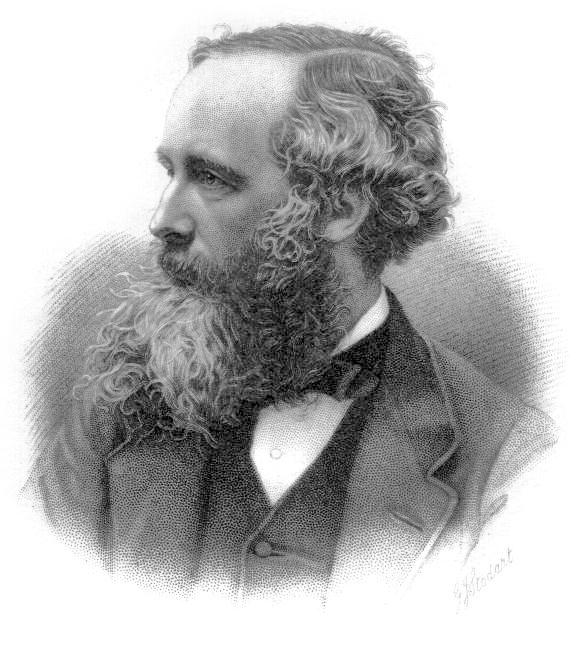
\includegraphics[width=9cm]{archivos/maxwell}
        \caption{James Clerk Maxwell (1831 - 1879) \cite{Maxwell} }
        \label{fig:maxwell}
\end{figure}

\section{Teoría de ondas y señales}
\par Como se mencionó anteriormente, en el proceso de comunicación en el ámbito de las telecomunicaciones la información se envía en forma de señales. Se consideran las señales como un conjunto de impulsos electromagnéticos transmitidos por un emisor y codificados de una manera determinada para que el o los receptores a los que vaya dirigido puedan procesar la información contenida en una señal o conjunto de ellas. Esta información transmitida en forma de señales es el mensaje.
\\
\par Una señal electromagnética se caracteriza por el hecho de variar su intensidad en el dominio temporal. El ejemplo más básico lo encontramos en la onda Seno o Coseno de la figura
\ref{fig:seno}. De esta señal es posible obtener tres parámetros básicos imprescindibles para describir cualquier señal: Amplitud, frecuencia y fase. Se define la amplitud como la variación máxima respecto a un origen determinado y es medido en una magnitud física concreta, en el caso mencionado, la amplitud sería de una unidad, pudiendo ser esta voltios o vatios entre otros. Al tratarse de una señal oscilante aparece el concepto de frecuencia como el número de veces que la señal vuelve a su origen en un tiempo determinado de 1 segundo, la unidad de medida de este parámetro es el \textit{hertzio} (\textbf{Hz}), para el caso mencionado, la frecuencia de la onda es de 1 Hz, puesto que en un segundo la onda realiza un ciclo completo. Finalmente, se denomina fase al concepto de adelanto o retraso de la onda en el dominio temporal con respecto a un origen determinado, normalmente es representado mediante el símbolo \textit{phi} (\textbf{Φ}) y es medido en grados o radianes según sea conveniente, para el caso mencionado la fase sería 0º, puesto que se conoce que una onda seno tiene origen en este valor y no se aprecia ningún adelanto o retraso en la onda mencionada con respecto a este. 
\\
\par Es posible agrupar estos parámetros en forma de ecuación analítica para el caso de una onda simple sin perdidas físicas ni amortiguación y con un movimiento armónico simple como:

\begin{equation}
	x(t)=A\cdot \sin(2\cdot\pi\cdot f+\phi )
	\label{eq: seno}
\end{equation}

\begin{figure}[h]
    \centering
        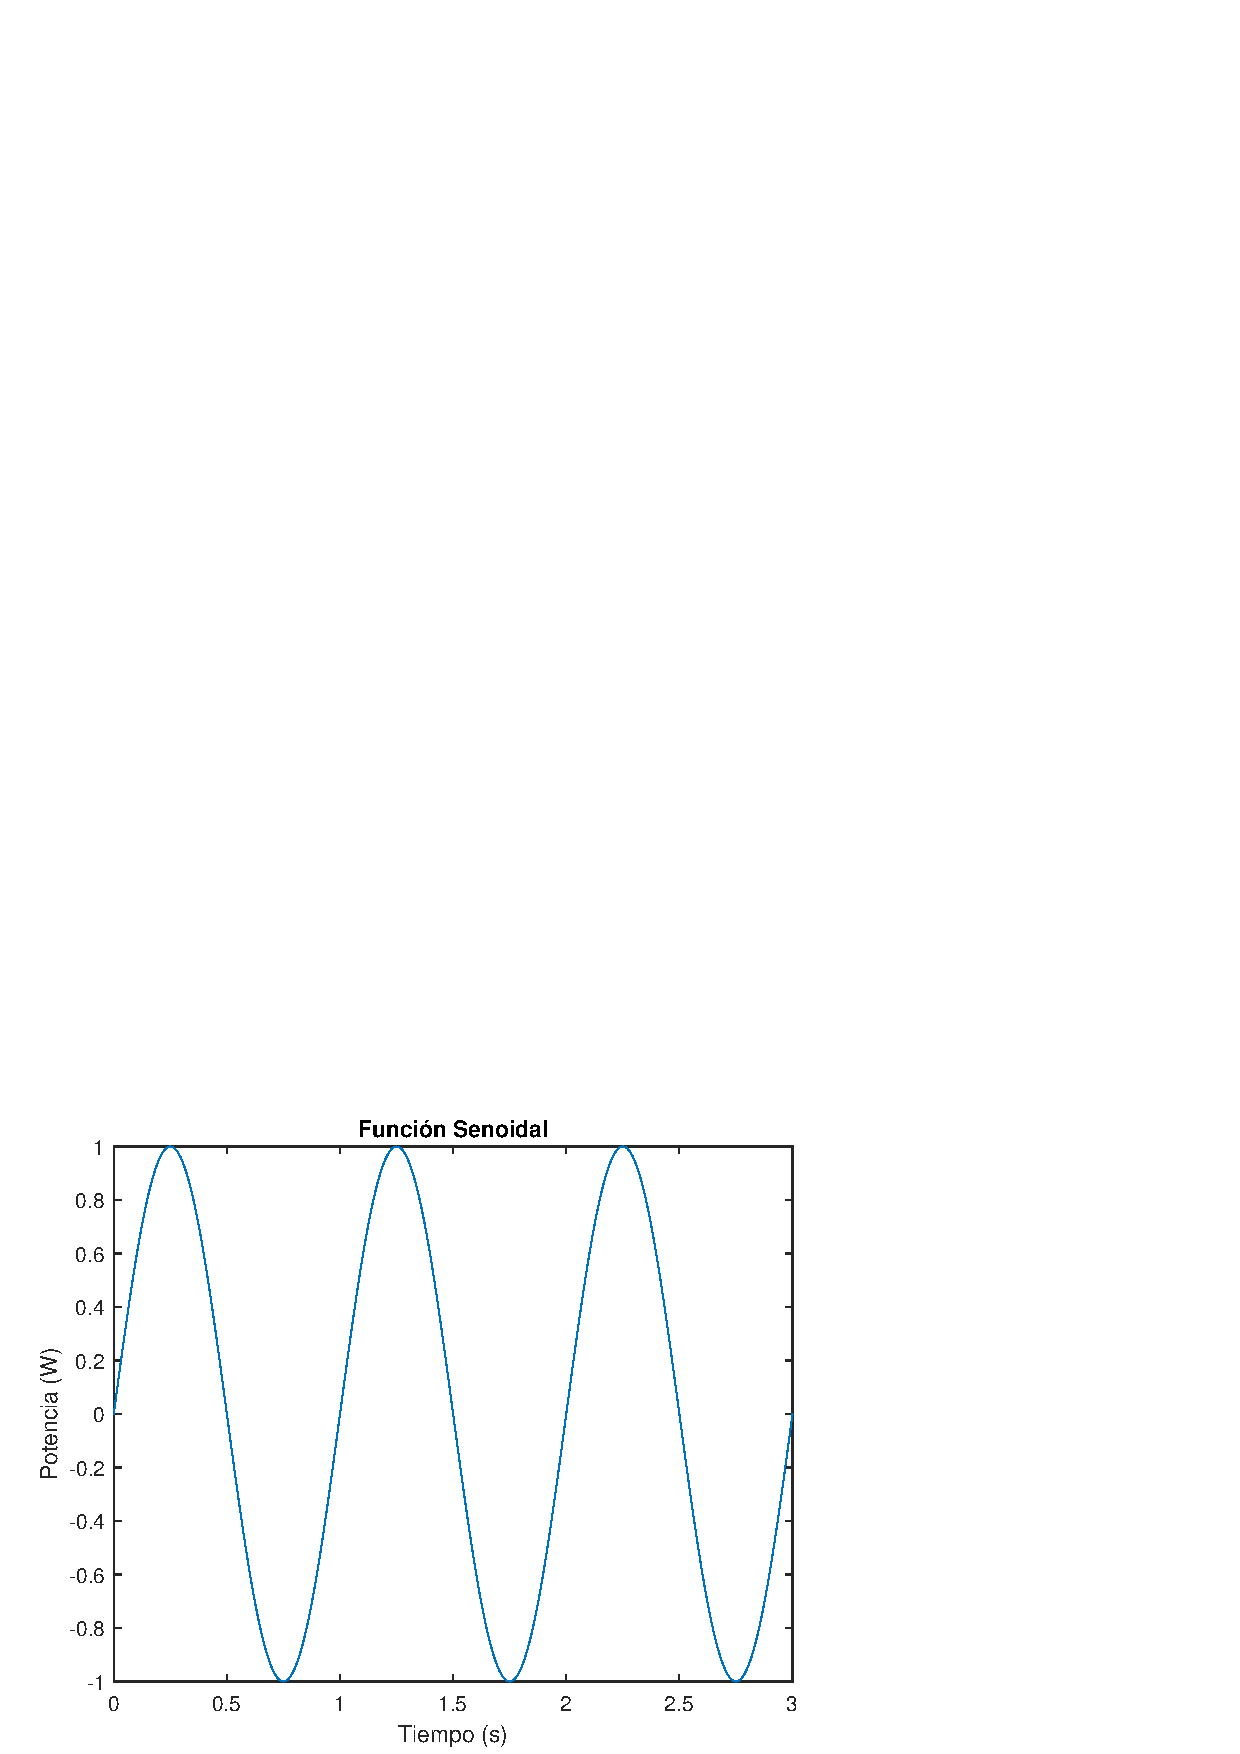
\includegraphics[width=15cm]{archivos/seno}
        \caption{Ejemplo de funcion senoidal}
        \label{fig:seno}
\end{figure}

\par A partir de los parámetros básicos de las ondas es posible el desarrollo de otros parámetros alternativos que facilitan su comprensión y análisis como son: La longitud de onda, definida como la distancia entre los picos o valles de una onda o el periodo, definido como el tiempo que tarda una onda en recorrer un ciclo completo. Estos dos nuevos parámetros se representan en las ecuaciones \ref{ecu:wavelength} y \ref{ecu:periodo} donde \textit{c} es la velocidad de la onda y \textit{f} la frecuencia de esta.

\begin{subequations}
	\begin{eqnarray}
		\lambda &=& \frac{c}{f} \label{ecu:wavelength} \\ % Salto de línea
		T &=& \frac{1}{f} \label{ecu:periodo}
	\end{eqnarray}
\end{subequations}

\par Pero ondas como la que se hacen referencia en la figura \ref{fig:seno}, cuyo tipo de movimiento es el movimiento armónico simple, no reflejan la realidad y la complejidad de las ondas reales que se usarán para la transmisión de información mediante ondas electromagnéticas. Otros conceptos como la atenuación o la amortiguación han de ser tomados en cuenta para describir con mayor precisión el comportamiento de las ondas en medios de transmisión reales como el aire. Si nos centramos en las \gls{oem}, encargadas de transportar los mensajes en forma de energía electromagnética, encontramos que el medio en el que se propagan, no tiene \todo{porque por qué} ser necesariamente el aire, ya que estas se pueden propagar en el vacío. En este medio, las \gls{oem} se propagarán a una velocidad de 300 000 000 m/s, o más conocida como la velocidad de la luz, ya que la luz en sí es una onda electromagnética. 
\\
\par Cuando analizamos un conjunto de partículas subatómicas (electrones o protones) se puede comprobar como a sus alrededores se producen campos eléctricos debido a la interacción entre estos, de repulsión o atracción. A su vez, esta interacción en forma de movimiento de las partículas, produce un campo magnético sobre estas. Es entonces donde, la suma de ambos campos debido a las interacciones entre partículas producen campos electromagnéticos, medio donde se propagaran las \gls{oem}.
\\
\par Las \gls{oem} poseen ciertas características que las describen como son su velocidad de fase y grupo, no teniendo por qué  ser iguales, ni a su vez iguales a la velocidad de propagación en el vacío. Su vector de propagación, el cual apunta la dirección en la que se dirige una onda y cuya magnitud es el número de onda. O su polarización, propiedad que aparecen en las ondas transversales como es el caso de las electromagnéticas. Por convención, cuando se habla de polarización de una \gls{oem} nos referimos a la dirección del campo eléctrico. Existen tres tipos de polarizaciones principales: Lineal, circular y elíptica, y es importante remarcar que a lo largo de este estudio todas las antenas a analizar y estudiar serán diseñadas para trabajar con polarización lineal, si una \gls{oem} de una polarización distinta a la acordada intentara resonar en nuestra antena esta no llegaría a ser captada correctamente y la atenuación producida no permitiría una posible de codificación de esta.

\begin{figure}[h]
    \centering
        \includegraphics[width=15cm]{archivos/oem}
        \caption{Representación esquemática de una Onda Electromagnética}
        \label{fig:oem}
\end{figure}

\par Hasta el momento solo se ha mencionado las señales como mensajes codificados en \gls{oem} que varían en el dominio temporal, pero gracias al matemático \textit{Joseph Fourier} (1768 - 1830), se pudo empezar a estudiar las ondas desde otro dominio: La frecuencia. Fourier desarrolló una serie de transformaciones matemáticas capaces de convertir las expresiones analíticas descritas en un dominio temporal a un dominio frecuencial y viceversa, a las que se denominaron como: \textit{Transformadas de Fourier}, basadas en el \textit{Teorema de Fourier} el cual señala que cualquier señal periódica puede descomponerse mediante una suma infinita de funciones de tipo sinusoidal ponderadas de forma determinada en amplitud y fase y cuyas frecuencias estén relacionadas armónicamente con la frecuencia fundamental de la onda a analizar. 
\\
\par Gracias a la Transformada de Fourier podemos analizar y sintetizar cualquier onda independientemente de su naturaleza física o matemática, y aunque no será usada como tal a lo largo de este trabajo, se hace necesario remarcar la importancia de este desarrollo matemático y la imprescindible contribución hacia el desarrollo de áreas como la acústica o las telecomunicaciones ya que todo avance realizado en esta materia tiene intrínseca la participación de la Transformada de Fourier, como es en nuestro caso, en el que toda representación de señales se realizará en el dominio frecuencial. 
\\
\par Para terminar con el proceso de intercambio de información se hace indispensable mencionar al medio el cual puede tener dos naturalezas: Guiado o radiado. El medio guiado o alámbrico es aquel que depende de una superficie conductora para transmitir la información, por lo general, un cable con propiedades conductoras como cobre u oro, pero también entran en esta categoría la fibra óptica, que transmite por sus filamentos los mensajes codificados en impulsos de luz.  
\\
\par Por otro lado tenemos el medio radiado o también denominado inalámbrico o no guiado, cuyo medio de transporte son los campos electromagnéticos. En este medio no es posible observar las ondas viajar por el espacio, exceptuando el rango de frecuencias correspondiente a la luz visible dentro del espectro electromagnético. Una de las principales propiedades de este medio es que las ondas que viajan a distinta frecuencia son inmunes entre sí a interferirse, lo que permite que los mensajes lleguen del emisor al receptor sin apenas haber sido afectadas en su trayecto por otros mensajes viajando por el campo electromagnético. A partir de ahora el papel del emisor y receptor será tomado por las antenas, las cuales serán capaces de enviar o recibir señales transmitidas en el campo electromagnético en una o varias frecuencias o longitudes de onda. Es por esto que las antenas quedan ahora como los elementos claves para la transmisión de información inalámbrica. 
\\ 
\par En la actualidad existen varios tipos de antena, como estudiaremos más detenidamente en el \todo{tema 3?} y cada uno de ellas se adaptará más específicamente a nuestras necesidades de directividad, ganancia, ancho de banda o eficiencia entre otros. En el estudio que nos ocupa, se diseñará un array de parches en tecnología microstrip que será capaz de trabajar a las frecuencias especificadas para la \gls{5g} de comunicaciones móviles por el \gls{3gpp}.

\section{Las comunicaciones móviles}
\subsection{Las primeras generaciones de telefonía}
\par Las comunicaciones inalámbricas han supuesto una revolución desde su aparición a finales del S.XX hasta la actualidad. El avance de la tecnología, la miniaturización de los componentes, la necesidad de comunicación internacional e incluso las competencias económicas han sido factores claves en la evolución de las comunicaciones móviles. Al hablar de comunicaciones móviles se incluyen en su espectro desde aquellas primeras comunicaciones analógicas como el \textit{Walkie Talkie} o la \gls{1g} hasta los métodos actuales más avanzados como la \gls{4glte}, comunicaciones vía satélite o \gls{voip}. Si se estrecha el círculo al ámbito de la telefonía móvil se puede observar como desde los años 80 distintos estándares de comunicaciones móviles han sido adoptados de la mano de la tecnología disponible en la época e incluso obligando a esta a mejorar para conseguir unos mejores resultados sobre el estándar. 
\\
\par El \gls{1g} fue el primer estándar de telefonía móvil. Fue lanzado en 1979 por la \gls{ntt} en Japón, donde rápidamente se extendió su uso desde su comienzo en el área metropolitana de Tokyo hasta cubrir por completo el área de la isla. Dos años más tarde en 1981 la \gls{nmt} empezó a desplegar esta red en países como Finlandia, Dinamarca o Noruega y más tarde extendiéndose hasta Rusia bajo su propio estándar. En Estados Unidos y Australia esta generación se desplegó bajo el estándar \gls{amps} desarrollado por Motorola y en Reino Unido como \gls{tacs}. En España la \gls{ctne} actualmente conocida como Telefónica, desplegó, bajo el servicio MoviLine, su oferta de \gls{1g} mediante el estándar ETACS, una actualización del sistema \gls{tacs} que incluía una nueva banda de frecuencias. Esta primera generación de telefonía móvil se basaba en el uso de la electrónica sólo en los servicios de red de acceso, ya que el resto de la red de comunicación se sostenía sobre la red analógica de telefonía ya existente en cada país, con lo que solo se permitía el tráfico de voz sobre ella.

\begin{figure}[h]
    \centering
        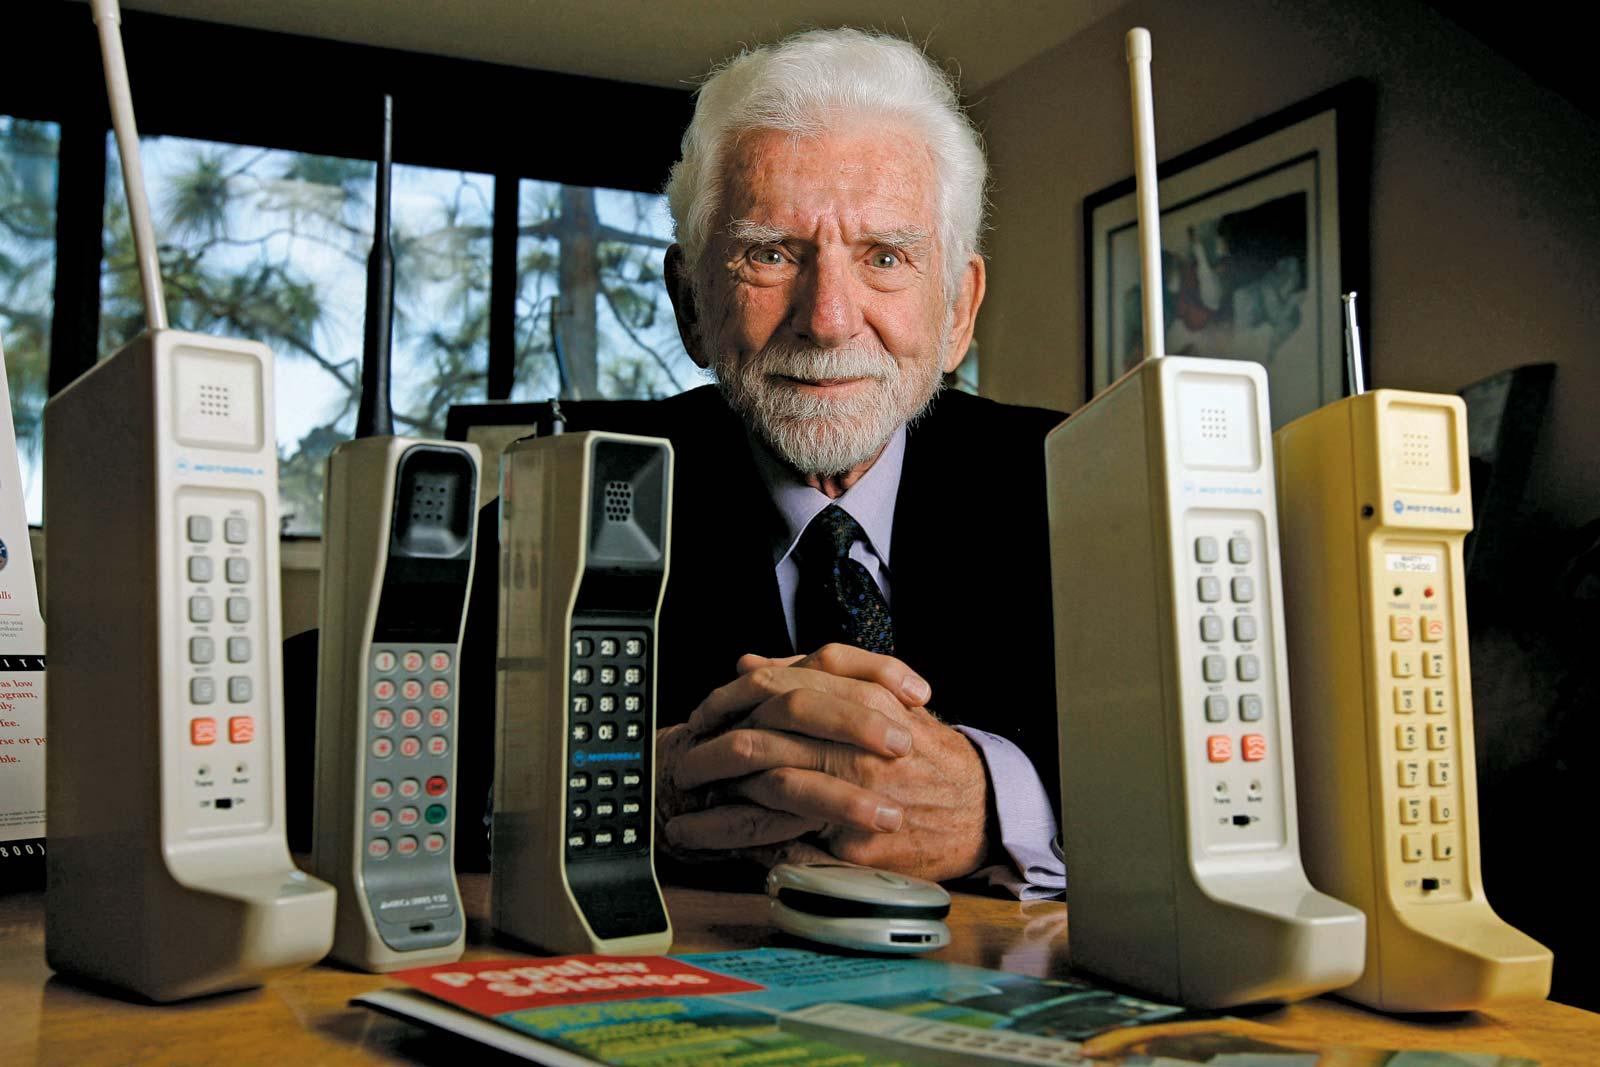
\includegraphics[width=15cm]{archivos/motorola}
        \caption{Martin Cooper (Motorola) junto a teléfonos móviles de primera generación}
        \label{fig:motorola}
\end{figure}

\par Tras una década, en el 1992, apareció el siguiente estándar de telefonía fue la \gls{2g}, donde se adoptaron sistemas digitales tanto en la red de acceso o \gls{ran}, como en el Core, es decir la parte central de la red de telecomunicaciones donde, entre otras funcionalidades, se enruta el tráfico.
El estándar asociado al \gls{2g} fue el denominado \gls{gsm}, este era capaz de, además de realizar llamadas, ahora si sobre la red digital, la transmisión de paquetes de datos, lo que permitió el uso de mensajería instantánea con el SMS o las primeras conexiones a Internet móvil, aun más consolidado con la evolución del estándar \gls{gsm}: el \gls{gprs}, que conseguía throughputs, o tasas de transmisión efectivas de hasta 230 Kbps en su último release (EDGE), también conocido como el 2.5G. Esta generación de telefonía móvil se desplegó sobre las bandas de 900 y 1800 Mhz. En España, tras la desaparición del servicio MoviLine, apareció Movistar, también bajo el mando de Telefónica, con el primer despliegue de red digital móvil. Tras la liberación del mercado de las telecomunicaciones, otras operadoras como Aritel (Vodafone) o Amena (Orange) empezaron a ofrecer sus servicios móviles a nivel nacional. 
\\
\par Otra de las novedades del estándar \gls{2g} fue la incursión de la denominada Tarjeta SIM, la cual permitía identificar a cada suscriptor. En su interior era capaz de almacenar la información sobre la suscripción del usuario, un directorio telefónico o los parámetros de la red a la que se debía conectar según la operadora. Actualmente la mayoría de países que adoptaron esta tecnología están en proceso de desconexión de sus estaciones bases \gls{2g} puesto que se considera un estándar ya obsoleto y su uso ha quedado restringido a ciertas zonas donde las operadoras no consideraron conveniente el despliegue de nuevas redes de telefonía como en zonas rurales o carreteras.
\subsection{La tercera generación}
\par A principios de este siglo, la \gls{3g} de telefonía fue lanzada por la \gls{itu} bajo el nombre de IMT-2000. A esta generación de telefonía también se le denominó \gls{umts}, y es que es el primer estándar que aseguraba compatibilidad telefónica entre países ya que el consorcio encargado de velar por el correcto uso del estándar, la \gls{3gpp}, estaba formado por empresas tecnológicas internacionales como \gls{att}, Ericsson, Motorola o \gls{ntt}. Este nuevo servicio de telefonía permitía conectividades de hasta 20 Mbps en su banda de 2100 MHz, lo que permitió la proliferación de los \textit{smartphones}, donde ahora ya era posible acceder fácilmente a Internet, el correo electrónico u otros servicios multimedia online. 
\\
\par El \gls{3g} implementaba un nuevo tipo de modulación denominada \gls{wcdma}, el cual permitía una mayor eficiencia espectral debido a que todos los usuarios eran capaces de transmitir simultáneamente, pero separados mediante códigos de identificación únicos. Para separar la señal en el medio de transmisión cada bit era multiplicado por el código de identificación de cada usuario. Conforme pasaron los años, nuevos sub-estándares fueron lanzados mejorando las especificaciones iniciales del \gls{3g}, como el \gls{hspa}, que permitía tasas de transmisión de hasta 42 Mbps y 168 Mbps en HSPA+ e introducía por primera vez los conceptos de \gls{mimo} y beamforming que se explicarán más adelante.
\subsection{Actualidad, la cuarta generación}
\par Finalmente, en el año 2013 se lanzó oficialmente el \gls{4glte}, desarrollado también por el \gls{3gpp}. El término LTE, en español, "evolución a largo plazo" es adoptado para este estándar puesto que realmente esta generación no añade una arquitectura nueva al sistema sino que se basa en las arquitecturas ya consolidades del \gls {3g} y el \gls{2g}. Es por esto que la \gls{itu} no consideró que el LTE desplegado actualmente sea una completa nueva generación, en este caso \gls{4g}. Las principales características del \gls{lte} son un incremento de las tasas de transmisión, una mayor eficiencia energética y seguridad, una menor latencia, y más fácil de desplegar por los operadores.
\\
\par Con el \gls{lte} se han llegado a conseguir tasas de hasta 173 Mbps de bajada, y con la implementación de \gls{mimo} con 4 antenas en los dispositivos, esta se duplicaba hasta los 300 Mbps. Además, en este nuevo estándar, sólo se utiliza la conmutación de paquetes, es decir, se descartaban por completo en el core de la red, los antiguos sistemas de conmutación de circuitos para transferir las llamadas. La modulación escogida para el \gls{lte} fue la \gls{ofdm}, la cual transporta la información modulada en \gls{qam} pero multiplexado en un conjunto de diferentes portadoras, lo que permite una mayor eficiencia espectral con respecto al \gls{3g}.
\subsection{El futuro, la quinta generación}
\par El \gls{5g} es el nuevo estándar de telefonía móvil, sucesora de la \gls{4g}, llevado a cabo por el \gls{3gpp} en su Release 15 y 16. Este nuevo estándar de telefonía permitirá:
\begin{itemize}
\item Conexiones con throughputs, o tasas de transmisión efectivas de hasta 10 Gbps, es decir, hasta 10 veces más rápido que el \gls{4g}.
\item La latencia, definida como la suma de retrasos temporales producidas en un sistema de comunicación debido a la velocidad de propagación limitada, perdidas, etc. se reducirán hasta valores de 1 ms en comparación con el rango de entre 30 y 50 ms que obtenemos en redes \gls{4g} y \gls{wifi}
\item Capacidad de conexiones masivas para dispositivos \gls{iot} lo que permitirá  el desarrollo de redes de comunicación \gls{m2m} aumentando la eficiencia energética de estas, así como su disponibilidad y seguridad, lo que será imprescindible para tecnologías emergentes como la conducción autónoma o las Smart Cities, es decir, el proceso de uso de las \gls{tic} para modernizar el entorno urbano ofreciendo servicios de mejora del transporte público, seguridad ciudadana, ahorro energético, etc.
\item Mejora de la diversidad en recepción con respecto al \gls{4g} mediante el uso del \gls{mimo} Masivo. Esta tecnología aprovecha el uso de múltiples antenas sobre un mismo dispositivo para usarlas como enlaces independientes, de forma que la velocidad de conexión pueda aumentar de forma significativa. Con \gls{mmimo} se dispondrán de decenas de antenas por dispositivo para hacer que la conexión sea más rápida y eficiente.
\item El uso del beamforming, proceso por el cual se direcciona el haz de emisión de la antena y mediante técnicas de procesado digital se calcula en qué dirección se hará más eficiente la comunicación entre la antena y el dispositivo además de poder hacer cálculos sobre ruido e interferencias para mejorar la eficiencia de la antena.
\end{itemize}

\par Además, el \gls{5g} emitirá sobre nuevas bandas de frecuencia, las cuales categorizaremos como \textit{Bandas Sub-6Ghz} y \textit{Bandas Super-6Ghz}. En el caso del plan nacional para el 5G aprobado por el \gls{minetur}, principal responsable de la gestión de los temas referentes a telecomunicaciones a nivel estatal en España, las bandas de frecuencias aprobadas para el 5G son:
\begin{itemize}
\item\textbf{700 Mhz:} Esta banda antes usada para la retransmisión de la \gls{tdt} y adjudicada para su uso en el \gls{5g} mediante el segundo dividendo digital será clave para la retransmisión de señales móviles \gls{5g} que necesitan alcanzar los interiores de los hogares y las oficinas puesto que su mayor longitud de onda con respecto a otras bandas la hace apta para penetrar o difractar sobre muros.
\item\textbf{3.4-3.8 Ghz: }Estas bandas de frecuencias eran anteriormente usadas para radioenlaces de transporte de señal de televisión, actualmente en desuso. Permitirán mayores tasas de velocidad con respecto a los 700 Mhz, pero su atenuación será mayor, lo que la hace adecuada para transmisión en zonas urbanas o carreteras.
\item\textbf{26 Ghz: }En este rango de frecuencias entramos en las denominadas como \gls{mmwv} es decir, ondas cuya longitud de onda esté en el orden de milímetros. Esta banda de frecuencia presume de tener mayor disponibilidad en cuanto a ancho de banda lo que permitirá conexiones de banda ancha ultrarápidas.
\end{itemize}

\par Como se puede, la tendencia futura en cuanto a comunicaciones móviles de alta velocidad va de la mano y es directamente proporcional a la frecuencia a la que se emita la señal, pero a su vez, este incremento de frecuencia hace más vulnerables a las transmisiones de ser interferidas o atenuadas durante su retransmisión, lo que haría muy difícil el uso de las redes \gls{5g} cuando la antena se sitúa en el exterior y los dispositivos en interiores. En este escenario surge el concepto, ya existente en el \gls{4g} del uso de Small Cells. Las Small Cells son pequeñas estaciones base que se sitúan en puntos estratégicos tanto en interiores como oficinas o centros comerciales, como en exteriores en sitios con una gran afluencia de personas y por ende, de dispositivos móviles. 

\par En el \gls{5g}, el concepto de Small Cell (fig. \ref{fig:stadika}) es imprescindible. Debido al crecimiento exponencial del uso de dispositivos por parte de usuarios y empresas cada vez se hará más difícil el hecho de que una sola estación base pueda dar cobertura y una tasa de transmisión aceptables al estándar a estos dispositivos. Es por ello que en los nuevos despliegues de \gls{5g} las operadoras se inclinarán más por el uso de muchas Small Cells a lo largo de la ciudad que den servicio a los usuarios de un rango muy limitado de espacio, pero con muy buena cobertura y tasas de transmisión, que a la instalación de estaciones base convencionales que dan cobertura en radios muy amplios de distancia, lo que en grandes urbes puede suponer la saturación de la propia estación base.

\begin{figure}[h]
    \centering
        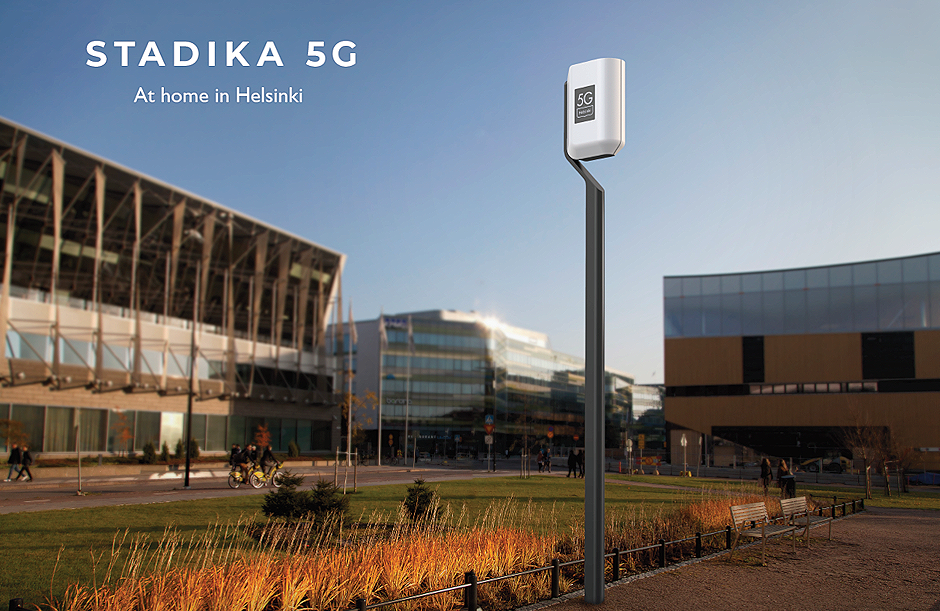
\includegraphics[width=15cm]{archivos/stadika}
        \caption{Stadika: Concepto de diseño de Small Cells 5G para la ciudad de Helsinki}
        \label{fig:stadika}
\end{figure}

\par Bajo todo este nuevo escenario de comunicaciones avanzadas que plantea para un futuro muy cercano se han de plantear qué tecnologías se usarán para cubrir las metas y especificaciones marcadas de la manera más robusta y eficiente. El \gls{5g} tendrá una completa dependencia de los sistemas informáticos diseñados para alcanzar estas metas, mediante técnicas de procesado digital y nuevos algoritmos podremos ir añadiendo características e incluso mejorando las ya existentes sin necesidad de alterar todo el sistema ya instalado en la red.

\section{Motivación}
\par Ante todo este nuevo escenario de tecnología móvil que se plantea para los próximos años cabe la necesidad de adaptar la tecnología existente para ser compatible con las nuevas especificaciones. En el fondo la pieza clave de toda comunicación inalámbrica digital es la antena, y es importante que un correcto diseño de esta para asegurar que los parámetros de funcionamiento de están aseguren una correcta adaptación al estándar. 
\\
\par Las antenas de parche de tipo microstrip llevan siendo usadas durante décadas para la transmisión de información entre dispositivos móviles y las estaciones base, así como en comunicaciones aéreas, satelitales, o aeroespaciales, debido a la flexibilidad respecto a su tamaño, peso, coste, rendimiento e incluso facilidad de instalación. En este proyecto se diseñarán y analizaran una serie de arrays o conjunto de antenas, que nos permitirán mejorar ciertas características del sistema, para trabajar a las frecuencias de 2.4, 6, e incluso 27 Ghz, bandas usadas en las comunicaciones \gls{wifi} actuales y que se prevén usar en comunicaciones \gls{5g} en el futuro. 


\section{Estructura del proyecto y metodología}
\label{sec:medodologia}
\par Este proyecto estará dividido en dos partes fundamentales, un marco teórico, donde se realizará una completo resumen sobre los conceptos básicos de las líneas de transmisión: Adaptación e impedancias, tecnología microstrip en líneas de transmisión, etc. Antenas: Tipos de antena, parámetros de estudio básicos, etc. Y en un marco más específico, sobre las antenas de tipo parche en tecnología microstrip: Métodos de alimentación, componentes, tipos, análisis, etc. Finalmente se expondrá la parte de experimentación, donde se estudiarán y analizarán los diseños de distintos tipos de configuraciones de arrays para antenas de tipo parche con tecnología microstrip.
\\
\par Para realizar la parte experimental del proyecto se hará uso del software de análisis electromagnético 3D: Ansys\textregistered HFSS (High Frequency Structure Simulator). Este software es usado para diseñar y simular componentes electrónicos de alta frecuencia como antenas, arrays, filtros o placas de circuito impreso. Con el, se diseñarán las configuraciones de antenas especificadas y se simularan sus efectos electromagnéticos como si se tratara de una cámara anecóica, para finalmente poder analizar los resultados obtenidos y los valores de los parámetros característicos de la antena así como comprobar la viabilidad del producto final en términos de rendimiento o dimensiones.
\\
\par Por otro lado, se hará uso de la herramienta de cálculo matemático MathWorks\textregistered MATLAB, con la que realizaremos cálculos básicos sobre las dimensiones de la antena a diseñar en función a los parámetros de construcción de esta.
	% Plantilla: Se muestran contenidos
%%%%%%%%%%%%%%%%%%%%%%%%%%%%%%%%%%%%%%%%%%%%%%%%%%%%%%%%%%%%%%%%%%%%%%%%
% Plantilla TFG/TFM
% Escuela Politécnica Superior de la Universidad de Alicante
% Realizado por: Jose Manuel Requena Plens
% Contacto: info@jmrplens.com / Telegram:@jmrplens
%%%%%%%%%%%%%%%%%%%%%%%%%%%%%%%%%%%%%%%%%%%%%%%%%%%%%%%%%%%%%%%%%%%%%%%%

\chapter{Teoría de Antenas}
\par En este capitulo se realizará una breve contextualización sobre el concepto de antena así como un repaso a los parámetros que las caracterizan. Estos conceptos son, por lo general, aplicables a cualquier tipo de antena, en capítulos posteriores se especificará lo aprendido para el caso de las antenas en tecnología microstrip.

\section{Conceptos básicos}

\par Las antenas son transductores entre un medio guaiado y uno radiado. En su diseño más simplificado se analizaría un conductor metálico por el cual fluye una corriente variable en el tiempo. Se entiende como medio guiado a cualquier tipo de línea de transmisión: Cable coaxial, fibra óptica así como guías de onda. Y como medio radiado el aire o el espacio. Las antenas transmisoras serán las encargadas de transformar esta las corrientes eléctricas a \gls{oem}, mientras que las receptoras tomarán las \gls{oem} desde el medio radiado y las convertirán de nuevo a impulsos eléctricos para su posterior procesado. Las primeras antenas fueron diseñadas en 1888 por \textit{Heinrich Hertz} pero no fue hasta 1895 cuando \textit{Guglielmo Marconi} empezó a desarrollar antenas con el objetivo de transmitir información a largas distancias.
\\
\par Como se explico en el \todo{capitulo1}, cualquier variación de un campo eléctrico generará un campo magnético y viceversa. Cuando ambos campos conviven y existen variaciones de estos campos se dice que existe una radiación electromagnética. Para entender el principio de funcionamiento de una antena se tomará como ejemplo el caso de hilo conductor cerrado. Si se introdujera una corriente eléctrica fluctuante en el tiempo dentro del conductor, por el principio de inducción electromagnética (Tercera ecuación de Maxwell, Ley de Faraday-Lentz) se produciría un campo magnético fluctuante y un campo eléctrico asociado a su alrededor, estaríamos hablando de un campo electromagnético. Pero este campo electromagnético no se propagaría y estaría siempre al rededor del conductor cerrado. Para poder propagar las \gls{oem} se debe conseguir separar la onda electromagnética del conductor.
\\
\par Para entender el efecto de separación se tomará como referencia dos cargas eléctricas de distintas polaridades separadas a una distancia determinada (fig. \ref{fig:campo1}), a esto se le conoce como dipolo eléctrico y producirán un campo eléctrico cuyas líneas de fuerza irán del positivo al negativo. Estás dos cargas intentarán juntarse debido al efecto de atracción. En el momento de mayor separación de las cargas, su velocidad será nula y su aceleración máxima. Conforme se vayan acercando la velocidad irá aumentando y la aceleración disminuyendo hasta que en el punto donde se encuentran la velocidad será máxima y la aceleración nula. Suponiendo un escenario teórico sin pérdidas estás cargas estarían fluctuando e intercambiando sus posiciones indefinidamente. Si se analiza el campo eléctrico producido por las cargas mientras estas están fluctuando se observaría como, en vez de seguir encontrando un campo eléctrico simple de menor intensidad, este se deforma debido a la aceleración presente en las cargas. Esta deformación es también conocida como efecto \textit{kink} (fig. \ref{fig:campo2}).
\\
\par Continuando con el experimento se observa como pasado un lapso de un 1/4 del periodo de la oscilación, momento en el que las dos cargas se cruzan en el mismo punto, el campo eléctrico producido es nulo, cerrándose así las líneas de campo que habían sido producidas cuando las partículas estaban aún separadas (fig. \ref{fig:campo3}). Es entonces cuando se produce la propagación y generación del frente de onda del campo eléctrico, con su respectivo campo magnético asociado. Se debe observar como la longitud de la \gls{oem} propagada es exactamente el doble de la longitud existente entre las dos cargas (fig. \ref{fig:campo4}).\\

\begin{figure}[h]
\centering
	\begin{subfigure}[b]{0.3\textwidth} % Espacio horizontal ocupado por la subfigura
		\centering
		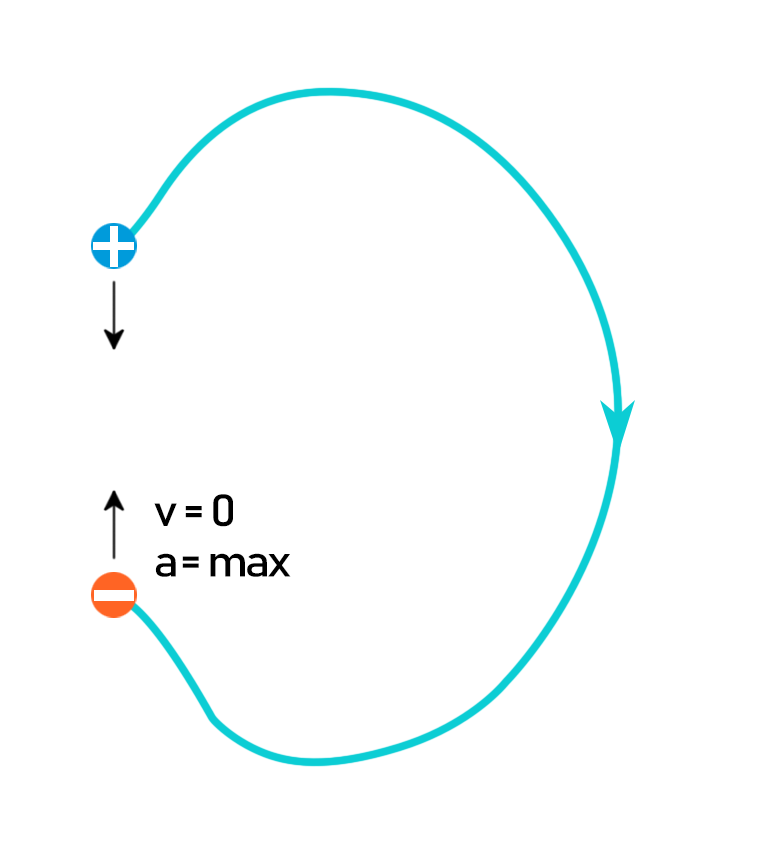
\includegraphics[width=5cm]{archivos/campos/campos1} % Tamaño de la imagen
		\caption{t = 0}
		\label{fig:campo1}
	\end{subfigure}
~ % Añadir el espacio deseado, si se deja la linea en blanco la siguiente subfigura ira en una nueva linea
	\begin{subfigure}[b]{0.3\textwidth} % Espacio horizontal ocupado por la subfigura
	\centering
		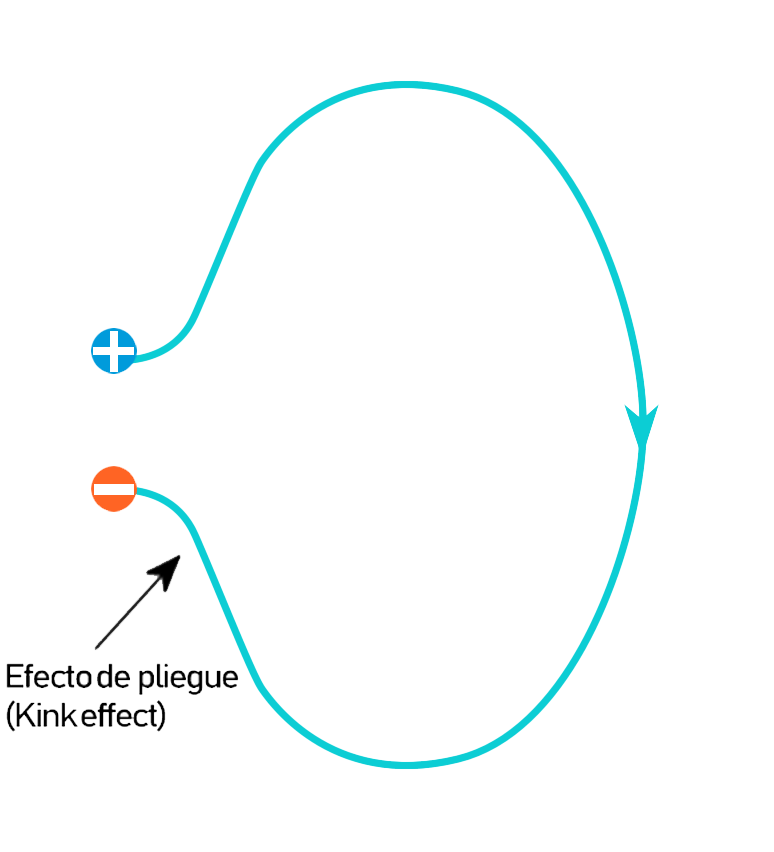
\includegraphics[width=5cm]{archivos/campos/campos2} % Tamaño de la imagen
		\caption{0 < t < T/4}
		\label{fig:campo2}
	\end{subfigure}
	\begin{subfigure}[b]{0.3\textwidth} % Espacio horizontal ocupado por la subfigura
	\centering
		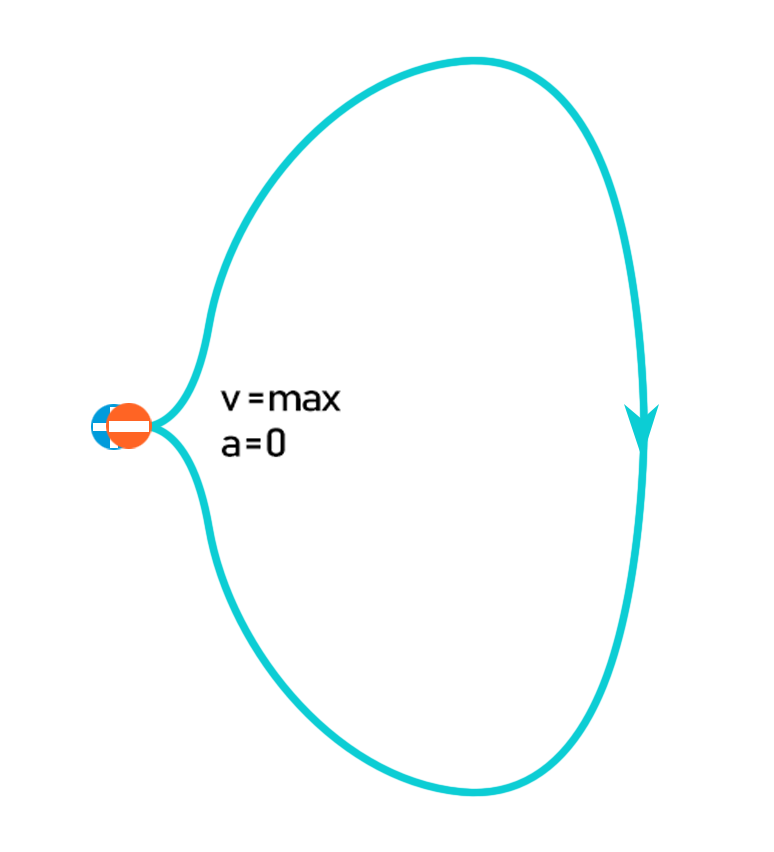
\includegraphics[width=5cm]{archivos/campos/campos3} % Tamaño de la imagen
		\caption{t = T/4}
		\label{fig:campo3}
	\end{subfigure}
	\begin{subfigure}[h]{0.5\textwidth} % Espacio horizontal ocupado por la subfigura
	\centering
	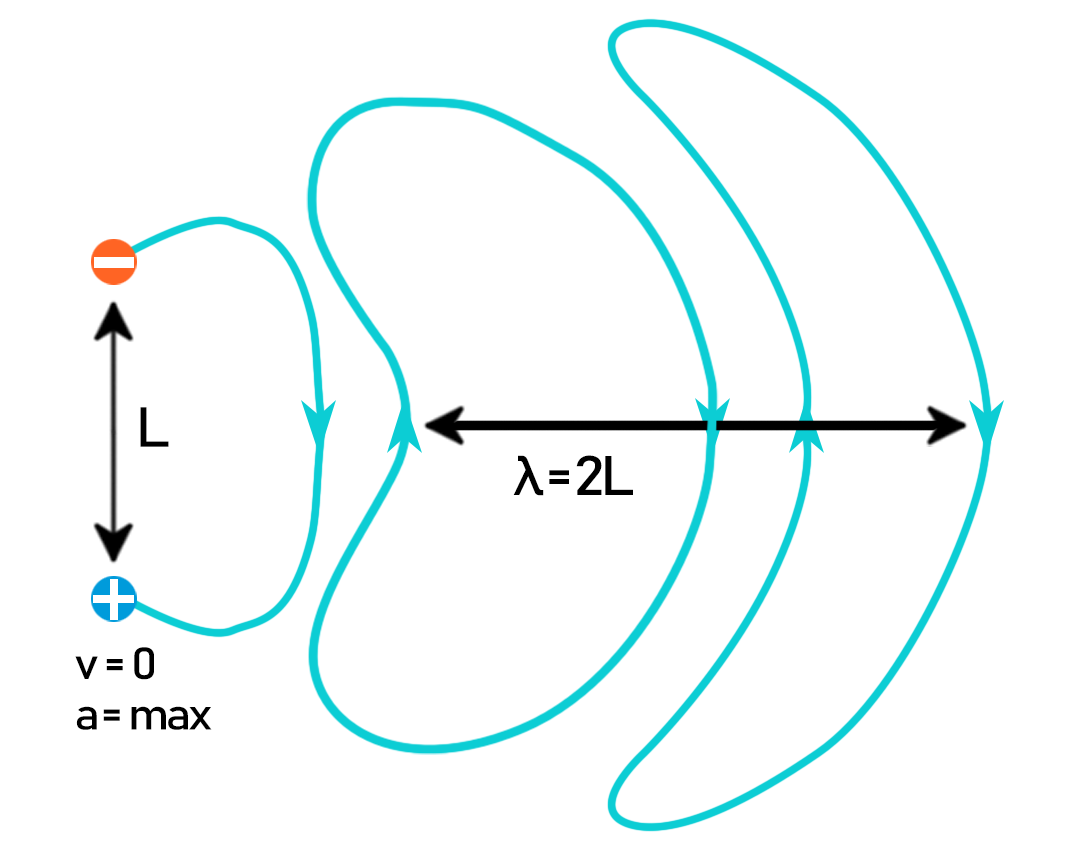
\includegraphics[width=10cm]{archivos/campos/campos4} % Tamaño de la imagen
	\caption{t > T/4}
	\label{fig:campo4}
\end{subfigure}
\caption{Proceso de separación de campo eléctrico}\label{sistemass}
\end{figure}

\par En la práctica se puede simular el experimento en lo que se denomina como antena dipolo, la antena más básica existente, que será estudiada con mayor detenimiento a lo largo de este capítulo. En una antena dipolo, al aplicar una tensión variable sobre los bornes de esta, las cargas irán oscilando de un extremo a otro según la polaridad del generador en ese instante, produciendo campos eléctricos capaces de separarse de la antena, con su consiguiente generación de campos magnéticos. El conjunto de la propagación de ambos campos son los campos electromagnéticos en los que se propagará la \gls{oem}. En la figura \ref{fig:dipolo} se pueden observar ejemplos de antenas dipolo. 

\begin{figure}[h]
\centering
	\begin{subfigure}[b]{0.4\textwidth} % Espacio horizontal ocupado por la subfigura
		\centering
		\includegraphics[width=7cm]{archivos/dipolo/dipole1} % Tamaño de la imagen
		\caption{Esquema de un dipolo}
		\label{fig:dipolo1}
	\end{subfigure}
~ % Añadir el espacio deseado, si se deja la linea en blanco la siguiente subfigura ira en una nueva linea
	\begin{subfigure}[b]{0.4\textwidth} % Espacio horizontal ocupado por la subfigura
	\centering
		\includegraphics[width=7cm]{archivos/dipolo/dipole2} % Tamaño de la imagen
		\caption{Dipolo instalado sobre un poste}
		\label{fig:dipolo2}
	\end{subfigure}
\caption{Antenas dipolo de media onda}\label{fig:dipolo}
\end{figure}

\par El principio básico de diseño de antenas se basa en la geometría de estas. Es importante remarcar que para que la transmisión de la señal aplicada por el generador y que se desea convertir en \gls{oem}, la longitud de los lados del dipolo deben estar relacionados con la longitud de onda de la señal que se desea transmitir. En el caso del dipolo, los extremos tendrán una longitud de $\lambda$/4. Al juntan ambos extremos se puede observar que la antena tendrá una dimensión total de $\lambda$/2, y si se tiene en cuenta que la longitud de onda de la \gls{oem} generada es el doble de la longitud de la antena, se obtendrá una \gls{oem} radiada cuya frecuencia sea idéntica a la aplicada por el generador.
\\
\par Aunque se ha analizado el caso de una antena para que funcione como transmisora, el mismo principio de funcionamiento se aplica cuando queremos que esta funcione como receptora de señales. Una \gls{oem} que viaje por el espacio será capaz de hacer oscilar las cargas de una antena receptora cuando su frecuencia y las longitud de la antena estén directamente relacionadas y se produzca la resonancia sobre esta. La diferencia es que a la salida de la antena receptora no tendremos un generador, sino lo que denominaremos como carga, pudiendo ser esta cualquier tipo de componente eléctrico o electrónico que sea capaz de trabajar con las corrientes eléctricas producidas por la fluctuación de cargas eléctricas en el interior de la antena.

	% Plantilla: Se muestran listas
%%%%%%%%%%%%%%%%%%%%%%%%%%%%%%%%%%%%%%%%%%%%%%%%%%%%%%%%%%%%%%%%%%%%%%%%
% Plantilla TFG/TFM
% Escuela Politécnica Superior de la Universidad de Alicante
% Realizado por: Jose Manuel Requena Plens
% Contacto: info@jmrplens.com / Telegram:@jmrplens
%%%%%%%%%%%%%%%%%%%%%%%%%%%%%%%%%%%%%%%%%%%%%%%%%%%%%%%%%%%%%%%%%%%%%%%%

\chapter{Antenas Microstrip}
\label{antenasmicrostrip}

\section{Introducción}
\par Las antenas de parche o antenas microstrip son un tipo de antenas de tipo planar que utilizan la tecnología microstrip para su funcionamiento. En el año 1953 \textit{G. A. Deschamps} y \textit{W. Sichak} presentaron ante el Tercer Simposio sobre Investigación y Desarrollo de Antenas organizado por las Fuerzas Aéreas de los Estados Unidos su trabajo "Microstrip Microwave Antennas" (Antenas de Microondas Microstrips), lo que se considera como el primer \textit{paper} sobre este tipo de antenas, pero no fue hasta dos décadas más tarde, en 1970 cuando, gracias al desarrollo de los \gls{pcb}, se pudieron empezar a realizar los primeros desarrollos de líneas de transmisión y antenas con tecnología microstrip. Desde entonces, las antenas microstrip se han convertido en uno de los tipos de antena más usado para un alto abanico de aplicaciones. 
\\
\par Entre sus principales ventajas se encuentra su delgadez y capacidad de adaptación a distintos tipos de superficies, incluso pudiendo ser conformadas en superficies curvas y no planares. Además son antenas simples, muy ligeras, fáciles de diseñar, con un coste de producción bajo, fáciles de transportar, y preparadas para ser integradas en arrays. Por estas razones, los circuitos y antenas microstrip son comúnmente usados para la fabricación de circuitos monolíticos integrados para microondas (MMICs) en aplicaciones civiles, militares, gubernamentales y comerciales como identificación por radio frecuencia (RFID), retransmisión de radio, sistemas de comunicaciones móviles, \gls{gps}, televisión, comunicaciones satelitales (fig. \ref{fig:satgalileo}), sistemas de vigilancia, radar, y guiado de misiles entre otros. 
\\
\par Por otra parte, las antenas microstrip son muy versátiles en términos de resonancia y polarización, con obtención de buenos patrones de radiación y fácil adaptación de impedancias. Si además sumamos al circuito elementos adaptativos como diodos varicap, se pueden llegar a diseñar antenas microstrip con frecuencias, impedancias, y patrones de radiación variables. En contra, el uso de antenas microstrip conlleva ciertas limitaciones como su alto factor de calidad (Q), necesidad de limitar la potencia que atraviesa el circuito, baja eficiencia, baja pureza de polarización y ancho de banda limitado. En ciertas aplicaciones, estas limitaciones pueden ser usadas a favor, como el hecho de tener bajos anchos de banda puede ser deseado a la hora de usar las antenas microstrip en aplicaciones de seguridad gubernamental puesto que se limita el rango de penetración externa por parte de posibles atacantes.

\begin{figure}[h]
    \centering
        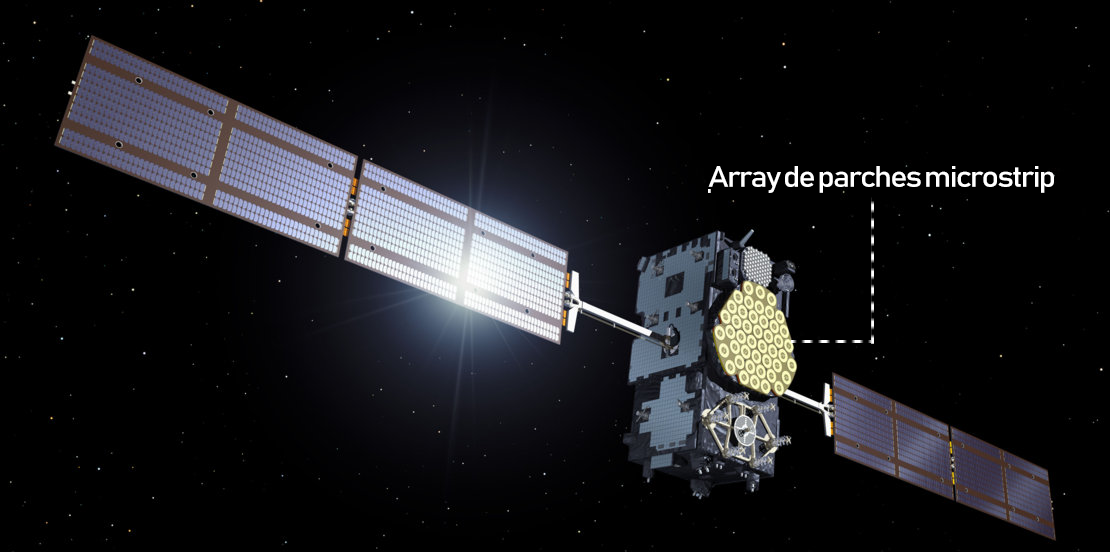
\includegraphics[width=15cm]{archivos/sate}
        \caption{Satélite IOV Galileo}
        \label{fig:satgalileo}
\end{figure}

\section{Características básicas}

\par Las antenas microstrip están formadas por tres elementos básicos: Una capa conductora muy fina, hasta tres órdenes de magnitud menor a la longitud de onda en el espacio de la señal que se desea transmitir por ella, a la que denominaremos como parche. Este arreglo metálico está situado a, aproximadamente, la centésima parte de la longitud de onda en el espacio, del plano de tierra o masa de la antena, que consistirá en una superficie metálica normalmente, del mismo grosor que el parche. Para que un parche rectangular resuene a una frecuencia concreta, la longitud de este debe ser de entre la mitad y un tercio de la longitud de onda de la señal deseada.
\\
\par Entre el parche y el plano de masa se sitúa el dieléctrico o substrato, encargado de aislar ambos materiales previamente mencionados. El substrato se caracteriza por su permitividad relativa o constante dieléctrica ($\epsilon_{r}$), y para la construcción de antenas microstrip, esta suele oscilar entre valores de 2.2 y 12 \todo{unidad}. Cuanto más grueso sea el substrato, mejores resultados respecto a ancho de banda y eficiencia obtendremos en el diseño, sacrificando la pérdida de espacio ocupado por el substrato correspondiente, la cual puede ser muy limitada en ciertas aplicaciones. Por otro lado, substratos finos con valores de permitividad relativa alta son usados para aplicaciones de microondas ya que estas requieren contornos muy finos para evitar radiaciones indeseadas y acoplamientos.
\\
\par Normalmente, las antenas microstrip están integradas en otros circuitos de microondas, con lo que es necesario llegar a un compromiso entre las características de diseño requeridas por la aplicación y el buen rendimiento de la antena. Además de parches rectangulares, las antenas microstrip pueden tomar diversidad de formas para adaptarse a las limitaciones de diseño especificadas por la aplicación. Entre las formas más comunes que toman las antenas microstrip se encuentran cuadrados, circulos, elípses, sectores circulares, triangulos, o dipolos. Diseños específicos como los círculos los normalmente utilizados para conseguir características más específicas como polarización cirucular. Otro método para conseguir este tipo de polarizaciones así como aumentar el ancho de banda o la directividad es el uso de arrays de antenas microstrip. 
\\
\par Las características de sintonización y adaptación de las antenas de parche microstrip residen principalmente en las dimensiones de los elementos que la componen. En la figura \ref{fig:elementos} se puede observar cómo se organiza una antena microstrip de un solo elemento y las denominación común que se le dan a las variables que definen la dimension de estos elementos. Las variables más importantes a la hora de diseñar una antena microstrip rectangular son los siguientes:

\begin{itemize}
\item \textbf{L: }Longitud del parche
\item \textbf{W: }Anchura del parche
\item \textbf{h: }Altura o espesor del dieléctrico
\item \textbf{t: }Altura o espesor del parche y de la tierra
\item \textbf{$\epsilon_{r}$: }Constante dieléctrica
\end{itemize}
 
\begin{figure}[h]
    \centering
        \includegraphics[width=15cm]{archivos/parche/elemento}
        \caption{Partes de una antena microstrip}
        \label{fig:elementos}
\end{figure}

\section{Ondas en antenas microstrip}

\par Durante el proceso de normal funcionamiento de las antenas microstrip, diferentes tipos de ondas pueden aparecer en sus líneas y superficies. Algunas de estas ondas son indeseadas puesto que pueden causar interferencias sobre los campos eléctricos que proceden del generador que nosotros hayamos instalado, y es de vital importancia diseñar la la antena de forma que su aparición sea mínima. Existen cuatro tipos de ondas principales:

\begin{itemize}
\item \textbf{Ondas espaciales: }Estas tipo de \gls{oem} son las que serán radiadas al final del proceso de funcionamiento de la antena. Estas ondas abandonarán la estructura de la antena y se propagarán en el espacio libre y se irán atenuando conforme se alejen de la antena. La propagación de estas ondas es normal y completamente deseada cuando la estructura microstrip es una antena, sin embargo, si las ondas comienzan a propagarse en la línea de alimentación de la antena, también en tecnología microstrip, significará que nuestro diseño tiene pérdidas y se deberá encontrar una solución a este problema de fugas.

\item \textbf{Ondas superficiales: }Las ondas superficiales producen pérdidas que limitan el rendimiento de la línea de transmisión o de la antena. Suelen aparecer en substratos gruesos y normalmente debido a la diferencia de densidades entre dos medios que se intentan conectar. Estas ondas se quedan atrapadas entre los dos medios debido a efecto reflexivos sin llegar a ser radiadas, lo que se conoce como "reflexión interna total". Estas ondas suelen quedar atrapadas en los substratos de las antenas microstrip y producen acoplamientos que disminuyen su rendimiento. En el caso de que estas ondas llegaran a los límites de la estructura de la antena, estas podrían llegar a ser radiadas por efectos difractivos en los ejes, lo que supondría una posible interferencia con las ondas radiadas por la antena, y la consecuente degradación del rendimiento y patrón de radiación de la antena.

\item \textbf{Ondas guiadas: }Este tipo de ondas aparecen cuando la tira microstrip está siendo usada como línea de transmisión o guía de onda. Estas ondas comienzan a viajar dentro del substrato cuando este está rellenado casi en la totalidad de su superficie por tiras microstrip eléctricas, lo que provoca que se queden revotando entre las tiras superiores y el plano de masa.
\end{itemize}

\section{Métodos de alimentación}

\par Existen diversas maneras de alimentar una antena en tecnología microstrip. Denominamos alimentación a proceso de interconexión entre el parche y el resto del circuito integrado, incluyendo en el cualquier otro elemento pasivo, generadores, etc. Los métodos de alimentación para antenas microstrip se pueden agrupar por categorías como: Métodos de alimentación directo, alimentación por proximidad y alimentación por apertura. 

\subsection{Métodos de alimentación directa}
\par Los métodos de alimentación directa son aquellos en los que se interconectan físicamente las dos estructuras que componen el sistema de comunicaciones: La estructura dedicada a la alimentación, procesado y/o filtrado de la señal, y el elemento radiante. Dentro de este método de alimentación, existen dos técnicas principales: La alimentación por línea de transmisión microstrip y la alimentación por sonda coaxial.

\subsubsection{Alimentación por línea microstrip}
\par La línea de alimentación microstrip se basa en una tira de tecnología microstrip que se conecta directamente a la antena. Esta tira se caracteriza por su anchura, cuya variación definirá la impedancia que al final de la línea, verá la antena. Su espesor es igual al del parche microstrip y se sitúa, de igual manera sobre el substrato. En esta técnica de alimentación se ha de tener especial cuidado a la hora de diseñar el alimentador, puesto que ciertas configuraciones de las dimensiones de la tira pueden llevar a resonancias que propaguen la señal que se está intentando llevar a la antena. 
\\
\par Este tipo de línea es el más facil de fabricar e integrar en el circuito, además de su facilidad de adaptación de impedancias mediante el diseño del \textit{inset} o inserciones que se realizan dentro del parche para encontrar el punto donde las impedancias de la línea y la antena son idénticas y así conseguir la máxima transferencia de potencia. Entre sus limitaciones principales esta el hecho de que al aumentar el grosor del substrato aparezcan ondas superficiales y ondas espaciales, lo que en términos prácticos significa una limitación del ancho de banda del 2\% al 5\% de la frecuencia de la onda que se desea emitir.












		% Plantilla: Se muestran tablas
%\input{capitulos/metodologia}	% Plantilla: Se muestran figuras
%%%%%%%%%%%%%%%%%%%%%%%%%%%%%%%%%%%%%%%%%%%%%%%%%%%%%%%%%%%%%%%%%%%%%%%%%
% Plantilla TFG/TFM
% Escuela Politécnica Superior de la Universidad de Alicante
% Realizado por: Jose Manuel Requena Plens
% Contacto: info@jmrplens.com / Telegram:@jmrplens
%%%%%%%%%%%%%%%%%%%%%%%%%%%%%%%%%%%%%%%%%%%%%%%%%%%%%%%%%%%%%%%%%%%%%%%%

\chapter{Diseño y análisis de arrays de parches microstrip}
\label{diseño}

\section{Introducción}

\par En este capítulo se va a abordar la realización del diseño inicial de un conjunto de configuraciones de arrays de antenas microstrip para las frecuencias de 2.4 Ghz, 6 Ghz y 27 Ghz. Como se mencionó en la sección \ref{sec:medodologia}, el diseño y simulación de estas configuraciones se realizará mediante la herramienta Ansys \sffamily\textregistered  HFSS y MathWorks \sffamily\textregistered  MATLAB.
\\
\par Todos las antenas de parche microstrip individuales y las posibles configuraciones de array que se diseñen con el conjunto de estas, estarán basadas en unos criterios y especificaciones de construcción común:

\begin{itemize}
	\item \textbf{Polarización: }Lineal
	\item \textbf{Tipo de alimentación: } Directa por línea microstrip
	\item \textbf{Impedancia de entrada: }50 $\Omega$
	\item \textbf{Altura del substrato: }1.52 \SI{1.52}{\milli\metre}
	\item \textbf{Altura de los planos conductores: }\SI{12}{\micro\metre} \todo{no me acuerdo}
	\item \textbf{Substrado: }Rogers 4003 (RO4003)
	\item \textbf{Constante dieléctrica del substrato: }3.55
\end{itemize}

\section{Cálculos iniciales con MATLAB}
\par En primer lugar, se realizará un síntesis de las ecuaciones necesarias para diseñar parches microstrip en MATLAB. Para ello usaremos las ecuaciones recogidas en la sección \ref{analisis}. Se explicará paso a paso el código implementado para la obtención de estos resultados.
\\
\par En primer lugar se realizará la declaración inicial de variables, donde se almacenarán en la memoria del computador los valores de las constantes que se usarán a lo largo de los cálculos. La única variable que tendrá que ser introducida a mano por el usuario es la frecuencia en Ghz a la que se desea realizar el diseño de la antena. Además, desde aquí se realizará el cálculo de otros parámetros que necesitaremos más adelante, como la longitud de onda \textit{$\lambda_{0}$} o el número de onda \textit{k}.

\begin{lstlisting}[style=Matlab-color, caption={Declaración de variables iniciales},label=variniciales]
%% Input Variables
f = input('Introduzca la frecuencia de trabajo deseada (Ghz): ');   % Frecuencia a la que se vana a realizar los cálculos

er = 3.55;										% Constante dieléctrica
h = 1.52;										% Altura del substrato

% Otras variables
c = physconst('LightSpeed');					% Velocidad de la luz
f = f*1e9;										% Frecuencia en Ghz
h = h*1e-3;										% Longitud en mm
lambda = c/f;									% Longitud de onda en el vacío
ko = 2*pi/lambda;								% Número de onda
Zo = 50;										% Impedancia de entrada
\end{lstlisting}

\par A continuación se procederán calcular los parámetros característicos del diseño de la antena como son su anchura \textit{W}, longitud \textit{L}, etc. 

\begin{lstlisting}[style=Matlab-color, caption={Parámetros de diseño de la antena},label=diseñoantena]
%% Cálculos del Parche

W = (c/(2*f))*sqrt(2/(er+1));                       % Ancho del Parche (Width)
erff = ((er+1)/2) + ((er-1)/2)*(1+12*h/W)^(-1/2);   % Coeficiente del dieléctrico efectiva
Leff = c/(2*f*sqrt(erff));                          % Longitud efectiva
Al = ((0.412*h*(erff+0.3)*((W/h)+0.264))/((erff-0.258)*((W/h)+0.8))); % Incremento de Longitud normalizada
L = Leff - 2*Al;                                    % Longitud del parche
a = 0.7*lambda;                                     % Separacion entre parches
\end{lstlisting}

\par También calcularemos la anchura $W_{feed}$ y longitud $L_{feed}$ necesaria para las líneas de transmisión microstrip así como la longitud para las líneas que actúen como transformadores $\lambda /4$. La anchura de las líneas microstrip será calculada en base a la variable $Z_{0}$, la cual ha sido declarada anteriormente con un valor de 50 ($\Omega$), este valor puede ser cambiado en el código para obtener la anchura de la línea para sintetizar cualquier impedancia que necesitemos en esta.

\begin{lstlisting}[style=Matlab-color, caption={Parámetros de diseño de la línea de alimentación},label=alimentacion]
%% Cálculos de línea de alimentación

lambdaguided = lambda/sqrt(erff);               % Longitud de onda en medio guiado
Lfeed = lambdaguided/4;                         % Longitud lambda cuartos

%Calculo de la anchura de la línea
A = (Zo/60)*(sqrt((er+1)/2))+((er-1)/(er+1))*(0.23+(0.11/er)); 
B = (377*pi)/(2*Zo*sqrt(er));
Coef = (8*exp(A))/((exp(2*A))-2);
if (Coef <= 2)
	Wline = Coef*h;                             % Anchura si W/h <= 2
elseif (Coef > 2)
    Coef = (2/pi)*( B-1-log(2*B-1)+((er-1)/(2*er))*(log(B-1)+0.39-(0.61/er)));
	Wline = Coef*h;                             % Anchura si W/h > 2
end
\end{lstlisting}

\par Finalmente, se calculará la longitud que deberán tener las ranuras o \textit{insets} para adaptar que la línea de alimentación encuentre la posición dentro de la antena donde se adaptan sus impedancias.

\begin{lstlisting}[style=Matlab-color, caption={Parámetros de diseño del \textit{inset}},label=inset]
%% Inset

I1 = @(theta) (sin((ko*W/2)*cos(theta))./cos(theta)).^2.*sin(theta).^3;
G1 = integral(I1,0,pi)/(120*pi^2);          % Admitancia de la TL
I2 = @(theta) ((sin((ko*W/2)*cos(theta))./cos(theta)).^2).*besselj(0,ko*L*sin(theta)).*sin(theta).^3;
G12 = (1/(120*pi^2)).*integral(I2,0,pi);        % Admitancia mutua
Rin = 1./(2*(G1+G12));                          % Impedancia de entrada
yo = (L/pi).*acos(sqrt(Zo/Rin));        % Longitud del inset
\end{lstlisting}

\par Con todos estos parámetros calculados se podrá proceder a diseñar y analizar los arrays de antenas en HFSS.

\section{Diseño y Análisis en Ansys HFSS}

\par Es el momento de comenzar con el diseño de las antenas y los arrays de antenas en tecnología micorstrip mediante Ansys HFSS. Se han escogido una serie de configuraciones a diseñar que varían desde un solo elemento hasta un array compuesto de 16 elementos en disposición de array bidimensional. De esta manera, podrá analizarse al final del proyecto, qué tipo de configuración es la más adecuada para nuestras características, en conceptos como directividad, patrón de radiación, eficiencia o dimensiones.
\\
\par Las configuraciones elegidas son las siguientes:

\begin{itemize}
\item Antena de parche de un único elemento
\item Array de parches \textbf{2x1} (2 antenas) dispuestas en serie
\item Array de parches \textbf{2x1} (2 antenas) dispuestas en paralelo
\item Array de parches \textbf{2x2} (4 antenas) dispuestas en paralelo
\item Array de parches \textbf{4x1} (4 antenas) dispuestas en paralelo
\item Array de parches \textbf{4x2} (8 antenas) dispuestas en paralelo
\item Array de parches \textbf{4x4} (16 antenas) dispuestas en paralelo
\end{itemize}

\par Estas configuraciones serán repetidas en diferentes análisis para las frecuencias de: \textbf{2.4 GHz}, frecuencia usada para aplicaciones comunes como \gls{wifi} o Bluetooth, donde la cobertura es uno de los principales factores de calidad en su uso. \textbf{6 GHz}, banda prevista para el despliegue de redes 5G de alta velocidad en el futuro. Y \textbf{27 GHz}, banda ya adjudicada para aplicaciones 5G de ultra-rápida velocidad y mínima latencia. Para este último caso, solo se realizará el diseño para el caso de una antena parche de un único elemento \todo{camviar si hago ams}
\\
\par Antes de empezar con el diseño, se va a proceder a mencionar ciertos parámetros de configuración de la herramienta Ansys HFSS, los cuales son necesarios a tener en cuenta para entender los resultados obtenidos, así como a explicar ciertos conceptos básicos sobre el funcionamiento de HFSS y realizar paso por paso, como ejemplo, el diseño de la antena parche básica.

\subsection{Consideraciones previas de Ansys HFSS}

\par Las consideraciones previas en cuanto a configuración y diseño en común a todas las antenas a diseñar son:
\\
\par Todos los diseños serán realizados en el plano XY, donde el eje Y estará dedicado a las alturas y el eje X a las anchuras. La alimentación de la línea de transmisión será realizada mediante la técnica denominada Wave-port. Mediante los wave-port HFSS asume que la alimentación del sistema esta siendo realizada por una guía de onda semi-infinita cuya sección y propiedades son las mismas que se le asignen a este wave-port. A la hora de realizar el análisis de los parámetros de pérdidas de retorno (S), HFSS asume que el wave-port excitará el sistema con los modos naturales asociados a la sección de esa guía de onda. Cada modo con el que se excita el puerto contiene un vatio de potencia. Por otra parte, los parámetros S serán referenciados a la impedancia que le sea asignada a este puerto en el momento de su declaración en el programa, en nuestro caso 50 $\Omega$.
\\
\par Los planos conductores, es decir, el conjunto de parche y alimentación y el plano de tierra tendrán la propiedad de \textit{PerfectE}, lo que le proporciona las características de superficie conductora perfecta. A esta propiedad también se le denomina \textit{boundary} y no ha de confundirse con el material asignado a los elementos conductores. Esta propiedad obliga al campo eléctrico a ser perpendicular a la superficie. Otro \textit{boundary} o contorno esencial que encontraremos en nuestros diseños es el \textit{Radiation}. La propiedad \textit{boundary} de \textit{radiation}, la cual será asignada a la caja de radiación que rodee el sistema completo en sus tres dimensiones, será capaz de simular la propagación de la radiación a una distancia infinita, pudiendo analizar así nuestra antena como si nos encontráramos en la región de campo lejano.
\\
\par En cuanto a los materiales asignados a cada elemento, la configuración será la misma para todos los diseños: La caja de radiación será asignada a vacío, así asumiremos que no hay ningún tipo de pérdidas de propagación a la hora de realizar el análisis. El substrato será asignado a \textit{Rogers RO4003}, diseñado para circuitos de alta frecuencia y fabricado con láminas de cerámicas de hidrocarburos, cuya constante dieléctrica $\varepsilon_{r}$ es de 3.55, y su factor de pérdidas $\tan \delta$ es de 0.0021 a 2.5 GHz.
\\
\par El proceso de análisis que realiza HFSS para simular el comportamiento eléctrico de los diseños se basa en el \gls{fem} o método de elementos finitos. Para ello, HFSS crea una malla de tetraedros a lo largo de las diferentes superficies de nuestro diseño. HFSS irá realizando iteraciones de la simulación donde en cada una de ellas, los tetraedros irán reduciendo su tamaño y adaptándose automáticamente a la forma de nuestro diseño. De esta forma, nuestro diseño es discretizado y en cada uno de estos tetraedros serán calculadas las ecuaciones de Maxwell en forma diferencial. En cada iteración se compararán los resultados obtenidos en cuanto a la dispersión de los puertos con la iteración anterior, la diferencia entre ambas comparaciones se denominará \textit{delda S}. Cuanto mayor sea este parámetro, mayor diferencia entre los resultados de las iteraciones, lo que significará que nuestro análisis aun necesita realizar más iteraciones, en las que los tetraedros se adapten del todo con el diseño, de forma que no exista variación de los resultados entre iteraciones.
\\
\par Para ello, a la hora de configurar el \textit{solver}, en nuestras simulaciones hemos elegido un número máximo de pasadas de 30, el cual siempre ha sido suficiente para que las simulaciones llegaran a converger y un valor de error de convergencia, \textit{delta S}, de 0.002. Cuanto menor sea el valor, más precisos serán los resultados obtenidos, y por tanto, mayores cálculos tendrá que realizar nuestro computador. Este ha sido importante a la hora de realizar el proyecto, puesto que, no siempre se ha podido simular con tanta precisión debido a las limitaciones de la computadora en la que se está trabajando, con lo que se ha tenido que llegar a una solución de compromiso para el caso de los diseños más complejos: El array de 4x2 y de 4x4. En estos casos hemos tenido que aumentar la convergencia hasta valores de 0.02, puesto que simulaciones con menor convergencia llevaban al proyecto de HFSS a tardar varios días en completarse.
\\
\par Otro ajuste previo a la simulación en HFSS es el \textit{Frequency sweep} o barrido en frecuencia. Con el se ajustará cual será el margen de frecuencias para el que se realizarán los cálculos de la simulación. En nuestro caso siempre será en un margen de $\pm$ 0.1 GHz con respecto a la frecuencia a la que se va a realizar la simulación. Este valor es suficiente para poder observar la curva de pérdidas de retorno completa para esta frecuencia. Además, se puede ajustar el intervalo de discretización del eje de frecuencias, para poder obtener así una mayor resolución en las gráficas que se vayan a analizar. En nuestro caso se ha elegido un intervalo de 0.0001. Por ejemplo, si nuestra frecuencia de diseño es de 2.4 GHz, la gráfica se mostrará desde los 2.3 GHz hasta los 2.5 GHz, cada 0.00001 GHz, lo que nos dará un total de 2001 puntos de resolución.
\\
\par Para el análisis de los resultados, nos basaremos principalmente en las gráficas y parámetros que HFSS nos ofrece. Usaremos los reportes de las soluciones modales para graficar las pérdidas de retorno o parámetros S y comprobar así el ancho de banda, la frecuencia de trabajo y la calidad de nuestra antena. También nos fijaremos en las gráficas que analizan la parte real e imaginaria (óhmica y reactiva) de la impedancia, para así conocer el grado de adaptación de las impedancias de nuestra antena. 
\\
\par En cuanto a los reportes sobre el campo lejano de la antena, analizaremos los patrones de radiación 2D para los dos planos de radiación de la antena, E y H, es decir, cuando $\phi $ = 0º y $\phi $ = 90º y el diagrama de radiación polar en 3D, en ambos casos se mostrará la directividad de la antena en dBs. Otras características que HFSS ofrece para analizar el comportamiento de la antena, y que también se usarán en este proyecto, es la representación sobre la antena del comportamiento de los campos eléctrico y magnético, así como la visualización de los tetraedros usados por HFSS para analizar la antena. Para terminar, usaremos la HFSS para calcular automáticamente los valores de los parámetros característicos de la antena tales como directividad, eficiencia, etc.
\\
\par Finalmente, cabe mencionar que todos los diseños estarán parametrizados. Esto quiere decir que cada parámetro de anchura y altura de cualquier sección del conjunto del parche estará asociado a una variable o a la derivación del cálculos entre otras variables. Se ha seguido una serie de patrones a la hora de declarar estas variables de forma que sea sencillo entender a qué sección pertenece cada una:

\begin{itemize}
\item \textbf{W/L: }Anchura/Altura del parche
\item \textbf{Ws/Ls: }Anchura/Altura del substrato
\item \textbf{Wwp/Lwp: }Anchura/Altura del \textit{Waveport}
\item \textbf{h: }Grosor del substrato
\item \textbf{Linset/Winset: }Anchura/Altura del \textit{inset}
\item \textbf{W50/L50: }Anchura/Altura para línea con impedancia de 50 $\Omega$
\item \textbf{W100/L100: }Anchura/Altura para línea con impedancia de 100 $\Omega$
\item \textbf{W70/L70: }Anchura/Altura para línea con impedancia de 70.71 $\Omega$
\item \textbf{W25/L25: }Anchura/Altura para línea con impedancia de 25 $\Omega$
\end{itemize}

\par En caso de que se necesiten otras variables estás tendrán una codificación del tipo: "Xdesc". Donde \textit{X} es W o L según si la variable referencia a una anchura o a una altura respectivamente y \textit{desc} será una palabra corta o acrónimo que defina el objeto al que hace referencia, por ejemplo: \textit{feed}.


\subsection{Proceso de diseño en HFSS}
\par A continuación se va a explicar detenidamente el proceso de diseño y configuración de HFSS para el caso de la antena de parche única a 2.4 GHz, así como a analizar los resultados obtenidos. Para ello empezaremos usando el script diseñado en MATLAB anteriormente mostrado. Los resultados obtenidos son los que serán usados en HFSS para diseñar la primera aproximación de la antena. En este caso:

\begin{table}[H]
   
   \label{tab:antena1x12}
   \small % text size of table content
   \centering % center the table
   \begin{tabular}{m{0.2\linewidth}m{0.15\linewidth}} % alignment of each column data
   \toprule[\heavyrulewidth]\toprule[\heavyrulewidth]
   \textbf{Parámetro} & \textbf{Dimensión} \\ 
   \midrule
   \textbf{W} & 41.40 mm \\
   \textbf{L} & 32.73 mm \\
   \textbf{Linset} & 11.89 mm \\
   \textbf{Winset} & 1 mm \\
   \textbf{W50} & 3.36 mm \\
   \textbf{Ws/Ls} & 70 mm \\
   \textbf{h} & 1.52 mm \\
   \bottomrule[\heavyrulewidth] 
   \end{tabular}
   \caption{Resumen de dimensiones de parche único microstrip} 
\end{table}

\par Crearemos un nuevo proyecto en HFSS y empezaremos creando un \textit{box}, definiendo las variables que le dará dimensiones y centrándolo en el viasualizador del proyecto. Para ello, como se ha mencionado anteriormente, se usarán las variables creadas o los cálculos derivados de ellas para obtener los resultados deseados (fig. \ref{fig:substrato}). Observaremos que el cubo aparece ahora en la lista de sólidos del proyecto. Desde allí le asignaremos el material que le corresponde mediante la opción \textit{Assign Material}. 
\\
\begin{figure}[h]
    \centering
        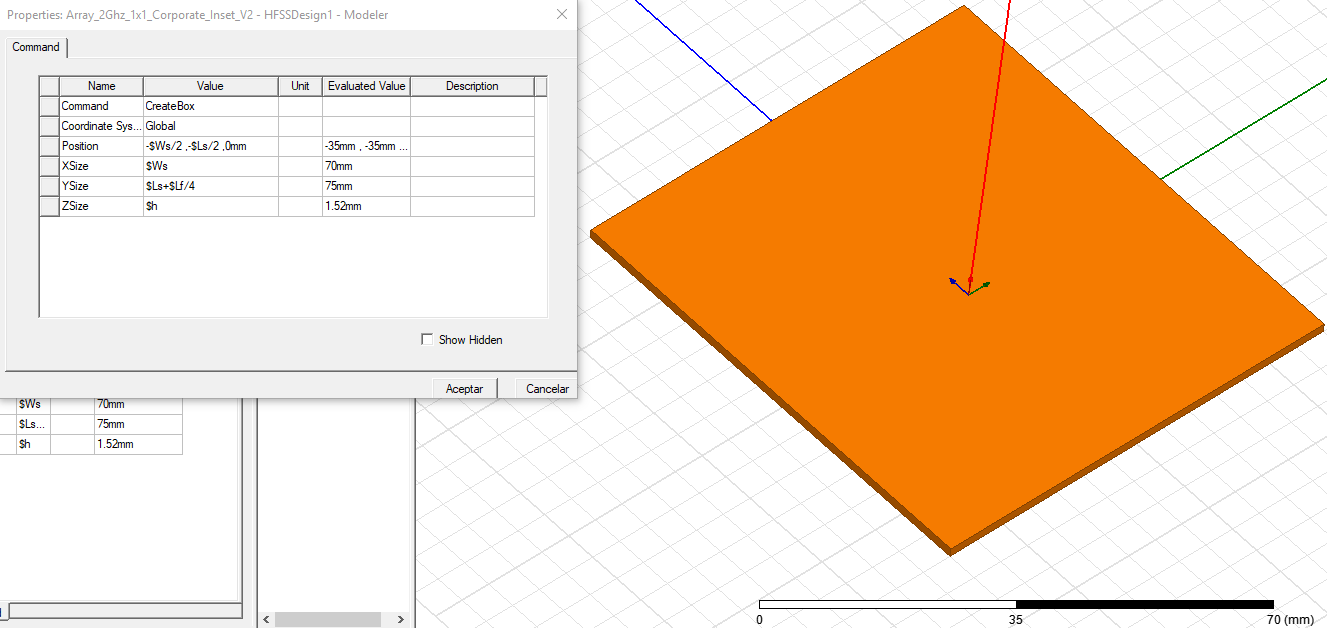
\includegraphics[width=13cm]{archivos/desarrollo/1}
        \caption{Creación del substrato}
        \label{fig:substrato}
\end{figure}
\par El plano de masa se creará mediante un plano simple. Para ello se usará la herramienta \textit{Draw Rectangle}, de igual manera que con el substrato, se le asignarán las variables idénticas a las asignadas al substrato, puesto que ambos tendrán el mismo ancho y alto, y se configurará su posición para que este esté centrado y pegado al plano inferior del substrato (fig. \ref{fig:masa}).
\\
\begin{figure}[h]
    \centering
        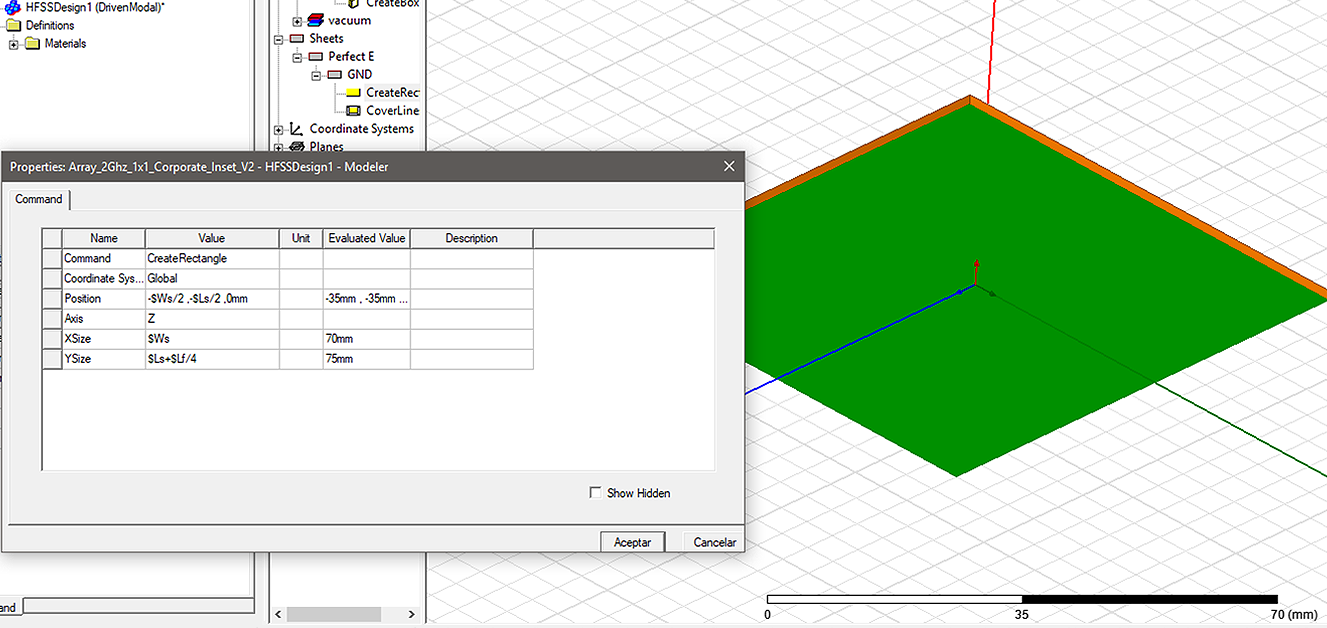
\includegraphics[width=13cm]{archivos/desarrollo/2}
        \caption{Creación del plano de masa}
        \label{fig:masa}
\end{figure}
\par A continuación, se volverá al plano superior del substrato, y volviendo a usar la herramienta \textit{Draw Rectangle} se creará un rectángulo con las medidas de W y L como ancho y alto respectivamente. Este rectángulo será nuestro parche (fig. \ref{fig:parche}). Cabe destacar como, todo lo relacionado con el parche, y el resto de circuitos de alimentación estarán situados sobre el substrato, es decir, a 1.52 mm sobre el origen de coordenadas del diseño del HFSS. Se volverá a repetir el proceso para el feed de alimentación, que unirá en uno de los lados que definen la anchura del parche al lado paralelo más próximo que define el ancho del substrato (fig. \ref{fig:feed}).
\\ 
\begin{figure}[h]
    \centering
        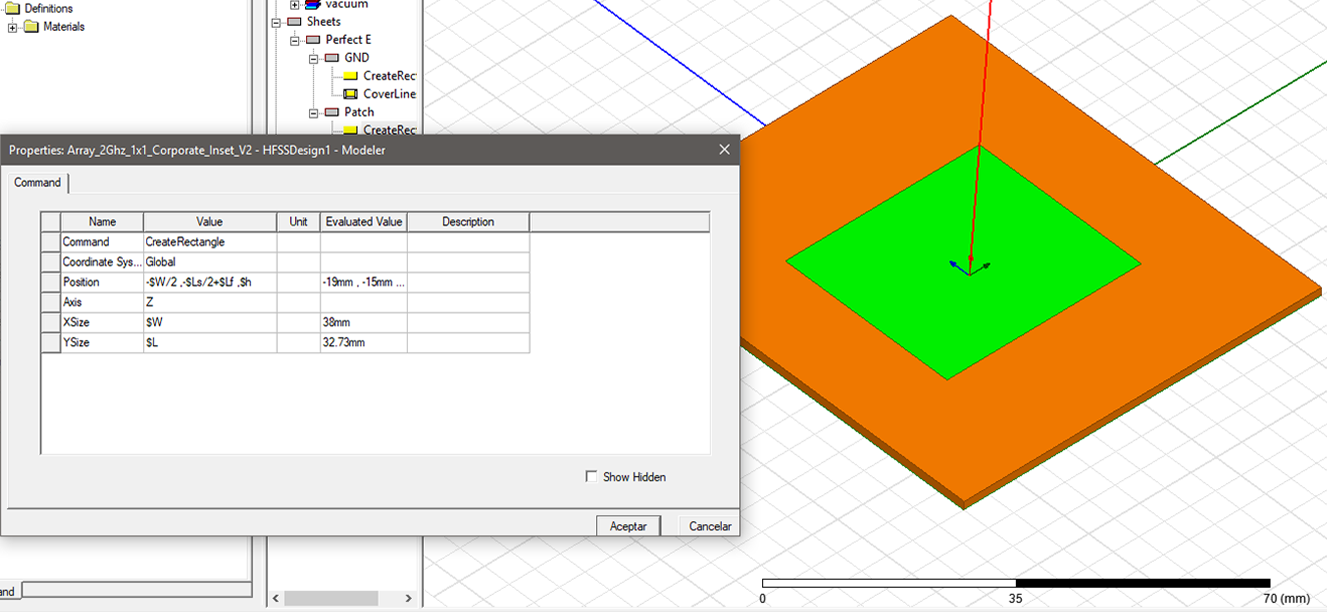
\includegraphics[width=13cm]{archivos/desarrollo/3}
        \caption{Creación del parche}
        \label{fig:parche}
\end{figure}
\begin{figure}[h]
    \centering
        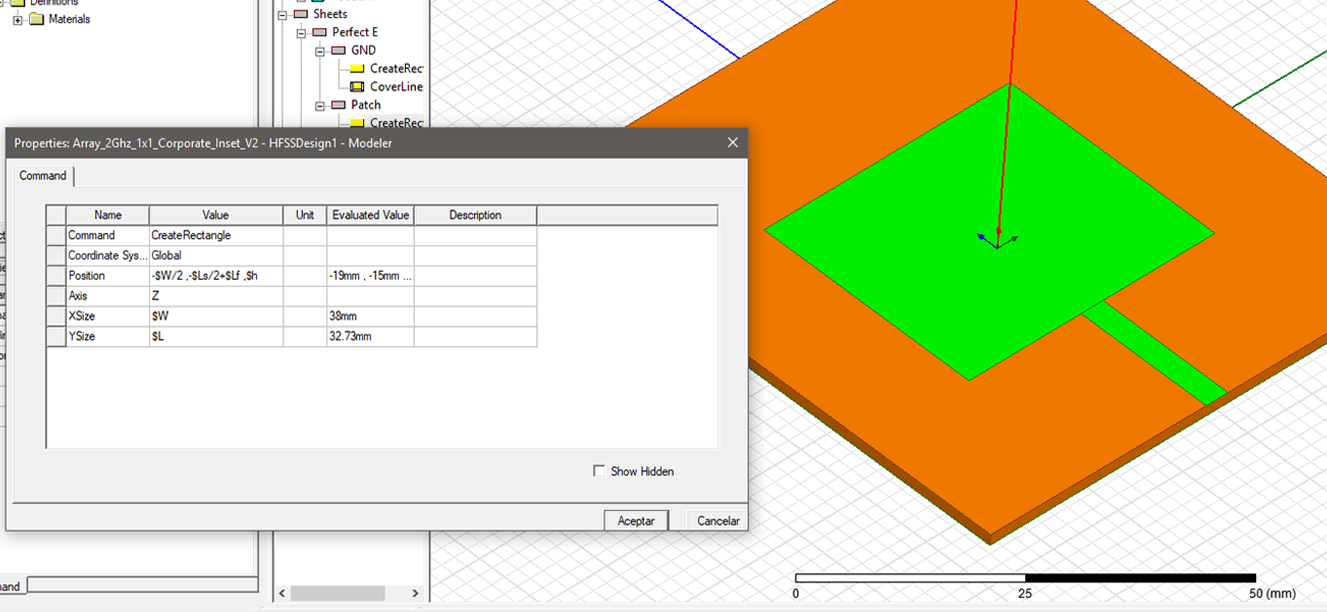
\includegraphics[width=13cm]{archivos/desarrollo/4}
        \caption{Creación del feed principal}
        \label{fig:feed}
\end{figure}
\par Seleccionando ahora los planos correspondientes a el \textit{feed} y el parche se procederá a pulsar el botón \textit{Unite}, que se encargará de unirlos como si fuera un solo material. Con este nuevo sólido que se habrá creado y seleccionando simultáneamente el rectángulo creado para el plano de masa se accederá a sus opciones y se pulsará sobre la opción \textit{Assign Boundary}>\textit{Perfect E}. De esta forma le daremos el comportamiento de conductor perfecto al conjunto de \textit{feed} y parche y al plano de masa (fig. \ref{fig:perfecte}). 
\\
\begin{figure}[h]
    \centering
        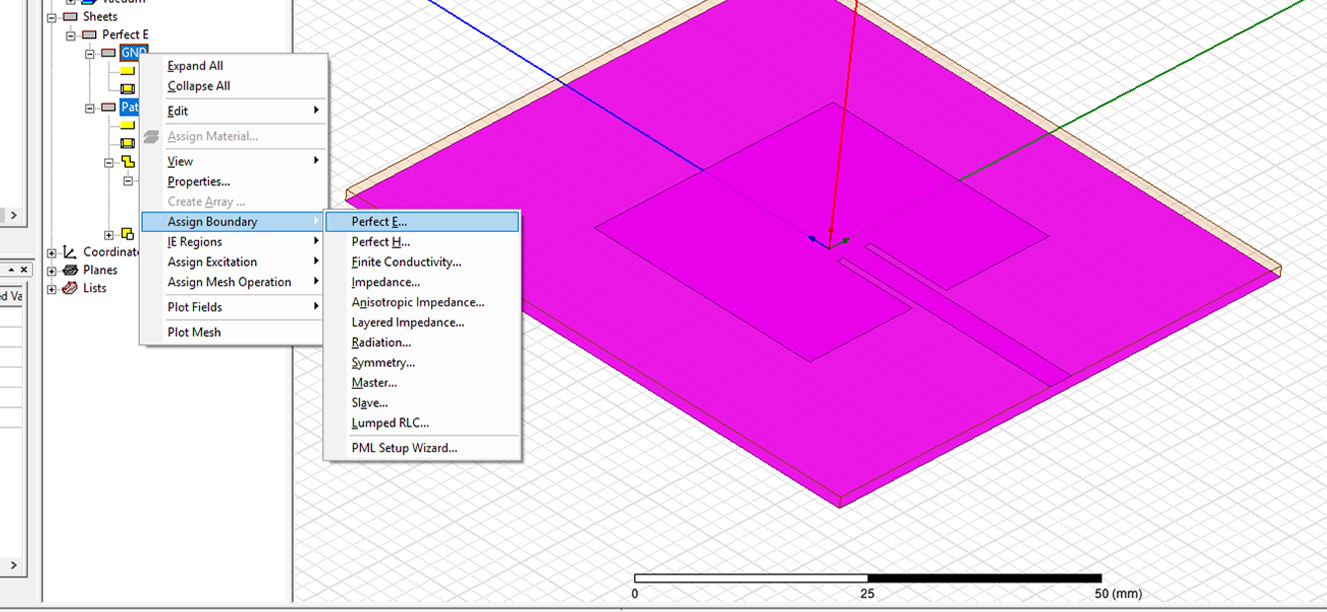
\includegraphics[width=13cm]{archivos/desarrollo/5}
        \caption{Asignación de material conductor al parche y al plano de masa}
        \label{fig:perfecte}
\end{figure}
\par Para excitar el sistema crearemos el \textit{Wave port}. Para ello se cambiará el plano de diseño de XY a ZX, para poder crear planos perpendiculares a los ya existentes en la antena. El \textit{Wave port} consistirá en un rectángulo que repose centrado sobre el extremo del substrato donde se puede acceder al \textit{feed}. Este debe tener unas dimensiones para cubrir el \textit{feed} por completo, así como tocar el plano de masa (fig. \ref{fig:waveport}). De la misma manera que se usó para asignar la propiedad de conductor al parche, se seleccionará sobre el plano creado para el \textit{Wave port} y en sus opciones aplicaremos: \textit{Assign Excitation}>\textit{WavePort}. 
\\

\begin{figure}[h]
    \centering
        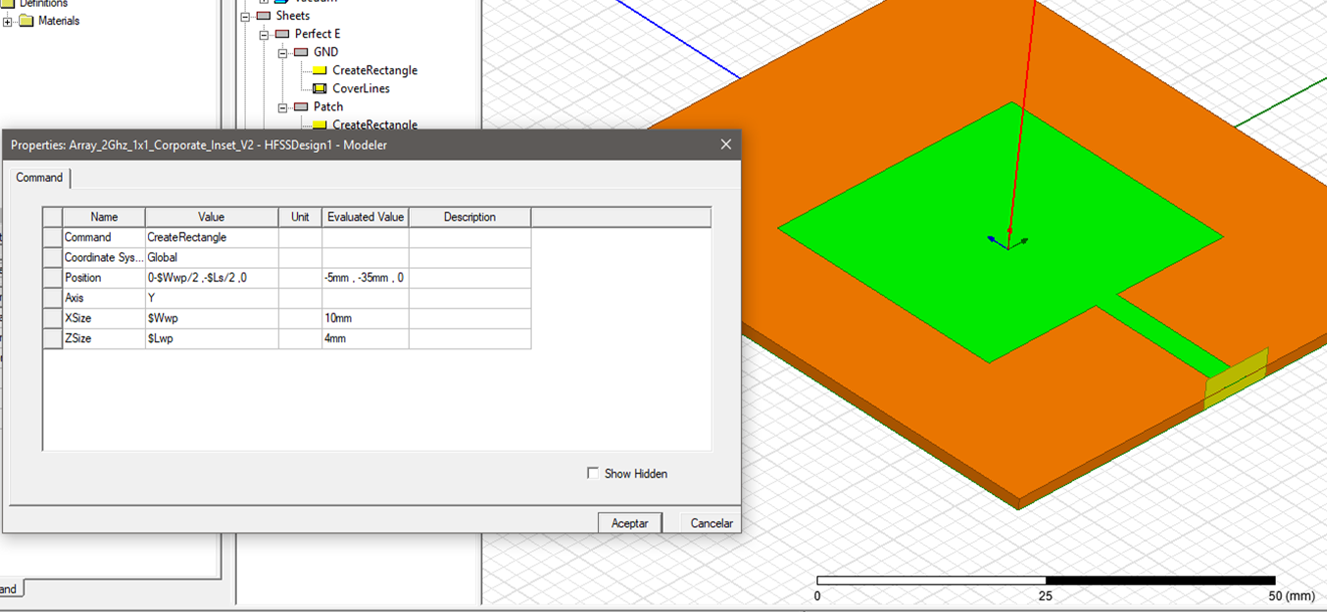
\includegraphics[width=13cm]{archivos/desarrollo/6}
        \caption{Creación del Wave-Port}
        \label{fig:waveport}
\end{figure}

\par Los dos ranuras o \textit{insets} que adaptarán el \textit{feed} y la antena, se crearán como rectángulos sobre el substrato y pegados al \textit{feed} dentro del parche (fig. \ref{fig:inseta}). Después, seleccionando el parche y ambos rectángulos se procederá, mediante el botón \textit{substract} a eliminar la superficie ocupara por los rectángulos, del plano del parche (fig. \ref{fig:insetb}). De esta forma se obtendrán las dos ranuras necesarias para conseguir la adaptación.
\\
\begin{figure}[H]
     \centering
     \begin{subfigure}[b]{0.45\textwidth}
         \centering
         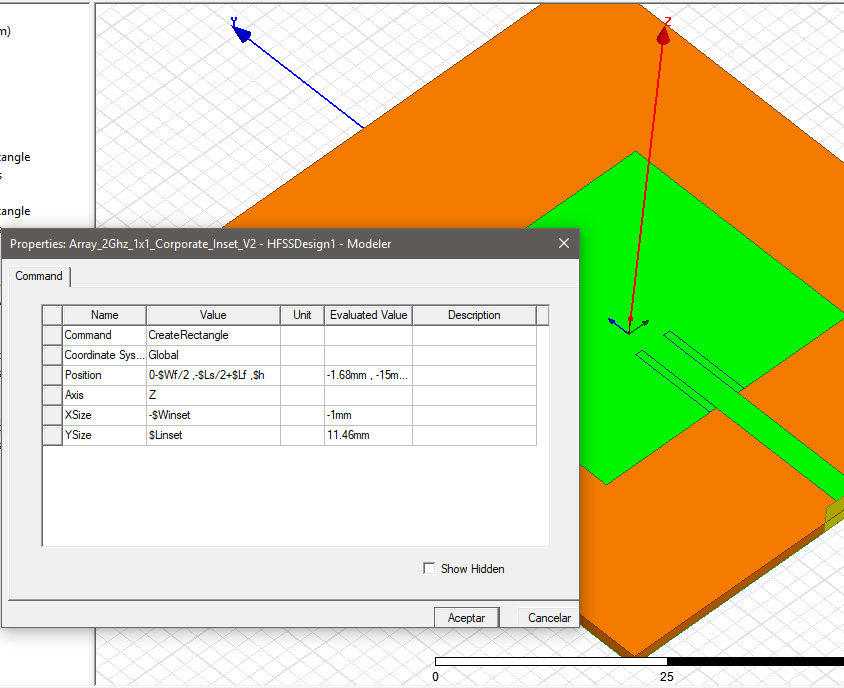
\includegraphics[width=\textwidth]{archivos/desarrollo/7a}
         \caption{Creación del \textit{inset} izquierdo}
         \label{fig:inseta}
     \end{subfigure}
     \hfill
     \begin{subfigure}[b]{0.45\textwidth}
         \centering
         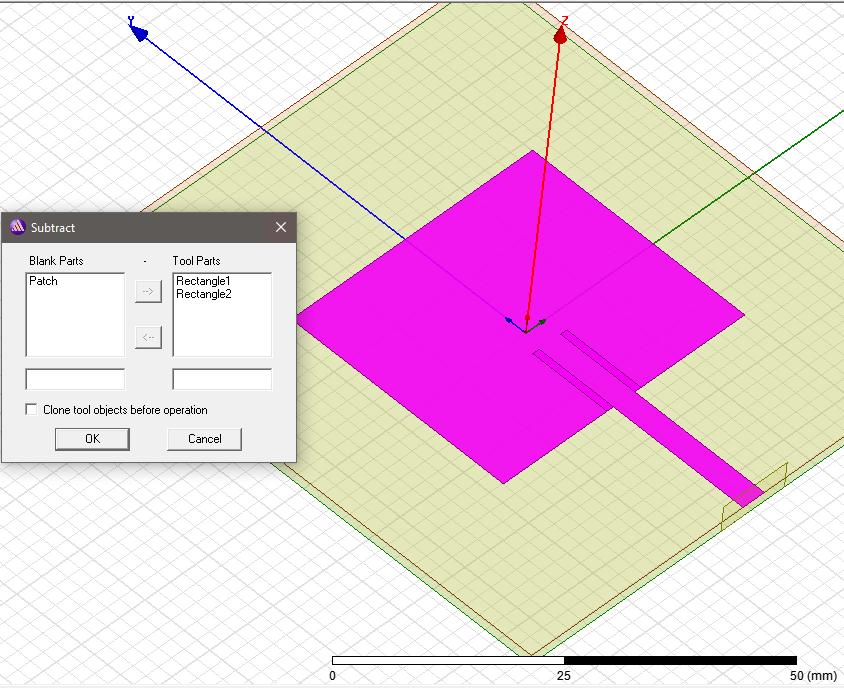
\includegraphics[width=\textwidth]{archivos/desarrollo/7b}
         \caption{Resta de la superficie de los \textit{insets}}
         \label{fig:insetb}
     \end{subfigure}
     \hfill
        \caption{Proceso de creación de los \textit{insets}}
        \label{fig:insets}
\end{figure}

\begin{figure}[h]
    \centering
        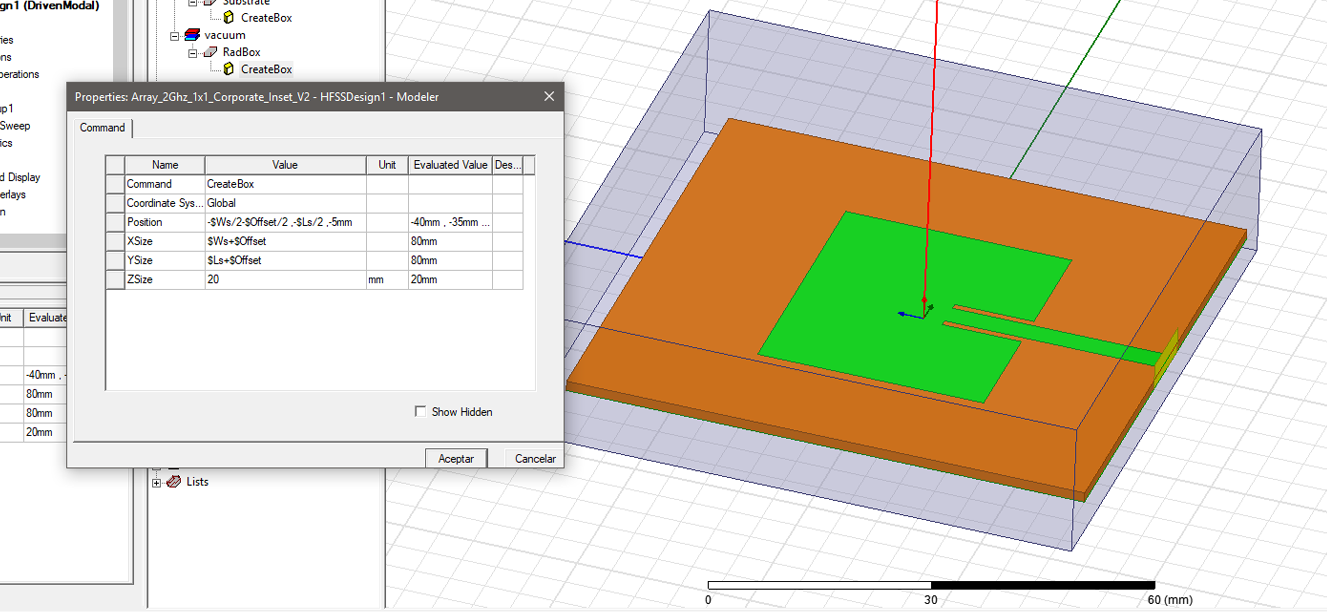
\includegraphics[width=13cm]{archivos/desarrollo/8}
        \caption{Creación del la caja de radiación}
        \label{fig:caja}
\end{figure}

\begin{figure}[H]
     \centering
     \begin{subfigure}[b]{0.48\textwidth}
         \centering
         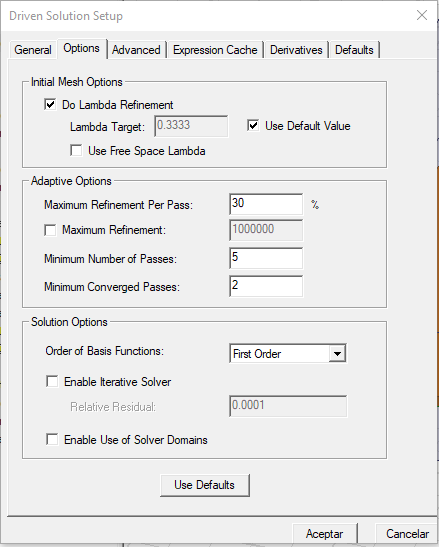
\includegraphics[width=\textwidth]{archivos/desarrollo/9a}
         \caption{Opciones de la configuración general}
         \label{fig:configa}
     \end{subfigure}
     \hfill
     \begin{subfigure}[b]{0.48\textwidth}
         \centering
         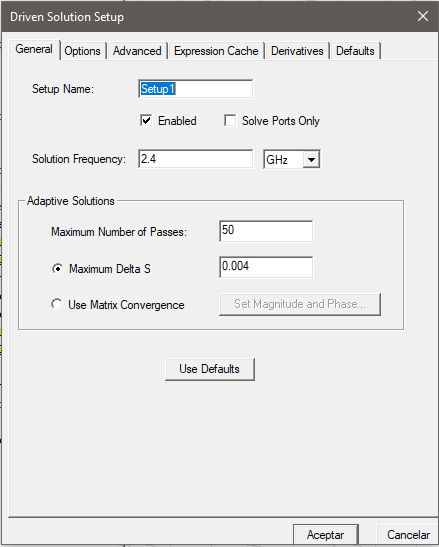
\includegraphics[width=\textwidth]{archivos/desarrollo/9b}
         \caption{Opciones de las iteraciones}
         \label{fig:configb}
     \end{subfigure}
     \hfill
     \\
     \begin{subfigure}[b]{0.48\textwidth}
         \centering
         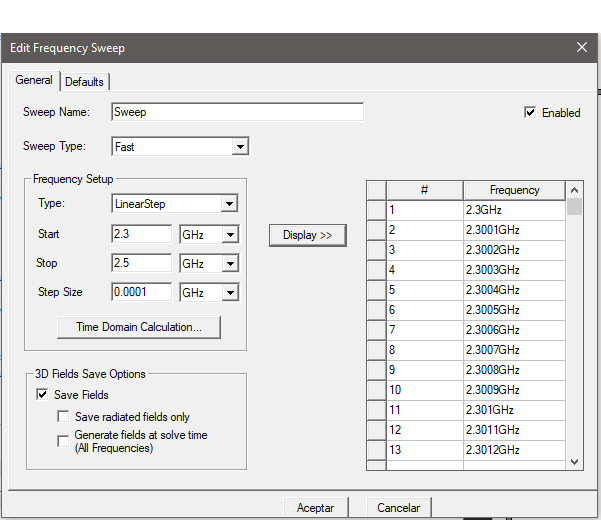
\includegraphics[width=\textwidth]{archivos/desarrollo/9c}
         \caption{Creación del barrido en frecuencia}
         \label{fig:configc}
     \end{subfigure}
     \hfill
        \caption{Configuración del simulador}
        \label{fig:config}
\end{figure}
\par El último elemento de diseño que se implementará será la caja de radiación. Esta se creará mediante la herramienta \textit{Draw box}, como se hizo con el substrato, y sus dimensiones deben ser capaces de cubrir el sistema entero que antena que se ha diseñado. Además, es importante el lado de la caja de radiación en el que se encuentra el \textit{Wave port} esté en el superpuesto en el plano de este (fig. \ref{fig:caja}). Además, de la misma forma que se hizo con elementos anteriores, se le asignará a este caja la propiedad de caja de radiación mediante: \textit{Assign Boundary}>\textit{Radiation} y como material: vacío.
\\
\par Llega el momento de configurar la simulación. Todas las opciones respecto a las iteraciones que va a realizar HFSS sobre el diseño se encuentran en la opción \textit{Analysis}, en sus opciones pulsaremos sobre \textit{Add Solution Setup}. En ella se introducirán los parámetros que se consideren necesarios para la correcta simulación del sistema. La frecuencia se ha establecido a 2.4 GHz \todo{fijarse en todos los GHz, todos lo que termine en "os", WavePorts}, el número máximo de pasadas como 50, y la máxima variación sobre el parámetro S de 0.004 (fig. \ref{fig:configa}). Si se entra a la pestaña \textit{options} se podrá también configurar parámetros como el número mínimo de pasadas, o el número mínimo de iteraciones consecutivas convergentes (fig. \ref{fig:configb}).
\\
\par Una vez creada la configuración del simulador, se añadirá el barrido en frecuencia sobre esta. Para ello, se añadirá un \textit{Frequency Sweep} mediante las opciones disponibles al pulsar sobre la configuración que hemos creado. En nuestro caso se configurará el barrido para crear un vector de frecuencias desde 2.3 GHz hasta 2.5 GHz cada 0.0001 GHz, creando un total de 1001 puntos de frecuencia para así obtener una mayor resolución en las gráficas que se deseen mostrar. El tipo de sweep se seleccionará como \textit{fast}, lo que ayudará a la máquina a agilizar el proceso de cálculo y es importante marcar la opción \textit{Save fields} para poder, más tarde, mostrar los datos relacionados con el campo lejano.
\\
\par Ya estaría listo el diseño y la configuración del solucionador para lanzar la simulación del sistema. Para ello se pulsará primero sobre el botón \textit{Validate} para confirmar que todo está correctamente configurado y no hay errores en el diseño que impidan que HFSS no pueda iniciar la simulación. Tras comprobar que no existen errores, mediante el botón \textit{Analyze all} se podrá iniciar la simulación. Durante la simulación HFSS irá realizando iteraciones en las que los tetraedros se irán adaptando a nuestro parche (fig. \ref{fig:tetra}). En cada iteración el número de tetraedros irá creciendo exponencialmente (fig. \ref{fig:conver}), con lo que es posible que en las últimas iteraciones, el simulador tarde más en realizar una pasada completa. Si se pulsa sobre la opción \textit{Convergence} dentro de las opciones del configurador de la simulación, se podrá obvservar de forma gráfica o anaítica el número de pasadas que ha realizado el simulador (fig. \ref{fig:convera}) así como otros datos sobre la convergencia de la simulación.
\\

\begin{figure}[H]
     \centering
     \begin{subfigure}[b]{0.47\textwidth}
         \centering
         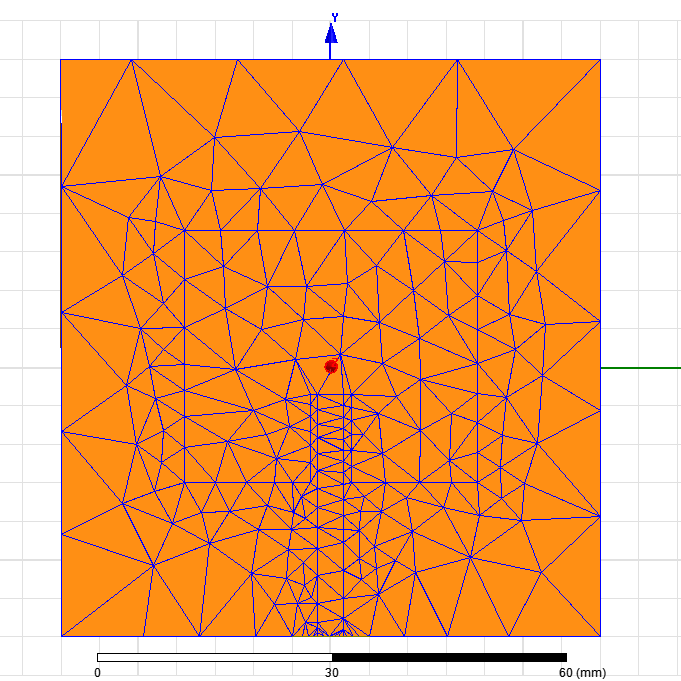
\includegraphics[width=\textwidth]{archivos/desarrollo/10a}
         \caption{Distribución de tetraedros en la iteración nº5}
         \label{fig:tetraa}
     \end{subfigure}
     \hfill
     \begin{subfigure}[b]{0.47\textwidth}
         \centering
         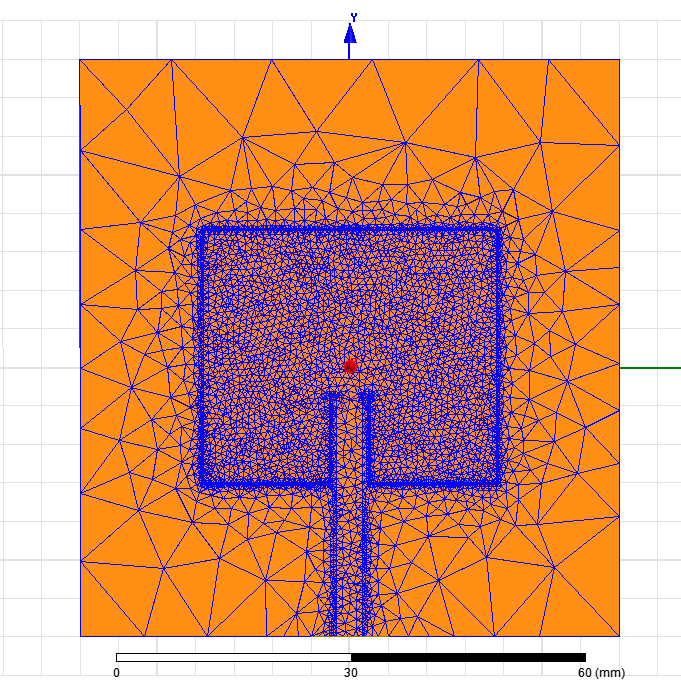
\includegraphics[width=\textwidth]{archivos/desarrollo/10b}
         \caption{Distribución de tetraedros en la iteración nº27}
         \label{fig:tetrab}
     \end{subfigure}
     \hfill
        \caption{Tetraedros creados por HFSS para calcular el comporamiento del sistema}
        \label{fig:tetra}
\end{figure}

\begin{figure}[H]
     \centering
     \begin{subfigure}[b]{0.47\textwidth}
         \centering
         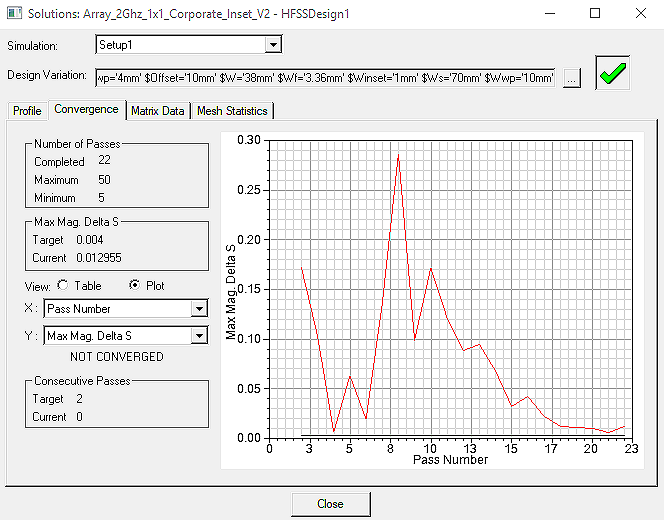
\includegraphics[width=\textwidth]{archivos/desarrollo/11a}
         \caption{Histórico de \textit{Delta S}}
         \label{fig:convera}
     \end{subfigure}
     \hfill
     \begin{subfigure}[b]{0.47\textwidth}
         \centering
         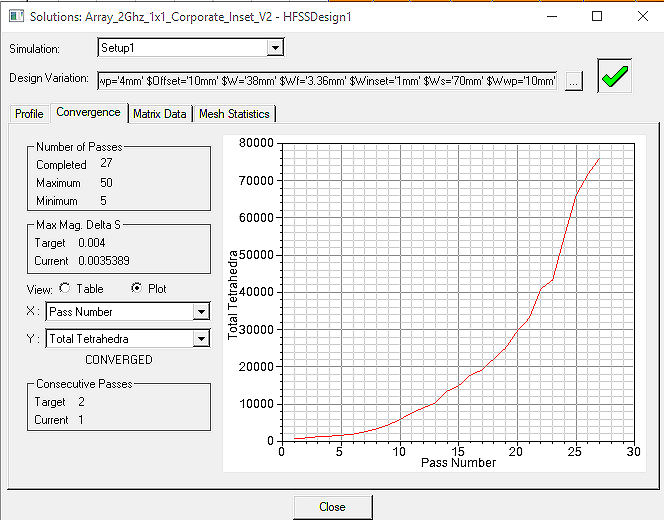
\includegraphics[width=\textwidth]{archivos/desarrollo/11b}
         \caption{Numero de tetraedros en la iteración nº27}
         \label{fig:converb}
     \end{subfigure}
     \hfill
        \caption{Datos sobre la simulación actual}
        \label{fig:conver}
\end{figure}

\par Una vez que la simulación ha convergido, HFSS empezará con otra serie de cálculos. Principalmente cálculos matriciales relacionados con los datos obtenidos de la simulación. Tras su finalización, se podrá proceder a analizar los resultados. Las gráficas de los resultados se obtienen mediante la pestalla \textit{Results}. Allí, al pulsar sobre sus opciones, se podrán acceder a diferentes tipos de representaciones según la naturaleza de esta: Reportes sobre soluciones modales, reportes sobre el campo lejano, etc. En primer lugar se analizará la curva de pérdida de retorno, o parámetro S, que se puede encontrar dentro de: \textit{Create Modal Solution Data Report}>\textit{Rectángular Plot}. Se abrirá una ventana donde se podrá seleccionar qué parámetro se quiere graficar, en nuestro caso \textit{S Parameter} en dB. En la misma ventana y dentro de la pesataña \textit{Families} se podrá seleccionar qué variación de nuestro diseño se quiere graficar, en el caso de que se hayan realizado más de una simulación con cambios en el diseño entre ellas. Finalmente, se pulsará sobre \textit{New Report} para ver el resultado.
\\
\par Como se mencionó al final de la sección \ref{351} Los resultados obtenidos mediante las dimensiones proporcionadas por las ecuaciones que se implementaron en MATLAB han de ser refinados, ya que estos no harán que nuestra antena funcione exactamente de la manera en la que se desea. Es necesario un trabajo previo al resultado final, basado en iteraciones propias realizadas por el ingeniero, en las que se modifiquen ciertas dimensiones de la antena para encontrar la solución que este busque. En el caso de esta antena, los resultados obtenidos tras el trabajo previo, en el que se han reducido 2 mm el ancho de la antena, se pueden ver a continuación. Cabe mencionar que, a lo largo del análisis de los resultados de nuestros diseños, se omitirá este proceso de refinado del diseño, y se mostrarán directamente las dimensiones con las que se ha encontrado que la antena trabaja según las especificaciones deseadas.
\\
\begin{itemize}
\item \textbf{Gráfica de pérdidas de retorno o parámetro S: }Se puede observar un buen comportamiento de la antena, con unas pérdidas de retorno en la frecuencia de trabajo de 2.4 GHz de -39.53 dBs, suficiente para el correcto funcionamiento de la antena a esta frecuencia, así como un ancho de banda a -10 dBs de de 36.5 MHz, lo que equivale a un 1.56\% sobre la frecuencia de trabajo.
	\begin{figure}[H]
    \centering
        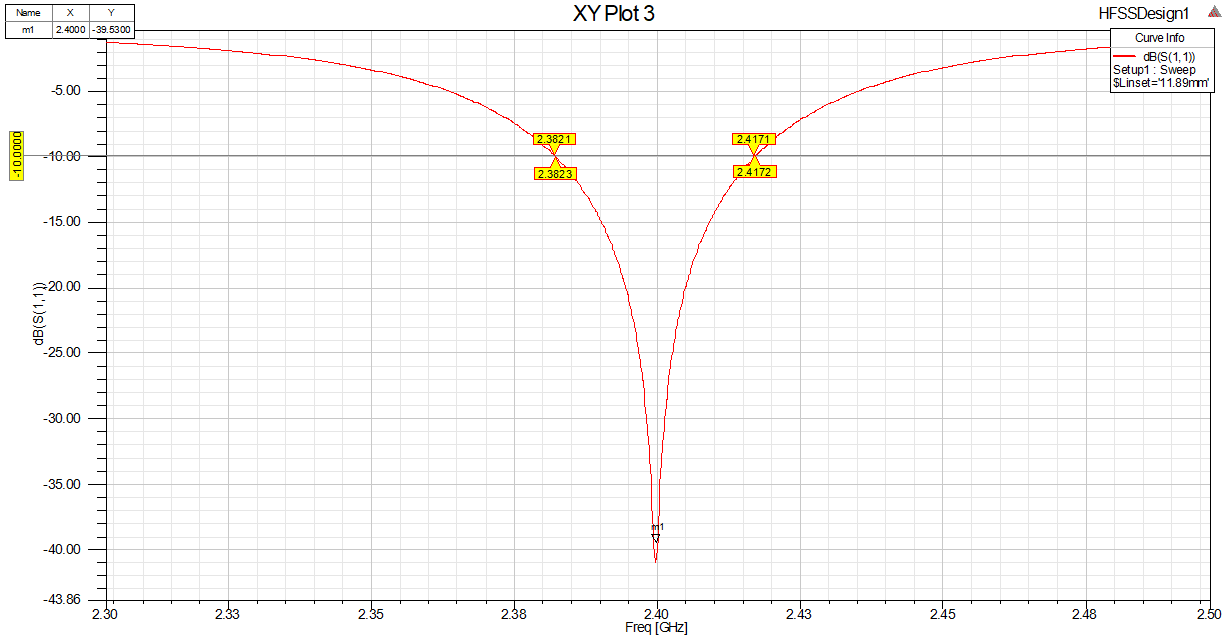
\includegraphics[width=14cm]{archivos/desarrollo/12a}
        \caption{Pérdidas de retorno}
        \label{fig:s}
	\end{figure}
	
\item \textbf{Gráfica del componente real de la impedancia: }En esta gráfica el objetivo principal es encontrar un valor de 50 $\Omega$ para la frecuencia de trabajo de 2.4 GHz. Este valor influencia directamente a la curva del parámetro S. Como se puede observar, el valor obtenido de 51 $\Omega$ lo que significa que la adaptación final entre el sistema de alimentación y la antena ha sido correcta.
	\begin{figure}[H]
    \centering
        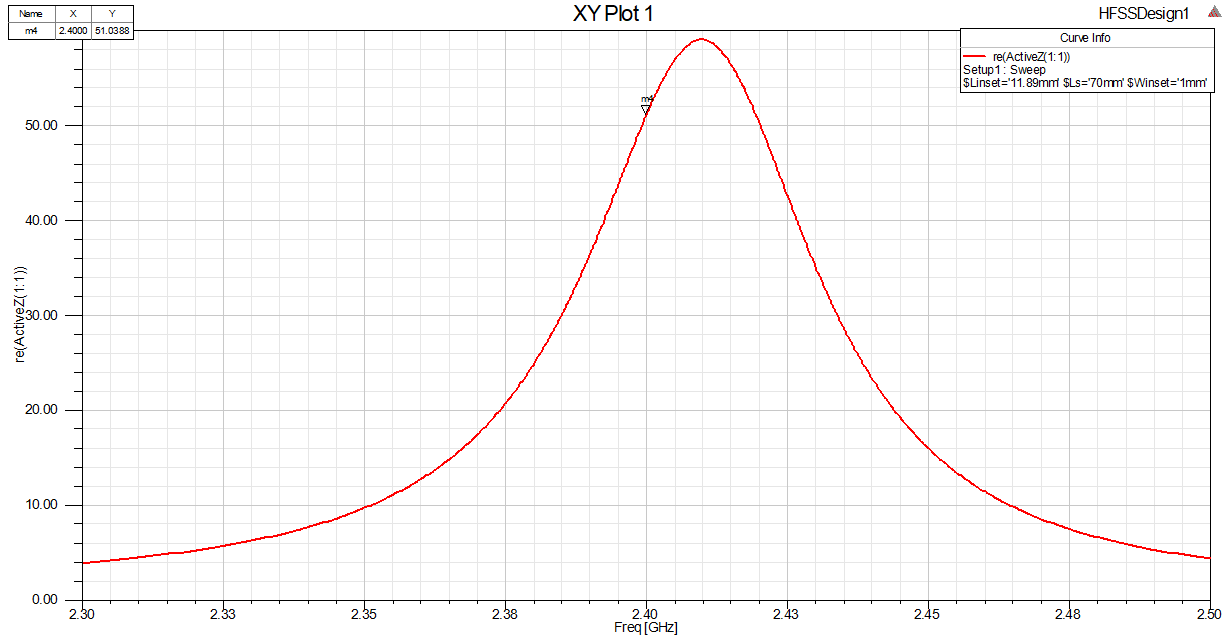
\includegraphics[width=14cm]{archivos/desarrollo/12b}
        \caption{Componente óhmica de la impedancia}
        \label{fig:realimpe}
	\end{figure}
	
\item \textbf{Gráfica del componente imaginaria de la impedancia: }En este caso, el cometido es encontrar un nulo de la curva de la componente reactiva de la impedancia para la frecuencia de trabajo. El valor obtenido para este diseño es de 0.23 $\Omega$, lo que puede considerarse como un buen resultado en el diseño.
	\begin{figure}[H]
    \centering
        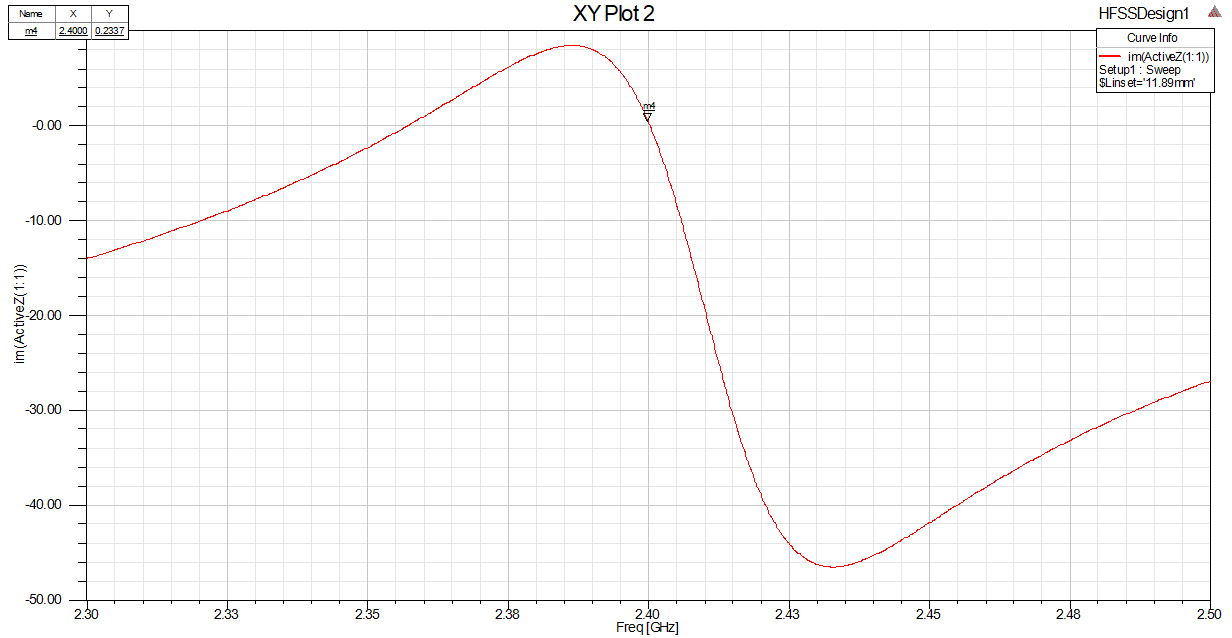
\includegraphics[width=14cm]{archivos/desarrollo/12c}
        \caption{Componente reactiva de la impedancia}
        \label{fig:imaimpe}
	\end{figure}

\item \textbf{Patrón de radiación en el plano E: }El patrón de radiación para el plano E, es aquel en el que se cumple que $\phi $ = 0º. En concreto el patrón de radiación que se mostrará a lo largo del proyecto es el correspondiente al de la directividad de la antena, medido en decibelios y en forma polar. Como se puede comprobar, el resultado obtenido es un patrón de radiación omnidireccional a lo largo del plano superior de la antena y un pequeño lóbulo trasero en el plano inferior. La directividad máxima de la antena, donde $\Theta$ = 0/360º, es de 5.36 dB. 
	\begin{figure}[H]
    \centering
        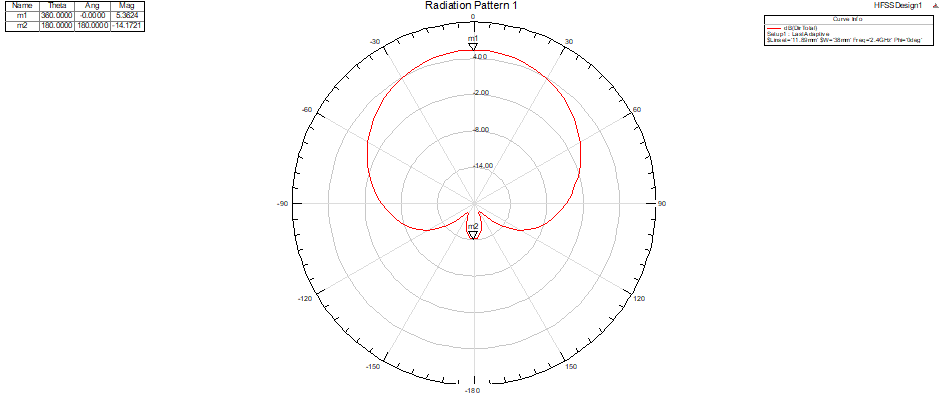
\includegraphics[width=14cm]{archivos/desarrollo/12d}
        \caption{Patrón de radiación del plano E}
        \label{fig:radE}
	\end{figure}

\item \textbf{Patrón de radiación en el plano H: }Repetiremos el proceso seguido para obtener el patrón de radiación en el plano E, pero con la principal diferencia de que el plano H es perpendicular a este, es decir, $\phi $ = 90º. Al tratarse de un parche único, no influenciado por otras antenas, el patrón de radiación en este plano es muy parecido al obtenido en la componente eléctrica, con una pequeña variación en la parte derecha del plano superior, producido por efectos conductores en la línea de alimentación microstrip. La directividad máxima obtenida en este plano es de 5.36 dB.
	\begin{figure}[H]
    \centering
        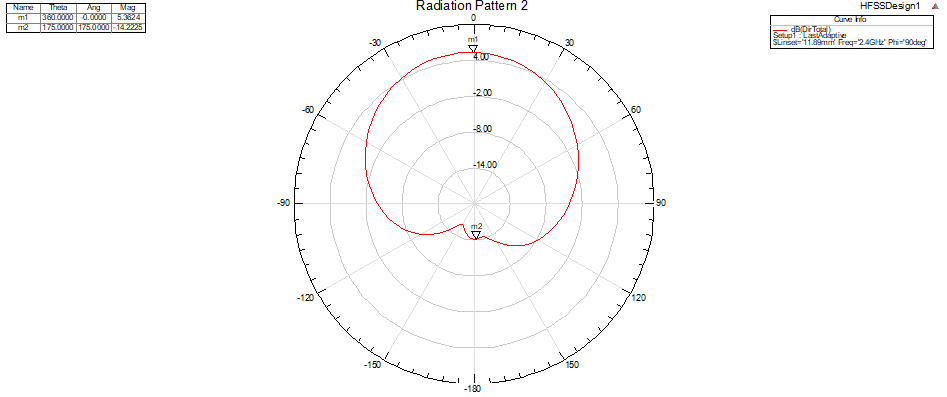
\includegraphics[width=14cm]{archivos/desarrollo/12e}
        \caption{Patrón de radiación del plano H}
        \label{fig:radH}
	\end{figure}

\item \textbf{Patrón de radiación tridimensional: }Aunque hemos mostrado los patrones de directividad para los ángulos $\phi $ en 0º y 90º, HFSS los calcula para la circunferencia completa. Se puede recrear el patrón de radiación en trews dimensiones si representamos juntos los patrones de dirección para todos los ángulos de $\phi$ y $\Theta$. HFSS ofrece una manera sencilla de hacerlo. Como se puede observar en los resultados, hemos obtenido una antena completamente omnidireccional para el plano superior del parche y una directividad casi nula en el plano inferior, lo que podríamos asimilar a un monopolo. La directividad obtenida siempre coincidirá con uno de los máximos, del campo E o H, en este caso 5.36 dB.
	\begin{figure}[H]
    \centering
        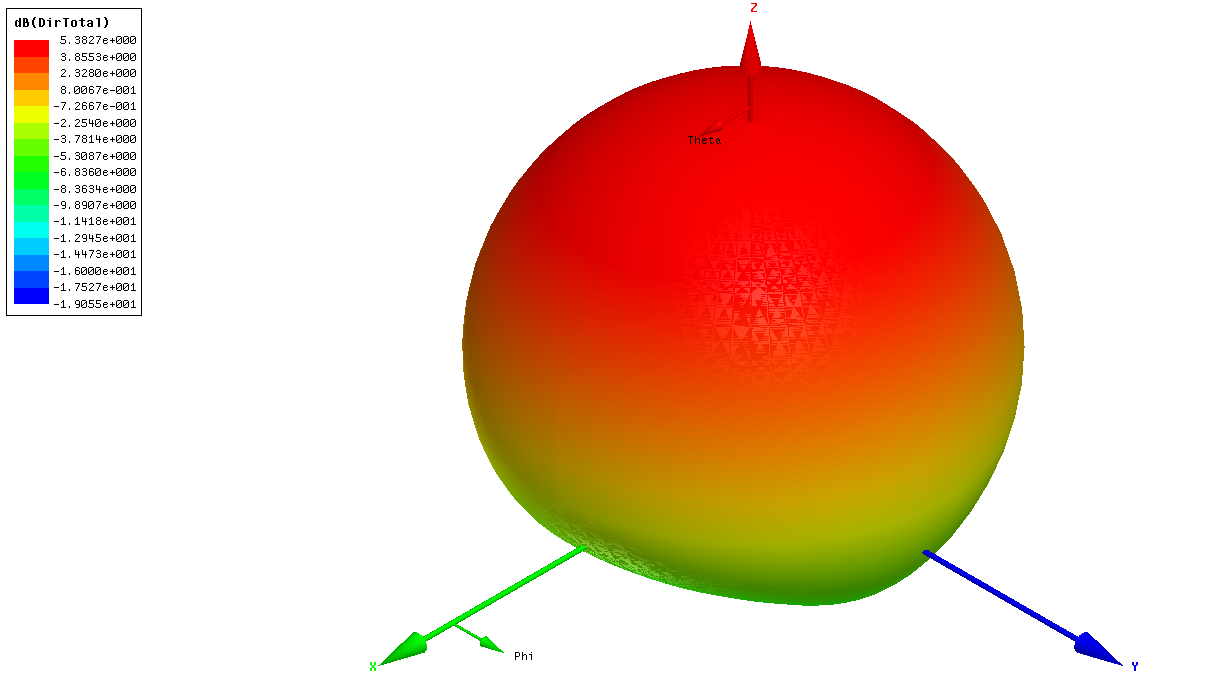
\includegraphics[width=11cm]{archivos/desarrollo/12f}
        \caption{Patrón de radiación 3D}
        \label{fig:rad3d}
	\end{figure}
	
\item \textbf{Distribución eléctrica sobre la antena: }Otro tipo de análisis que podemos realizar sobre la antena consiste en la muestra directa sobre la antena de ciertos parámetros como el campo eléctrico, los vectores de los campos eléctricos y magnéticos, etc. En este caso, se muestra la distribución del campo eléctrico sobre la antena. En el se pueden observar donde se sitúan los principales valles y nodos sobre esta.
	\begin{figure}[H]
    \centering
        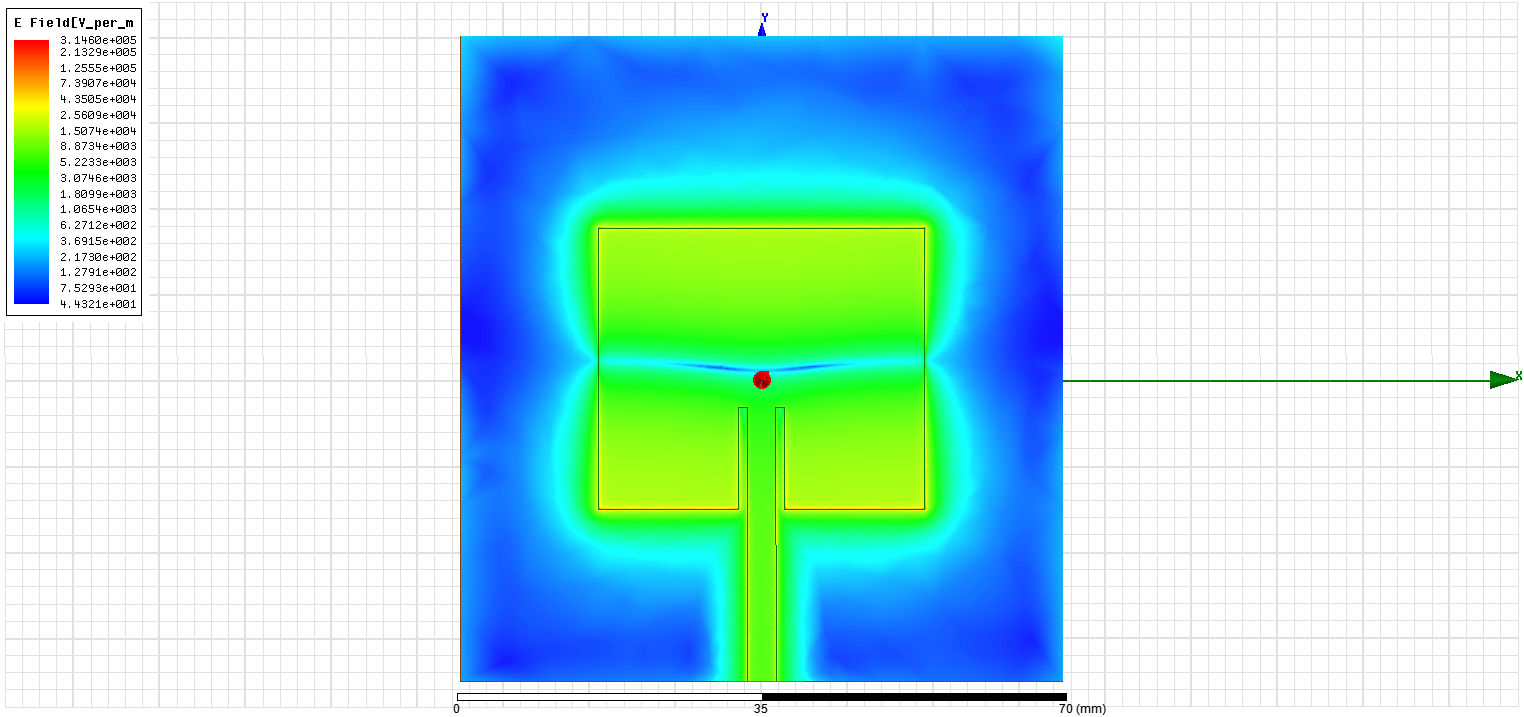
\includegraphics[width=12cm]{archivos/desarrollo/12g}
        \caption{Campos eléctricos en la superficie de la antena}
        \label{fig:Complexmage}
	\end{figure}

\end{itemize}

\subsection{Análisis de los diseños}
\par Ahora que se conoce cómo es el proceso de diseño de un parche microstrip en HFSS se procederá a implementar las distintas configuraciones anteriormente mencionadas. Durante esta sección serán comentados principalmente los aspectos sobre el diseño que conciernen a las antenas, y se dejará para el siguiente capítulo el análisis de los resultados obtenidos. Durante el análisis de los diseños repasaremos en diferentes secciones cada configuración de array para ambas frecuencias en la que han sido diseñadas, y finalmente se mencionará el caso del diseño a 27 Ghz. Es importante remarcar que \textbf{todas las acotaciones mostradas a lo largo de esta sección estarán en milímetros} y se han decidido omitir para mejorar la legibilidad de las imágenes.

\subsubsection{Parche simple} 
\par La antena microtrip simple de un único parche ha sido la antena estudiada en la sección anterior para el caso de 2.4 Ghz. Se trata de una antena muy simple, alimentada mediante una línea microstrip directa cuya impedancia está referenciada a 50 $\Omega$.
\\
\par En la tabla \ref{tab:simple1} y \ref{tab:simple2} se pueden observar las diferencias entre los resultados proporcionados por el script de MATLAB y los aplicados finalmente en el diseño de la antena para el caso del parche de 2.4 GHz.

\begin{table}[H]
  
   \label{tab:simple1}
   \small % text size of table content
   \centering % center the table
   \begin{tabular}{m{0.2\linewidth}m{0.25\linewidth}m{0.25\linewidth}} % alignment of each column data
   \toprule[\heavyrulewidth]\toprule[\heavyrulewidth]
   \textbf{Parámetro} & \textbf{Dimensión MATLAB} & \textbf{Dimensión final} \\ 
   \midrule
   \textbf{W} & 41.40 mm & 38 mm \\
   \textbf{L} & 32.73 mm & 32.73 mm\\
   \textbf{Linset} & 11.89 mm & 11.89 mm\\
   \textbf{Winset} & - & 0.5 mm\\
   \textbf{W50} & 3.36 mm & 3.36 mm\\
   \textbf{Ws/Ls} & - & 70 mm\\
   \bottomrule[\heavyrulewidth] 
   \end{tabular}
   \caption{Dimensiones de parche único microstrip a 2.4 GHz} 
\end{table}

\begin{table}[H]
  
   \label{tab:simple2}
   \small % text size of table content
   \centering % center the table
   \begin{tabular}{m{0.2\linewidth}m{0.25\linewidth}m{0.25\linewidth}} % alignment of each column data
   \toprule[\heavyrulewidth]\toprule[\heavyrulewidth]
   \textbf{Parámetro} & \textbf{Dimensión MATLAB} & \textbf{Dimensión final} \\ 
   \midrule
   \textbf{W} & 16.56 mm & 17.9 mm \\
   \textbf{L} & 12.64 mm & 12.64 mm\\
   \textbf{Linset} & 4.57 mm & 4.5 mm\\
   \textbf{Winset} & - & 0.5 mm\\
   \textbf{W50} & 3.34 mm & 3.42 mm\\
   \textbf{Ws/Ls} & - & 40 mm\\
   \bottomrule[\heavyrulewidth] 
   \end{tabular}
   \caption{Dimensiones de parche único microstrip a 6 GHz} 
\end{table}

\par Como se puede observar, las dimensiones finales obtenidas tras la optimización de estas para encontrar el mejor resultado de los parámetros de la antena, se asemejan mucho a los proporcionados por MATLAB. Solo en el caso de la antena a 6 GHz hemos tenido que modificar los valores de \textit{W50} y \textit{Linset}. Por lo general, y comos se podrá comprobar también en el resto de las antenas posteriores, el mayor cambio a realizar para adaptar la antena a los resultados deseados, reside en la anchura del parche \textit{W}, así como, en menor parte, en la longitud de la ranura de adaptación \textit{Linset}.


\begin{figure}[H]
    \centering
        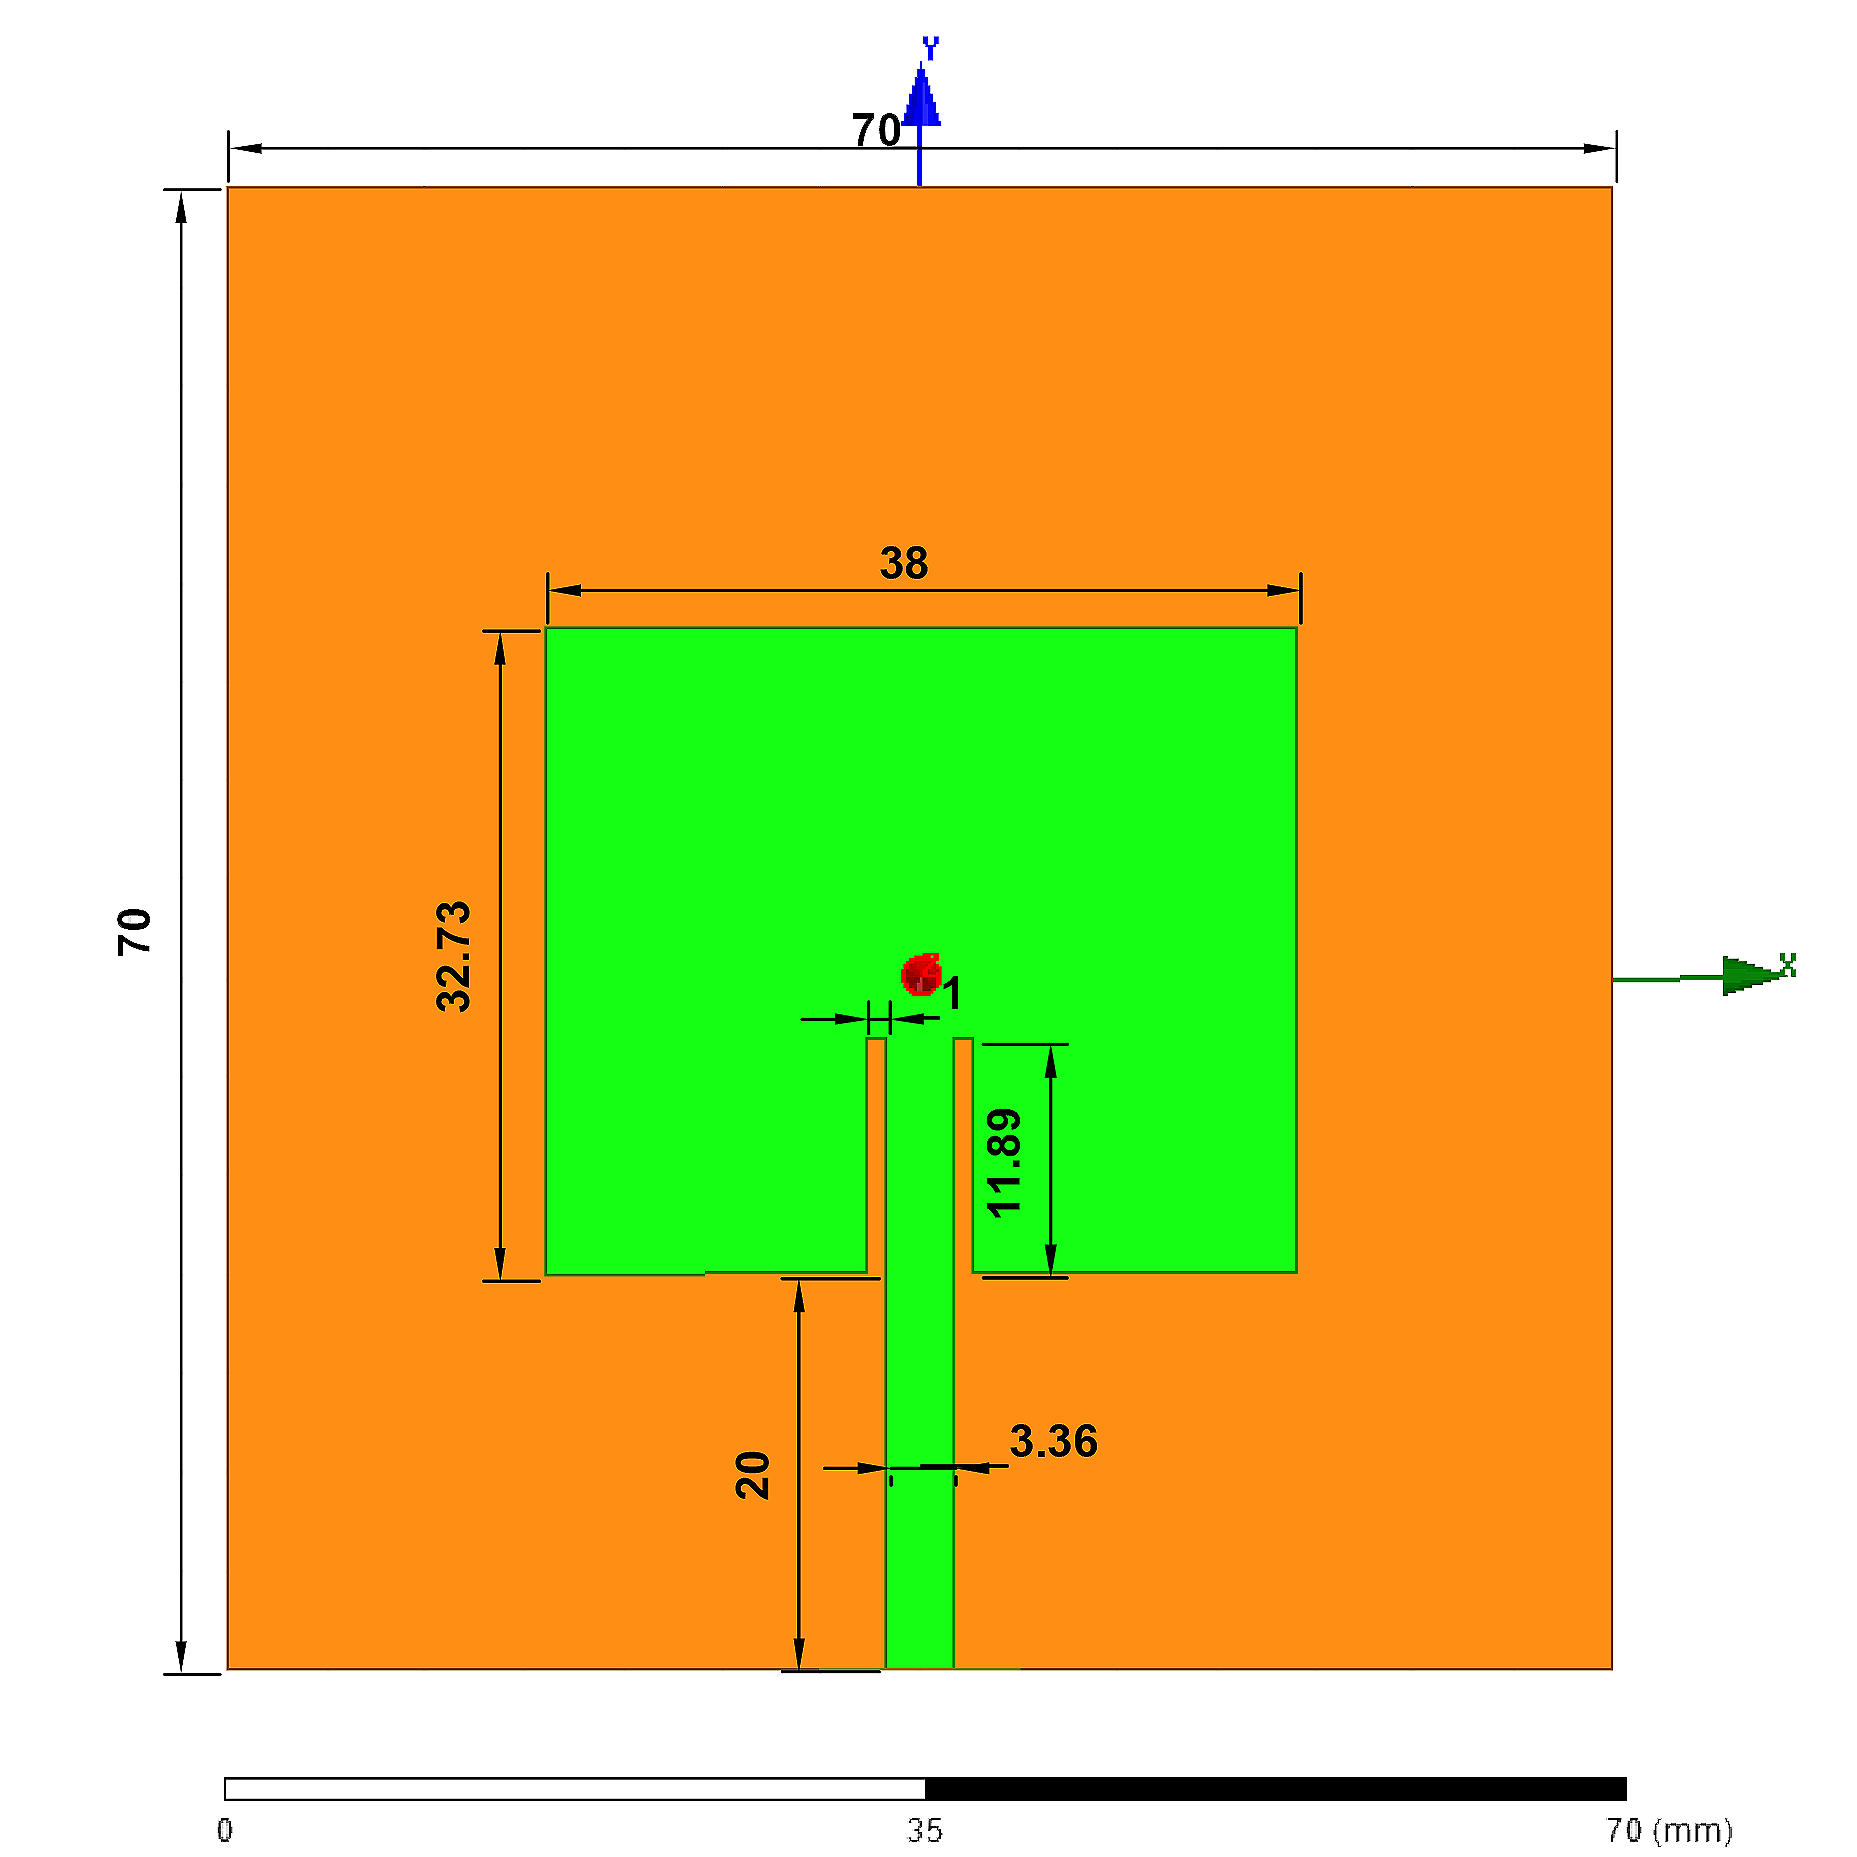
\includegraphics[width=12cm]{archivos/desarrollo/autocad/1}
        \caption{Parche simple a 2.4 Ghz}
         \label{fig:simple1}
\end{figure}

\begin{figure}[H]
    \centering
        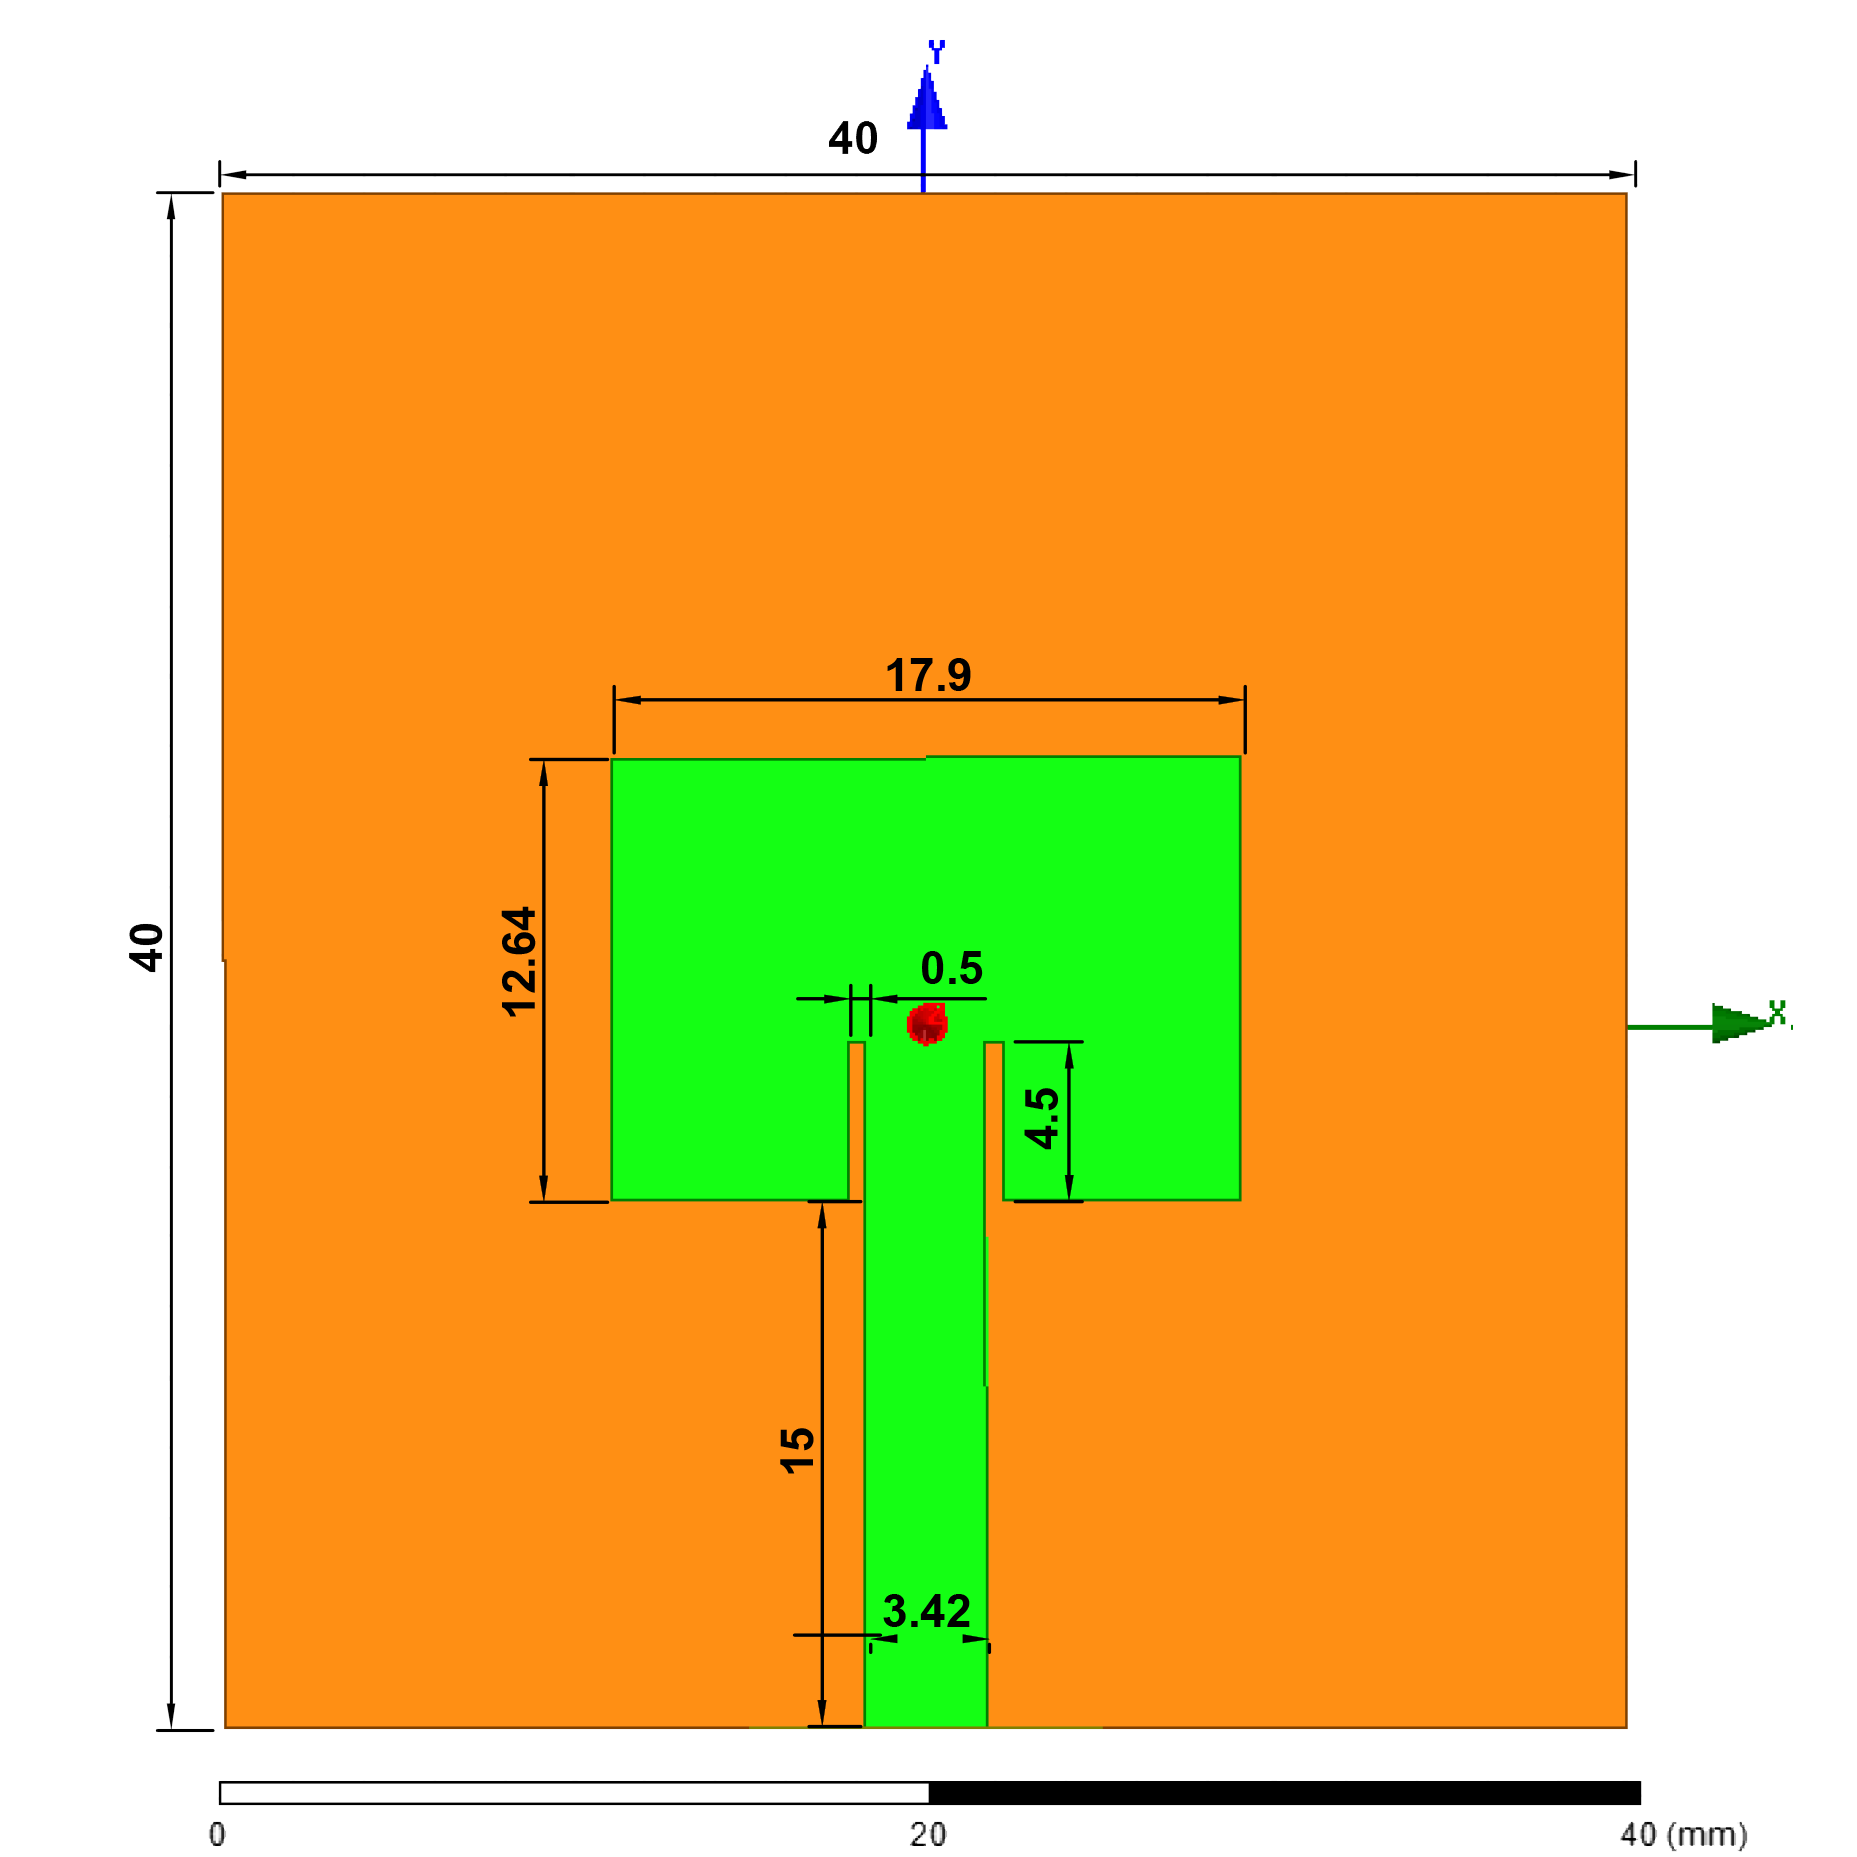
\includegraphics[width=12cm]{archivos/desarrollo/autocad/2}
        \caption{Parche simple a 6 Ghz}
         \label{fig:simple2}
\end{figure}




\subsubsection{Array 2x1 Paralelo} 
\par La primera configuración que hemos diseñado como producto de la unión de varios de parches simples se basa en la unión en paralelo de dos de estos parches. Como se mencionó con anterioridad, estos serán distanciados en una longitud de 0.7 veces la longitud de onda en el vacío $\lambda_{0}$. 
\\
\par Si se comparan los resultados obtenidos en MATLAB con respecto a los encontrados tras la optimización de las variables vemos que para el caso del array a 2.4 GHz los resultados obtenidos si que difieren de los proporcionados por MATLAB, aunque, como se verá más adelante, los resultados finales obtenidos con las nuevas dimensiones ofrecen a la antena las características deseadas. En el caso de la antena a 6 Ghz, los resultados si son casi idénticos a los proporcionados por MATLAB.

\begin{table}[h]
  
   \label{tab:array2x11}
   \small % text size of table content
   \centering % center the table
   \begin{tabular}{m{0.2\linewidth}m{0.25\linewidth}m{0.25\linewidth}} % alignment of each column data
   \toprule[\heavyrulewidth]\toprule[\heavyrulewidth]
   \textbf{Parámetro} & \textbf{Dimensión MATLAB} & \textbf{Dimensión final} \\ 
   \midrule
   \textbf{W} & 41.40 mm & 40.67 mm \\
   \textbf{L} & 32.73 mm & 32.29 mm\\
   \textbf{Linset} & 11.89 mm & 3.46 mm\\
   \textbf{Winset} & - & 0.52 mm\\
   \textbf{W50} & 3.36 mm & 2.84 mm\\
   \textbf{W100} & 0.85 mm & 2 mm\\
   \textbf{Ws/Ls} & - & 100/70 mm\\
   \bottomrule[\heavyrulewidth] 
   \end{tabular}
   \caption{Dimensiones de array 2x1 microstrip a 2.4 GHz} 
\end{table}

\begin{table}[h]
  
   \label{tab:array2x12}
   \small % text size of table content
   \centering % center the table
   \begin{tabular}{m{0.2\linewidth}m{0.25\linewidth}m{0.25\linewidth}} % alignment of each column data
   \toprule[\heavyrulewidth]\toprule[\heavyrulewidth]
   \textbf{Parámetro} & \textbf{Dimensión MATLAB} & \textbf{Dimensión final} \\ 
   \midrule
   \textbf{W} & 16.56 mm & 14.5 mm \\
   \textbf{L} & 12.64 mm & 12.64 mm\\
   \textbf{Linset} & 4.57 mm & 3.85 mm\\
   \textbf{Winset} & - & 0.52 mm\\
   \textbf{W50} & 3.34 mm & 3.42 mm\\
   \textbf{W100} & 0.85 mm & 0.83 mm\\
   \textbf{Ws/Ls} & - & 70/40 mm\\
   \bottomrule[\heavyrulewidth] 
   \end{tabular}
   \caption{Dimensiones de array 2x1 microstrip a 6 GHz} 
\end{table}

\begin{figure}[p]
    \centering
        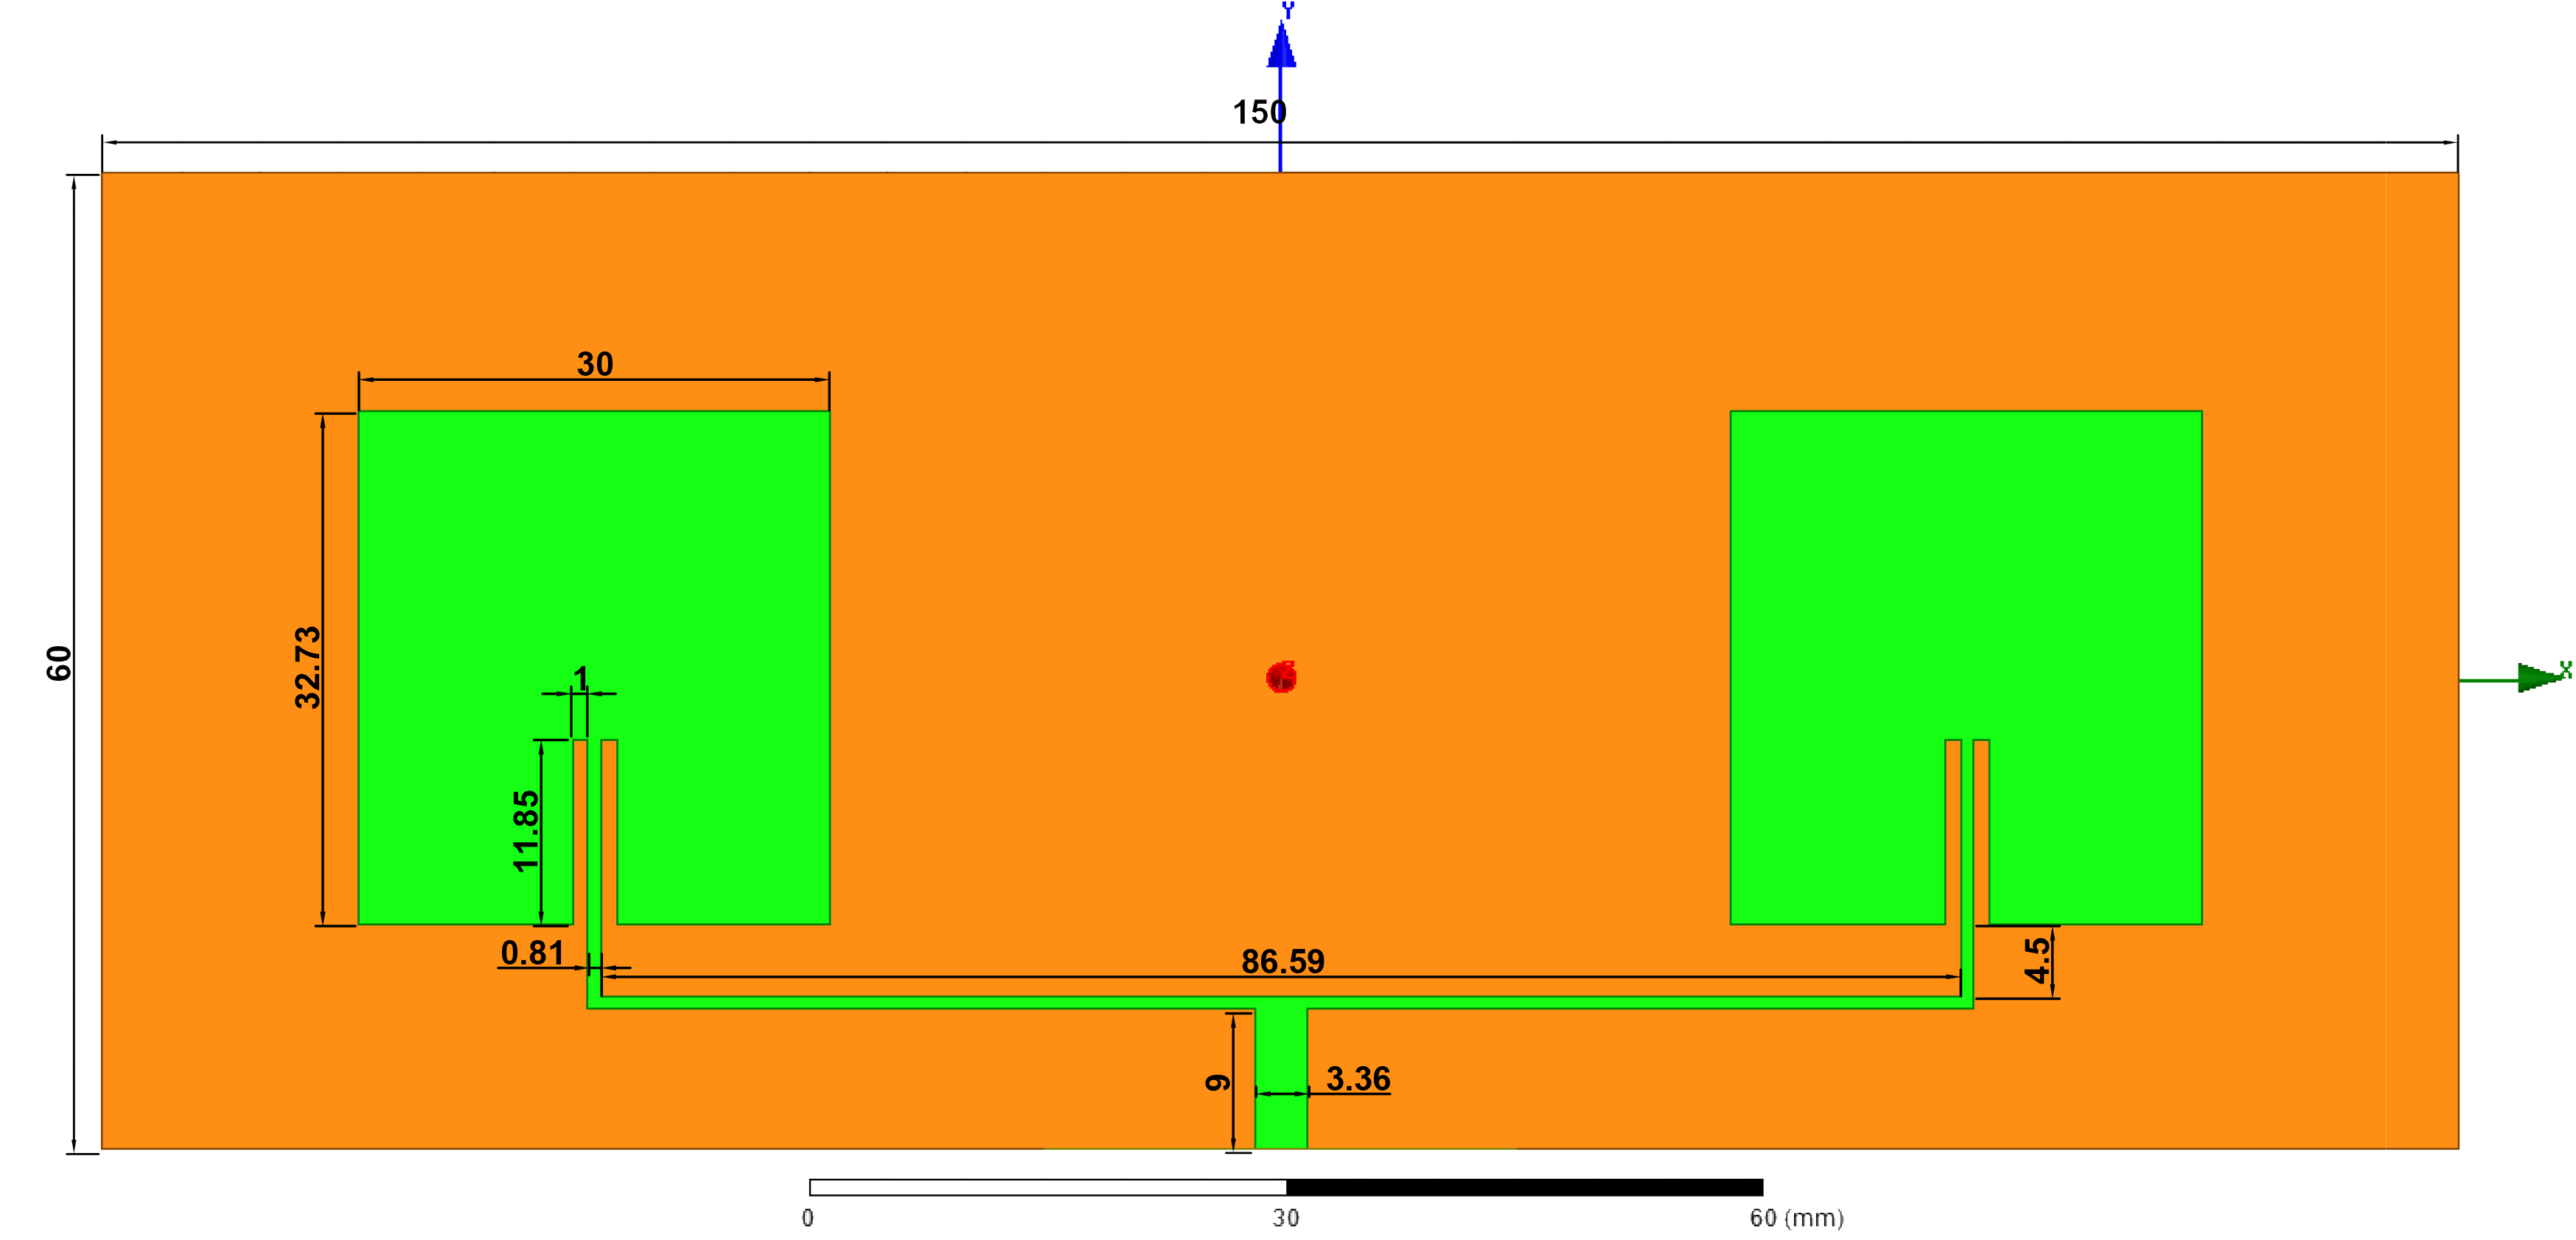
\includegraphics[width=14cm]{archivos/desarrollo/autocad/3}
        \caption{Array 2x1 en paralelo a 2.4 Ghz}
         \label{fig:array2x11}
\end{figure}

\begin{figure}[p]
    \centering
        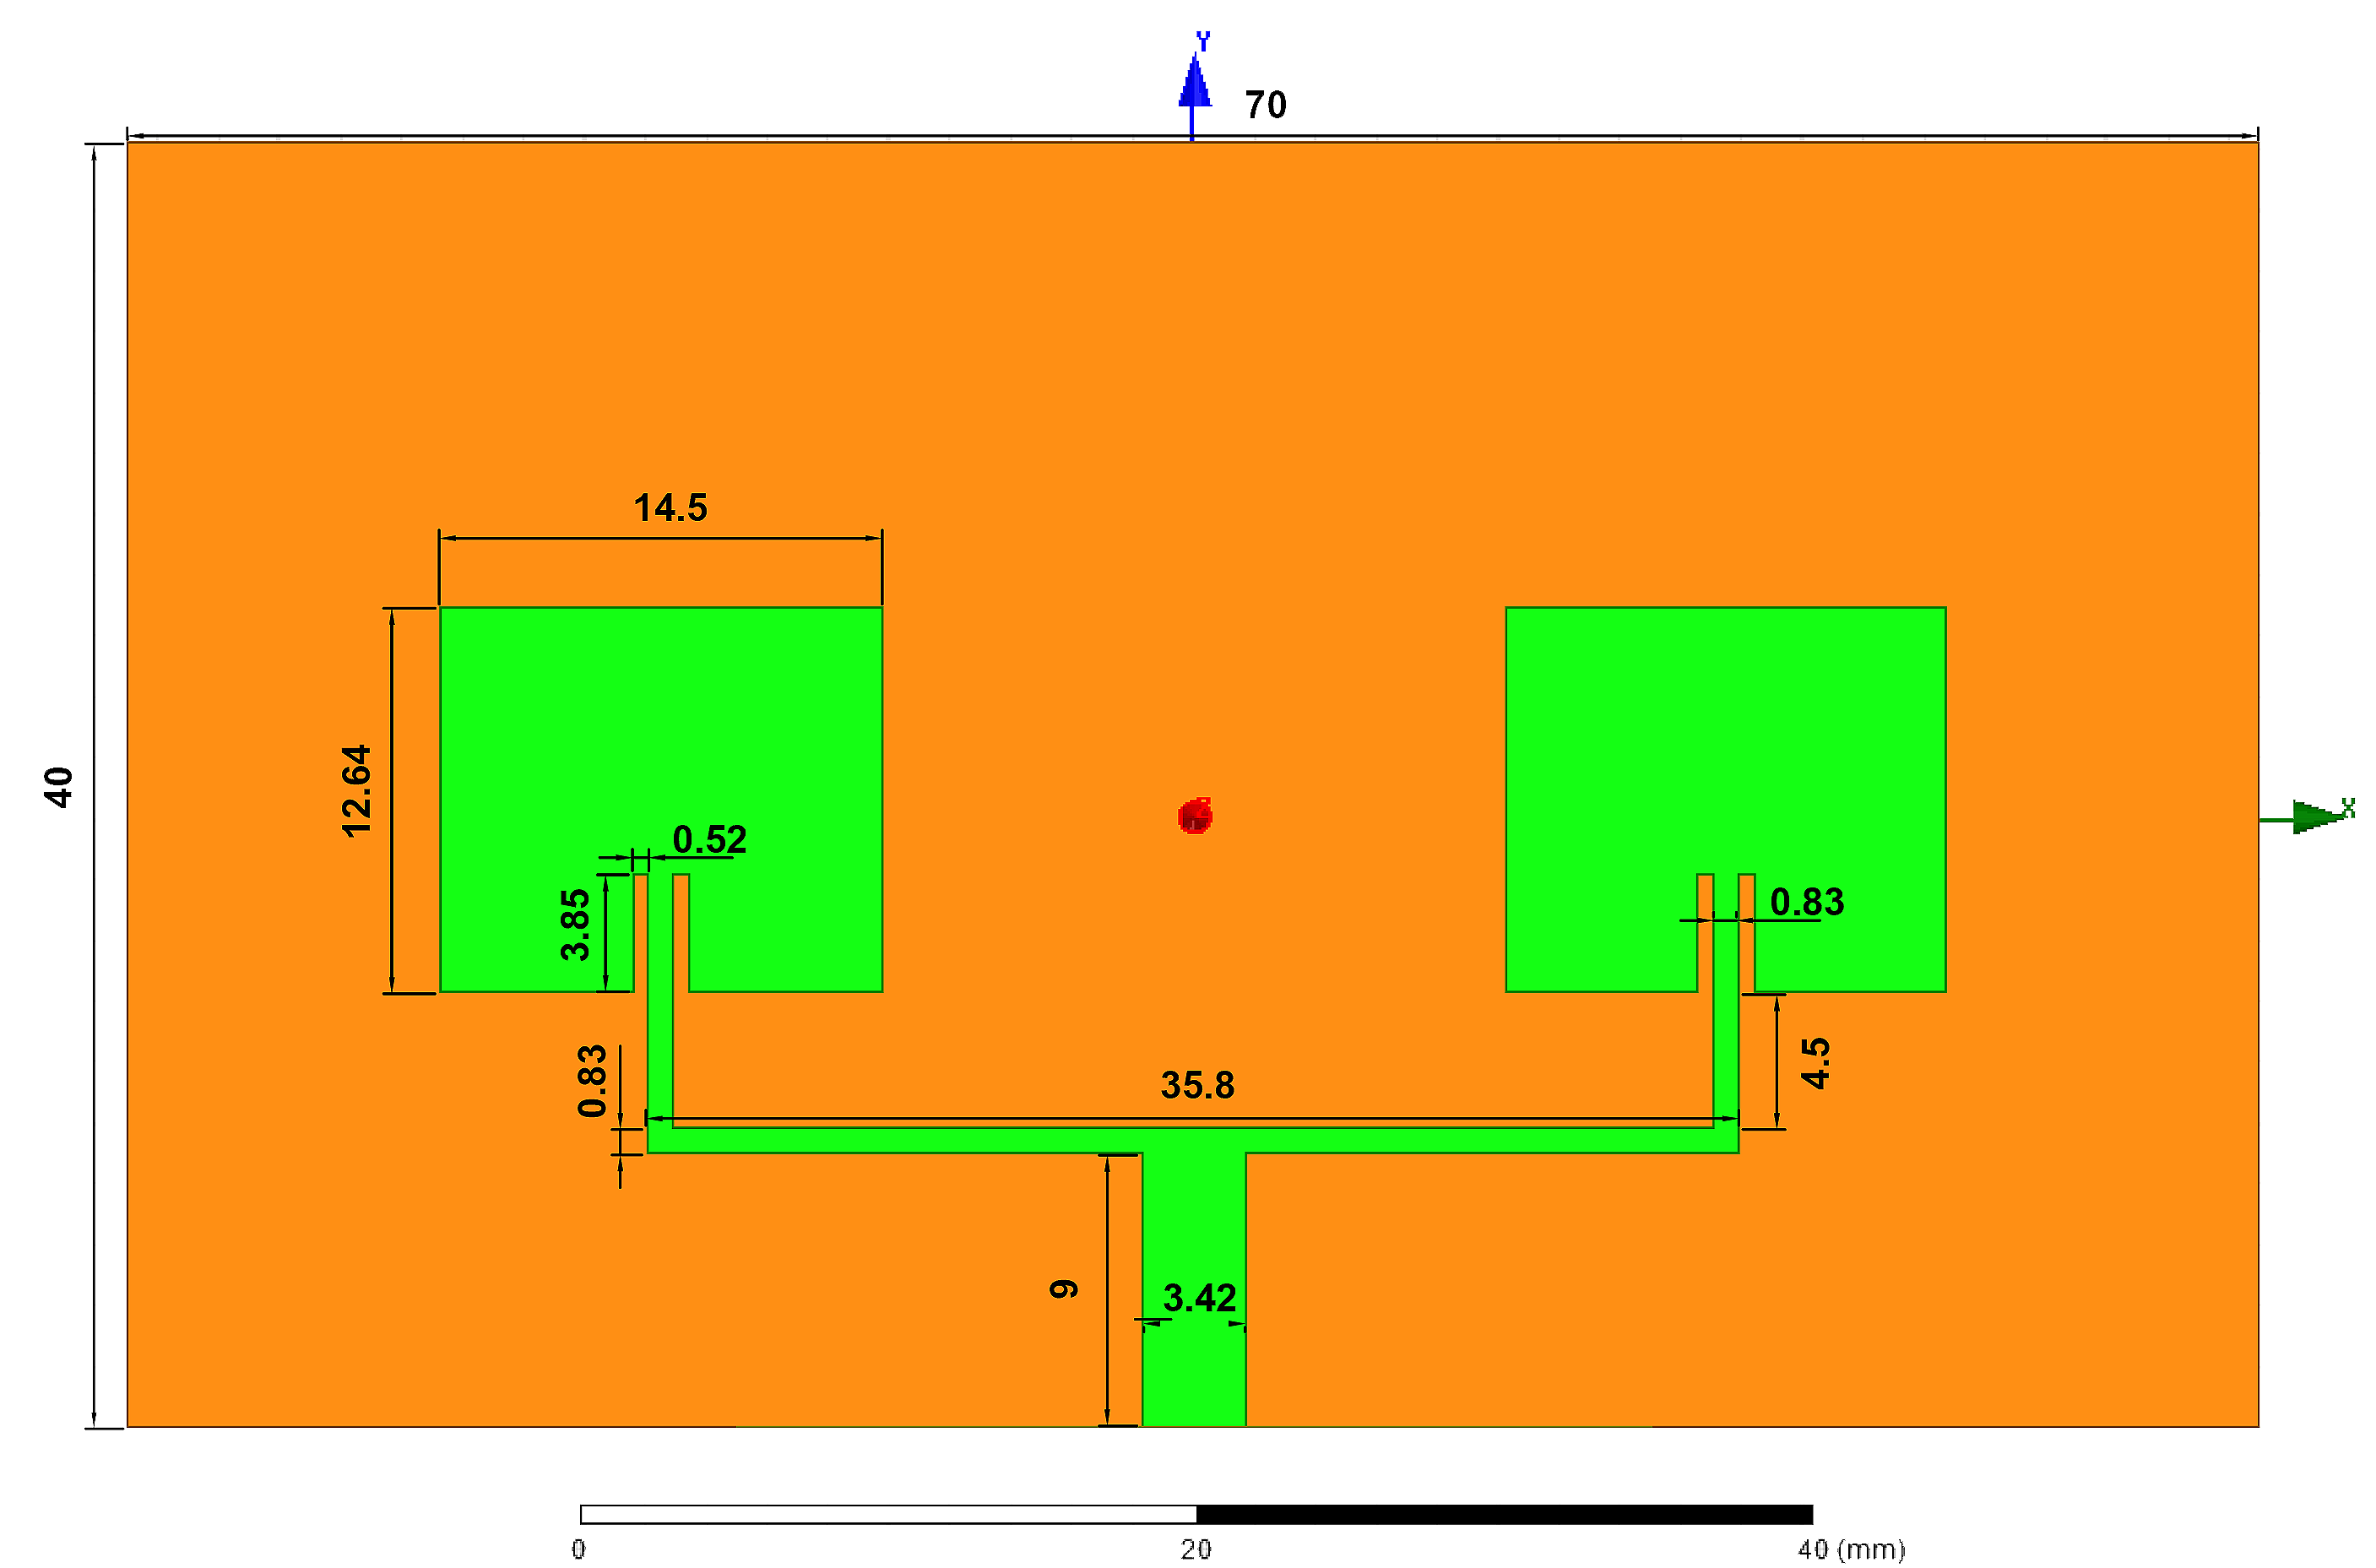
\includegraphics[width=14cm]{archivos/desarrollo/autocad/4}
        \caption{Array 2x1 en paralelo a 6 Ghz}
         \label{fig:array2x12}
\end{figure}

\newpage





\subsubsection{Array 2x1 Serie} 
\par POR HACER




\subsubsection{Array 2x2 Paralelo} 
\par HACIENDO

\begin{table}[h]
  
   \label{tab:array2x21}
   \small % text size of table content
   \centering % center the table
   \begin{tabular}{m{0.2\linewidth}m{0.25\linewidth}m{0.25\linewidth}} % alignment of each column data
   \toprule[\heavyrulewidth]\toprule[\heavyrulewidth]
   \textbf{Parámetro} & \textbf{Dimensión MATLAB} & \textbf{Dimensión final} \\ 
   \midrule
   \textbf{W} & 41.40 mm & 30.5 mm \\
   \textbf{L} & 32.73 mm & 32.29 mm\\
   \textbf{Linset} & 11.89 mm & 11.89 mm\\
   \textbf{Winset} & - & 1 mm\\
   \textbf{W50} & 3.36 mm & 2.84 mm\\
   \textbf{W70} & 1.85 mm & 1.81 mm\\
   \textbf{W100} & 0.85 mm & 0.81 mm\\
   \textbf{Ws/Ls} & - & 200/150 mm\\
   \textbf{Llambdacuartos} & 17.09 mm & 17.09 mm\\
   \bottomrule[\heavyrulewidth] 
   \end{tabular}
   \caption{Dimensiones de array 2x1 microstrip a 2.4 GHz} 
\end{table}


\begin{table}[h]
  
   \label{tab:array2x22}
   \small % text size of table content
   \centering % center the table
   \begin{tabular}{m{0.2\linewidth}m{0.25\linewidth}m{0.25\linewidth}} % alignment of each column data
   \toprule[\heavyrulewidth]\toprule[\heavyrulewidth]
   \textbf{Parámetro} & \textbf{Dimensión MATLAB} & \textbf{Dimensión final} \\ 
   \midrule
   \textbf{W} & 16.56 mm & 15.2 mm \\
   \textbf{L} & 12.64 mm & 12.5 mm\\
   \textbf{Linset} & 4.57 mm & 3.31 mm\\
   \textbf{Winset} & - & 0.5 mm\\
   \textbf{W50} & 3.34 mm & 3.42 mm\\
   \textbf{W70} & 3.34 mm & 1.83 mm\\
   \textbf{W100} & 0.85 mm & 0.83 mm\\
   \textbf{Ws/Ls} & - mm & 70/65 mm\\
   \bottomrule[\heavyrulewidth] 
   \end{tabular}
   \caption{Dimensiones de array 2x1 microstrip a 6 GHz} 
\end{table}

\begin{figure}[p]
    \centering
        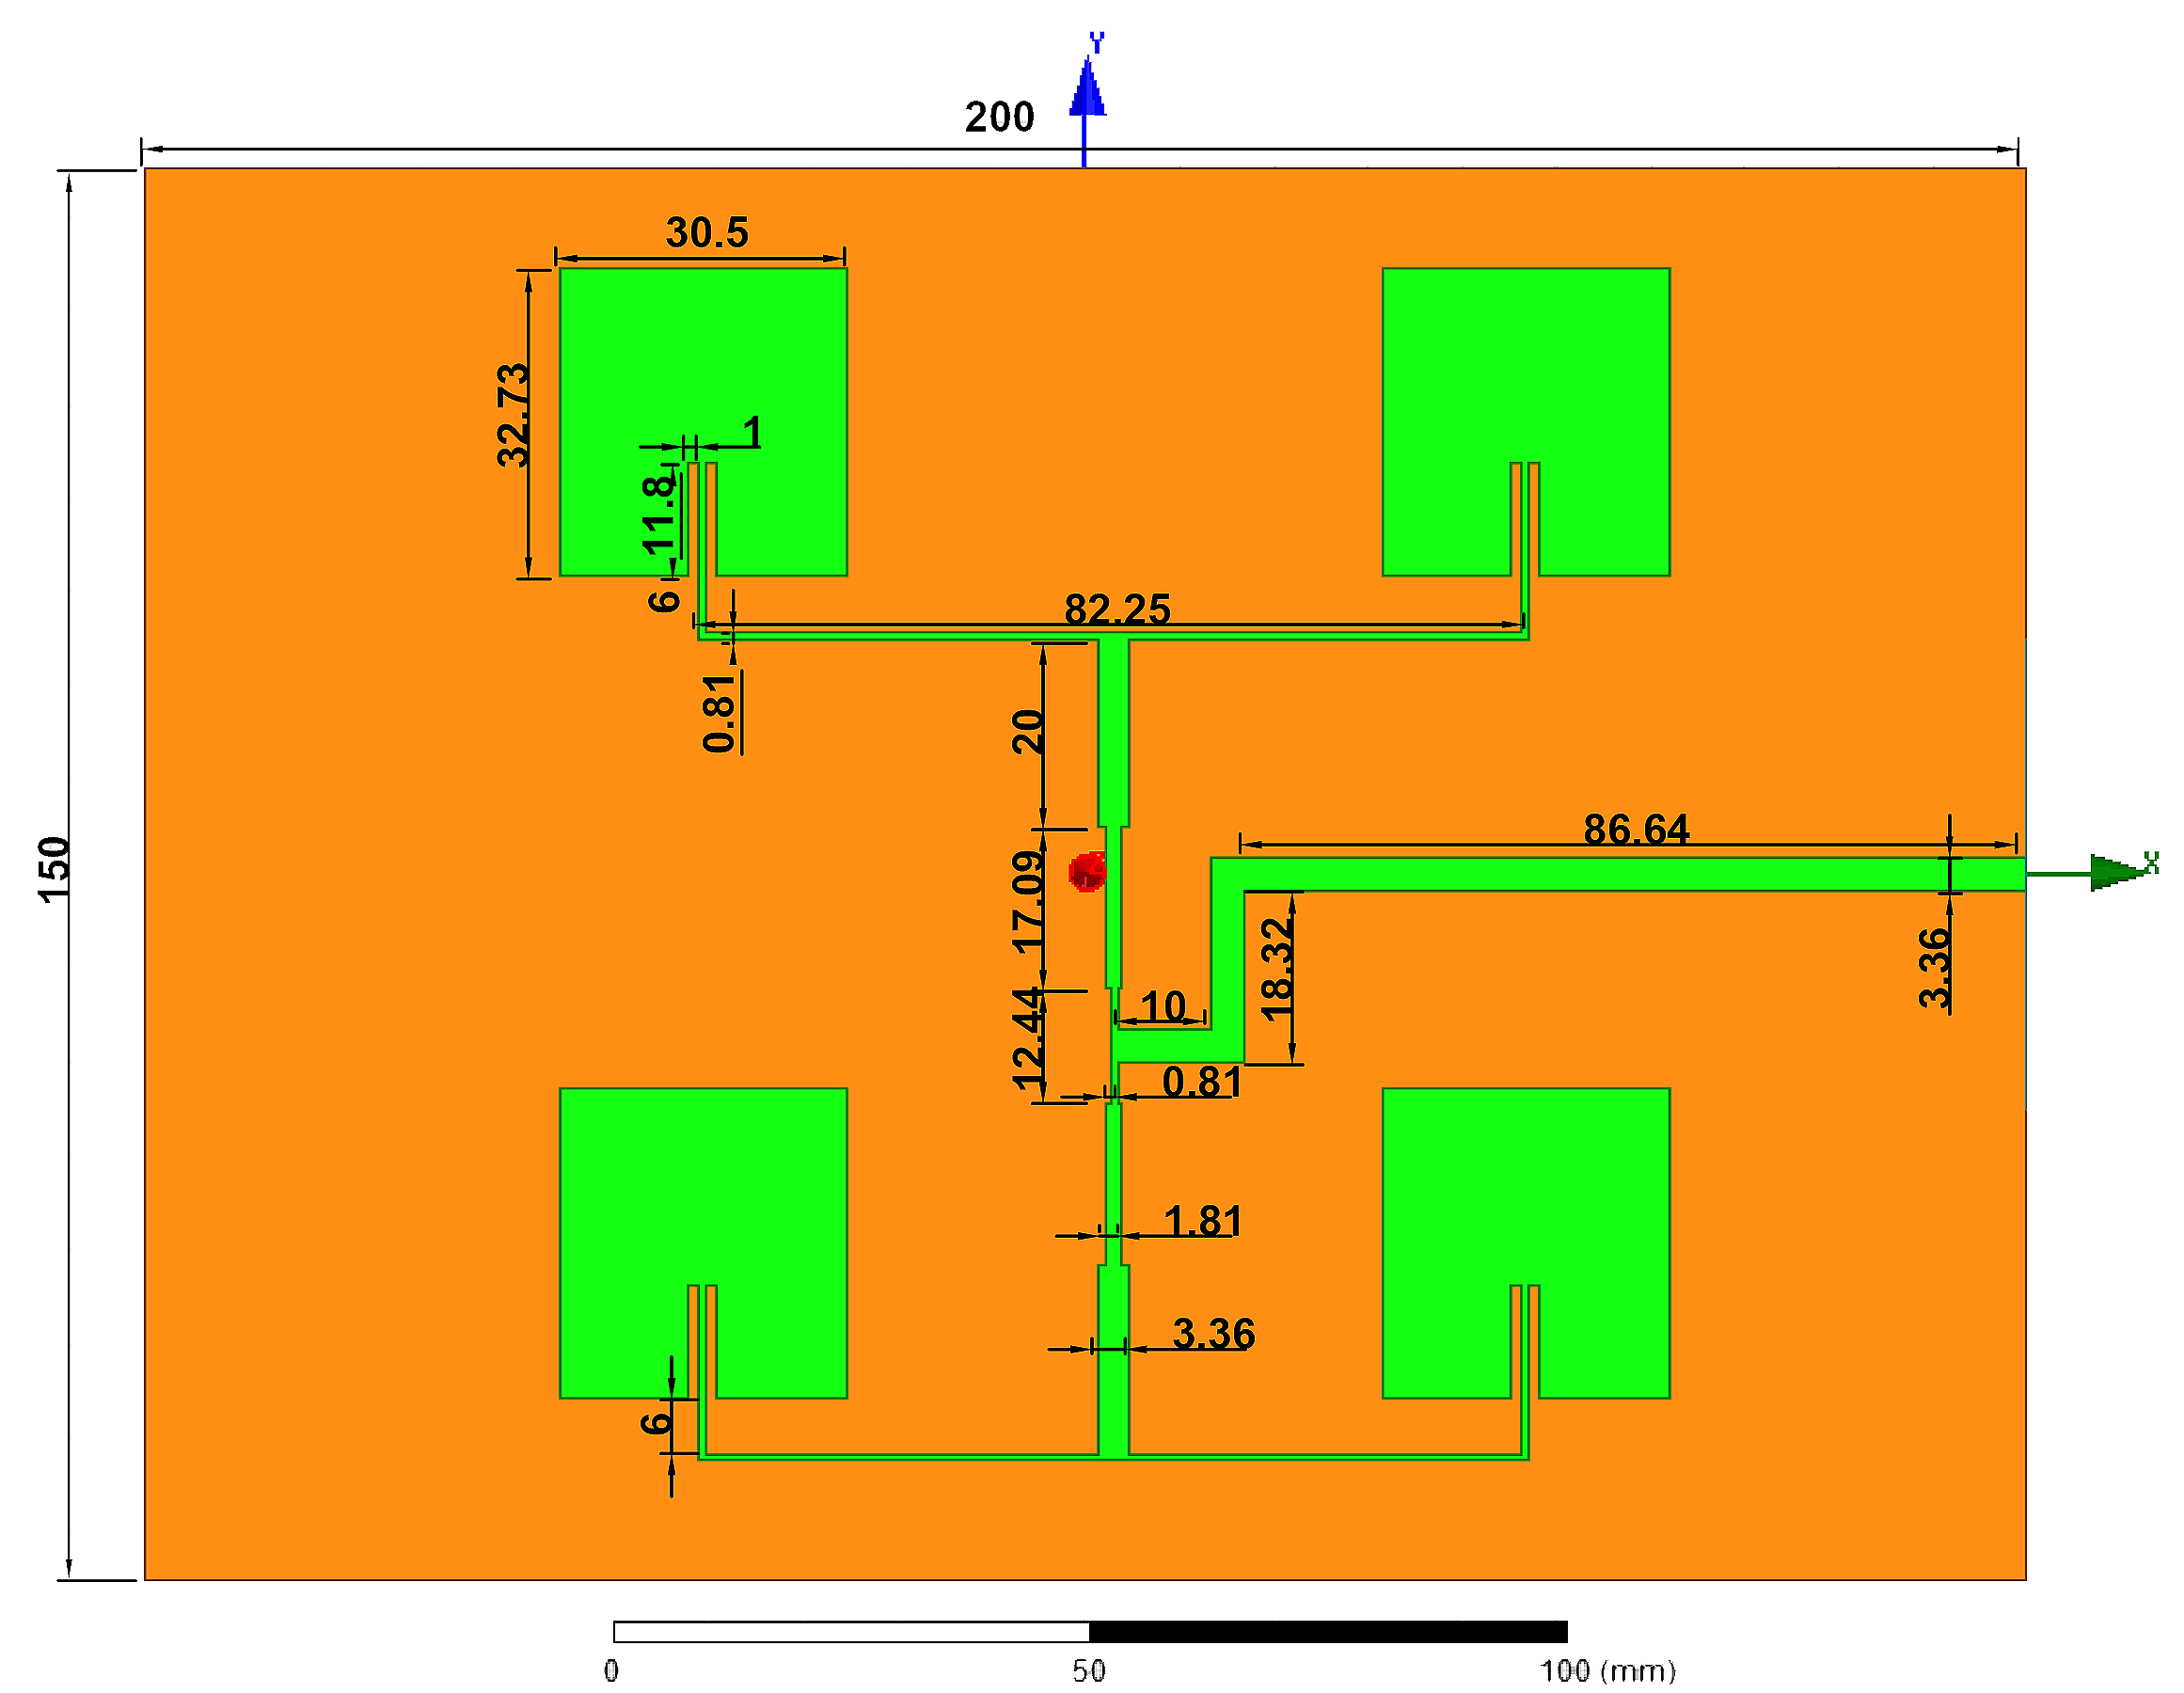
\includegraphics[width=12cm]{archivos/desarrollo/autocad/7}
        \caption{Array 2x2 en paralelo a 2.4 Ghz}
         \label{fig:array2x21}
\end{figure}

\begin{figure}[p]
    \centering
        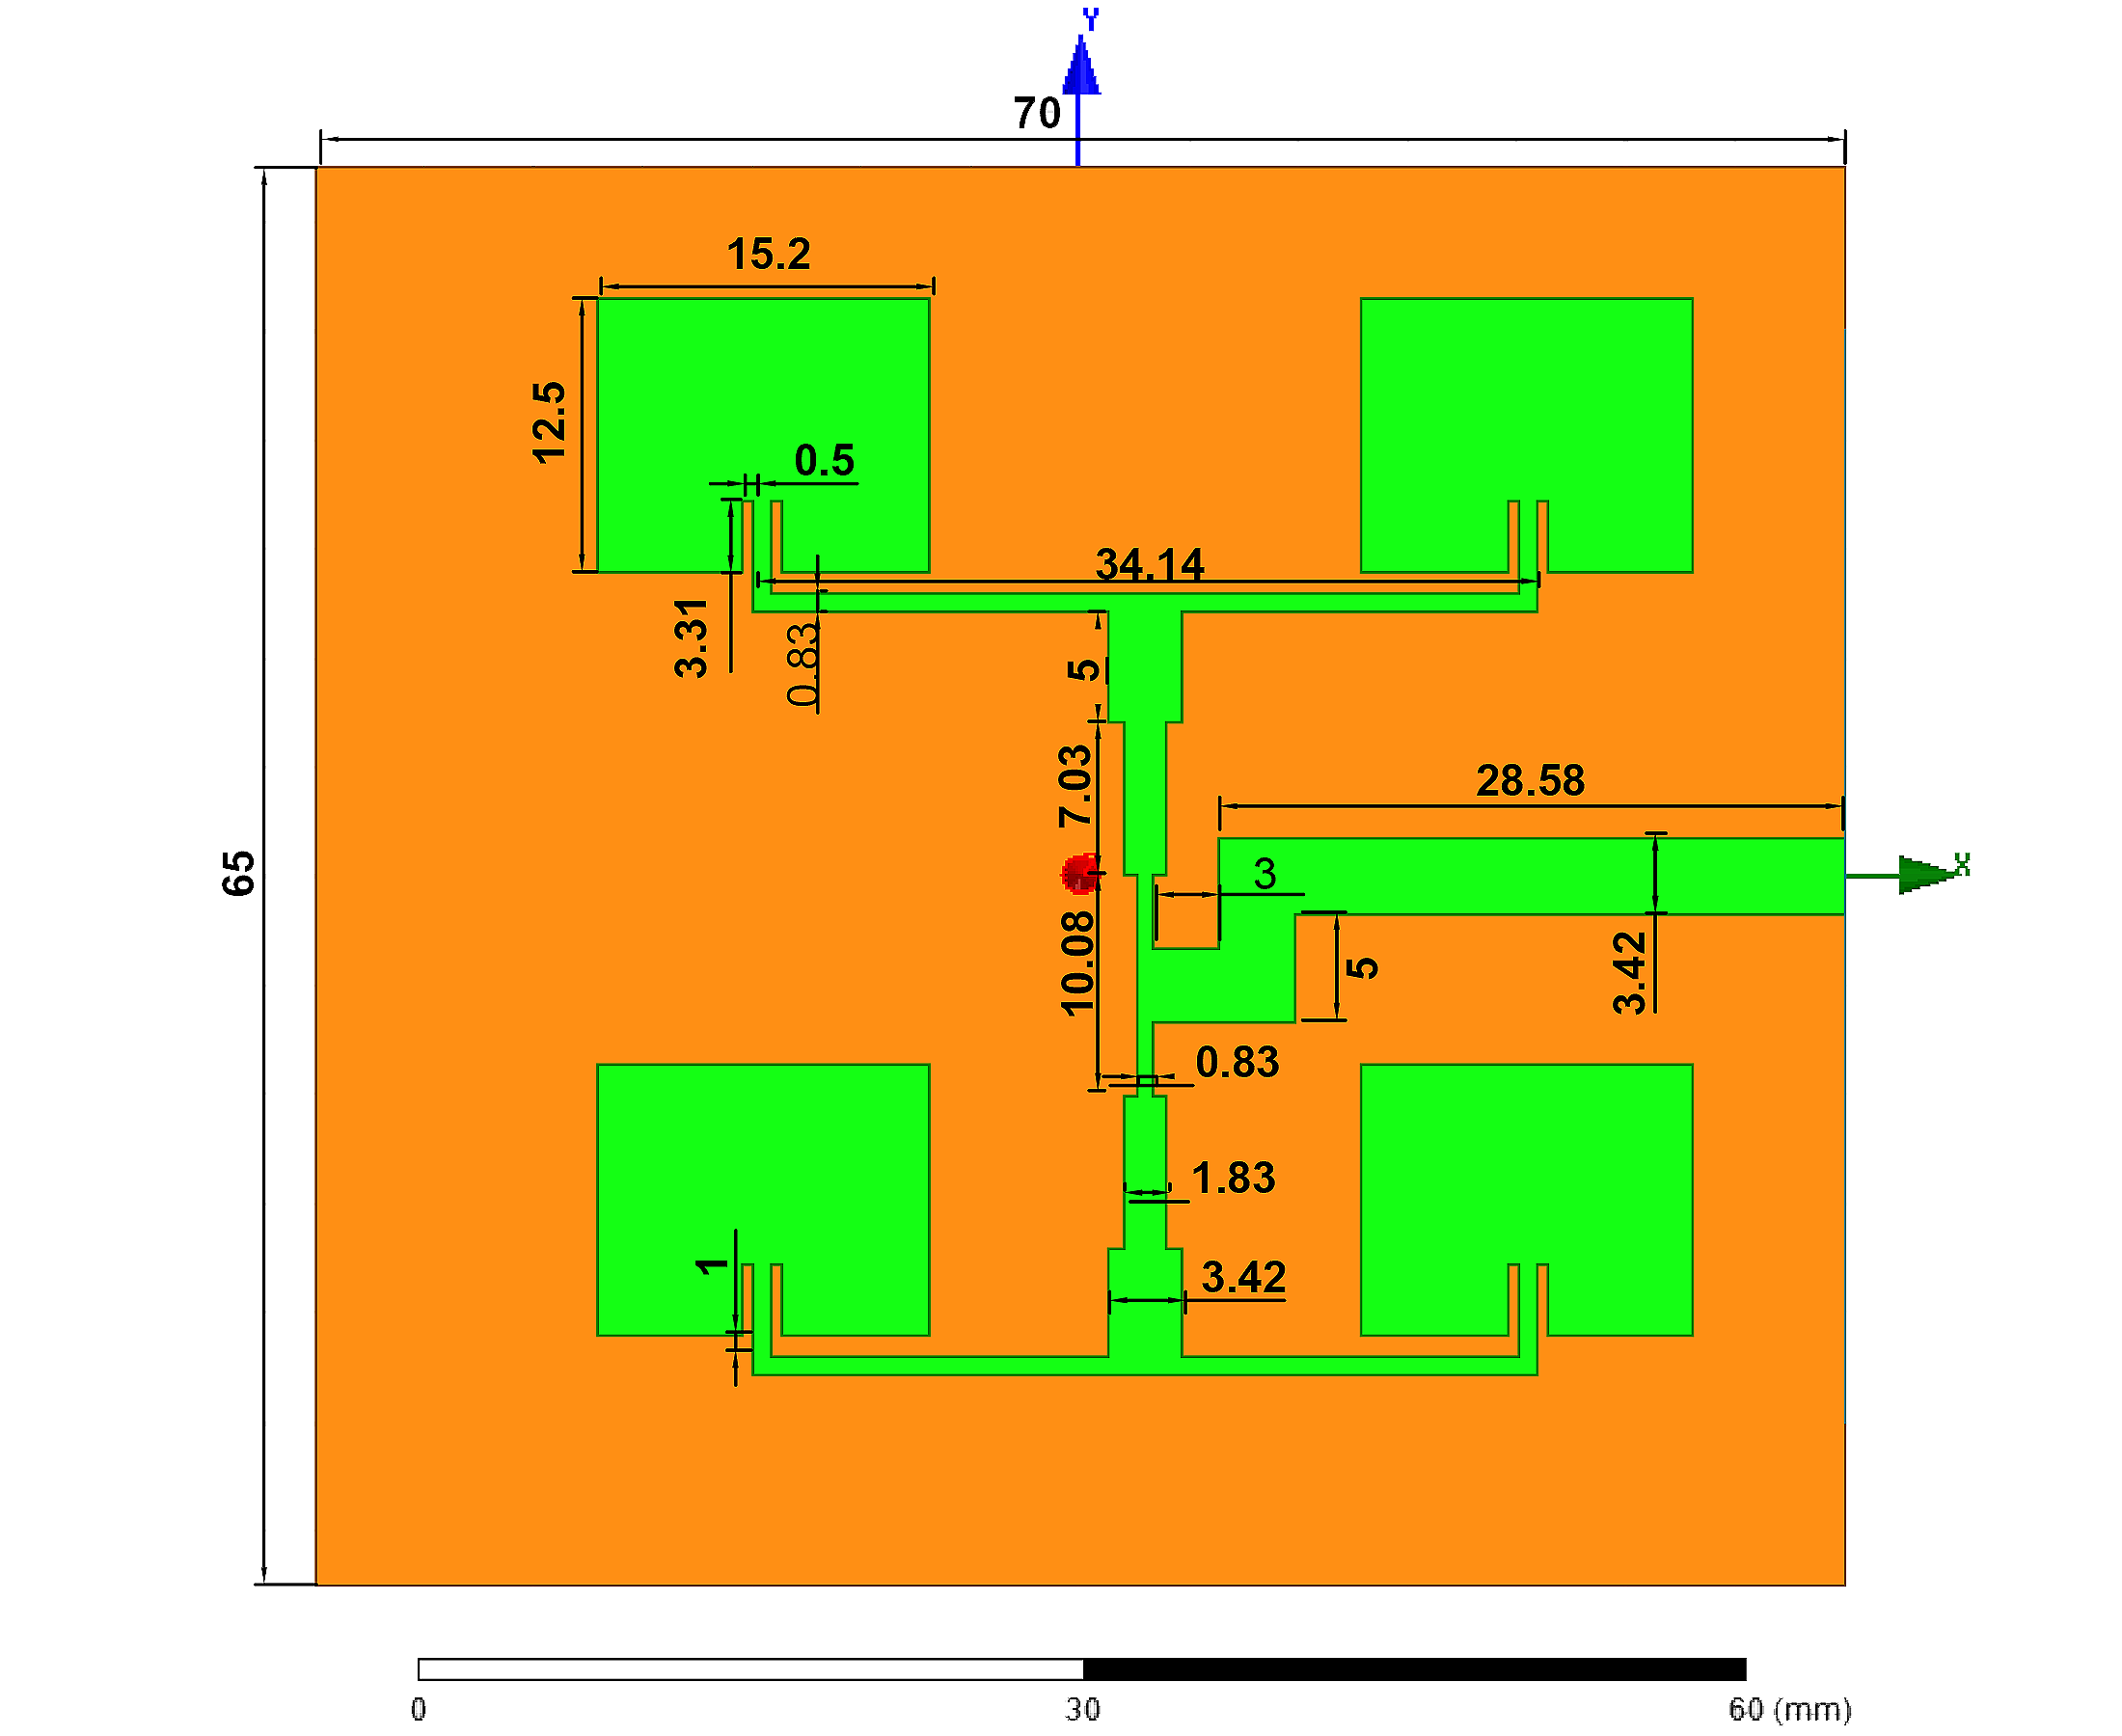
\includegraphics[width=12cm]{archivos/desarrollo/autocad/8}
        \caption{Array 2x2 en paralelo a 6 Ghz}
         \label{fig:array2x22}
\end{figure}

\newpage



\subsubsection{Array 4x1 Paralelo} 
\par La antena microtrip simple de un único parche ha sido la antena estudiada en la sección anterior para el caso de 2.4 Ghz. Se trata de una antena muy simple, alimentada mediante una línea microstrip directa cuya impedancia está referenciada a 50 $\Omega$.

\begin{table}[h]
  
   \label{tab:array4x11}
   \small % text size of table content
   \centering % center the table
   \begin{tabular}{m{0.2\linewidth}m{0.25\linewidth}m{0.25\linewidth}} % alignment of each column data
   \toprule[\heavyrulewidth]\toprule[\heavyrulewidth]
   \textbf{Parámetro} & \textbf{Dimensión MATLAB} & \textbf{Dimensión final} \\ 
   \midrule
   \textbf{W} & 41.40 mm & 43.56 mm \\
   \textbf{L} & 32.73 mm & 35.97 mm\\
   \textbf{Linset} & 11.89 mm & 9.8 mm\\
   \textbf{Winset} & - & 1.08 mm\\
   \textbf{W50} & 3.36 mm & 4.2 mm\\
   \textbf{W100} & 0.85 mm & 2 mm\\
   \textbf{Ws/Ls} & - mm & 100/70 mm\\
   \bottomrule[\heavyrulewidth] 
   \end{tabular}
   \caption{Dimensiones de array 2x1 microstrip a 2.4 GHz} 
\end{table}

\begin{table}[h]
  
   \label{tab:array4x12}
   \small % text size of table content
   \centering % center the table
   \begin{tabular}{m{0.2\linewidth}m{0.25\linewidth}m{0.25\linewidth}} % alignment of each column data
   \toprule[\heavyrulewidth]\toprule[\heavyrulewidth]
   \textbf{Parámetro} & \textbf{Dimensión MATLAB} & \textbf{Dimensión final} \\ 
   \midrule
   \textbf{W} & 16.56 mm & 14.5 mm \\
   \textbf{L} & 12.64 mm & 12.64 mm\\
   \textbf{Linset} & 4.57 mm & 3.85 mm\\
   \textbf{Winset} & - & 0.52 mm\\
   \textbf{W50} & 3.34 mm & 3.42 mm\\
   \textbf{W100} & 0.85 mm & 0.83 mm\\
   \textbf{Ws/Ls} & - mm & 70/40 mm\\
   \bottomrule[\heavyrulewidth] 
   \end{tabular}
   \caption{Dimensiones de array 2x1 microstrip a 6 GHz} 
\end{table}

\begin{figure}[p]
    \centering
        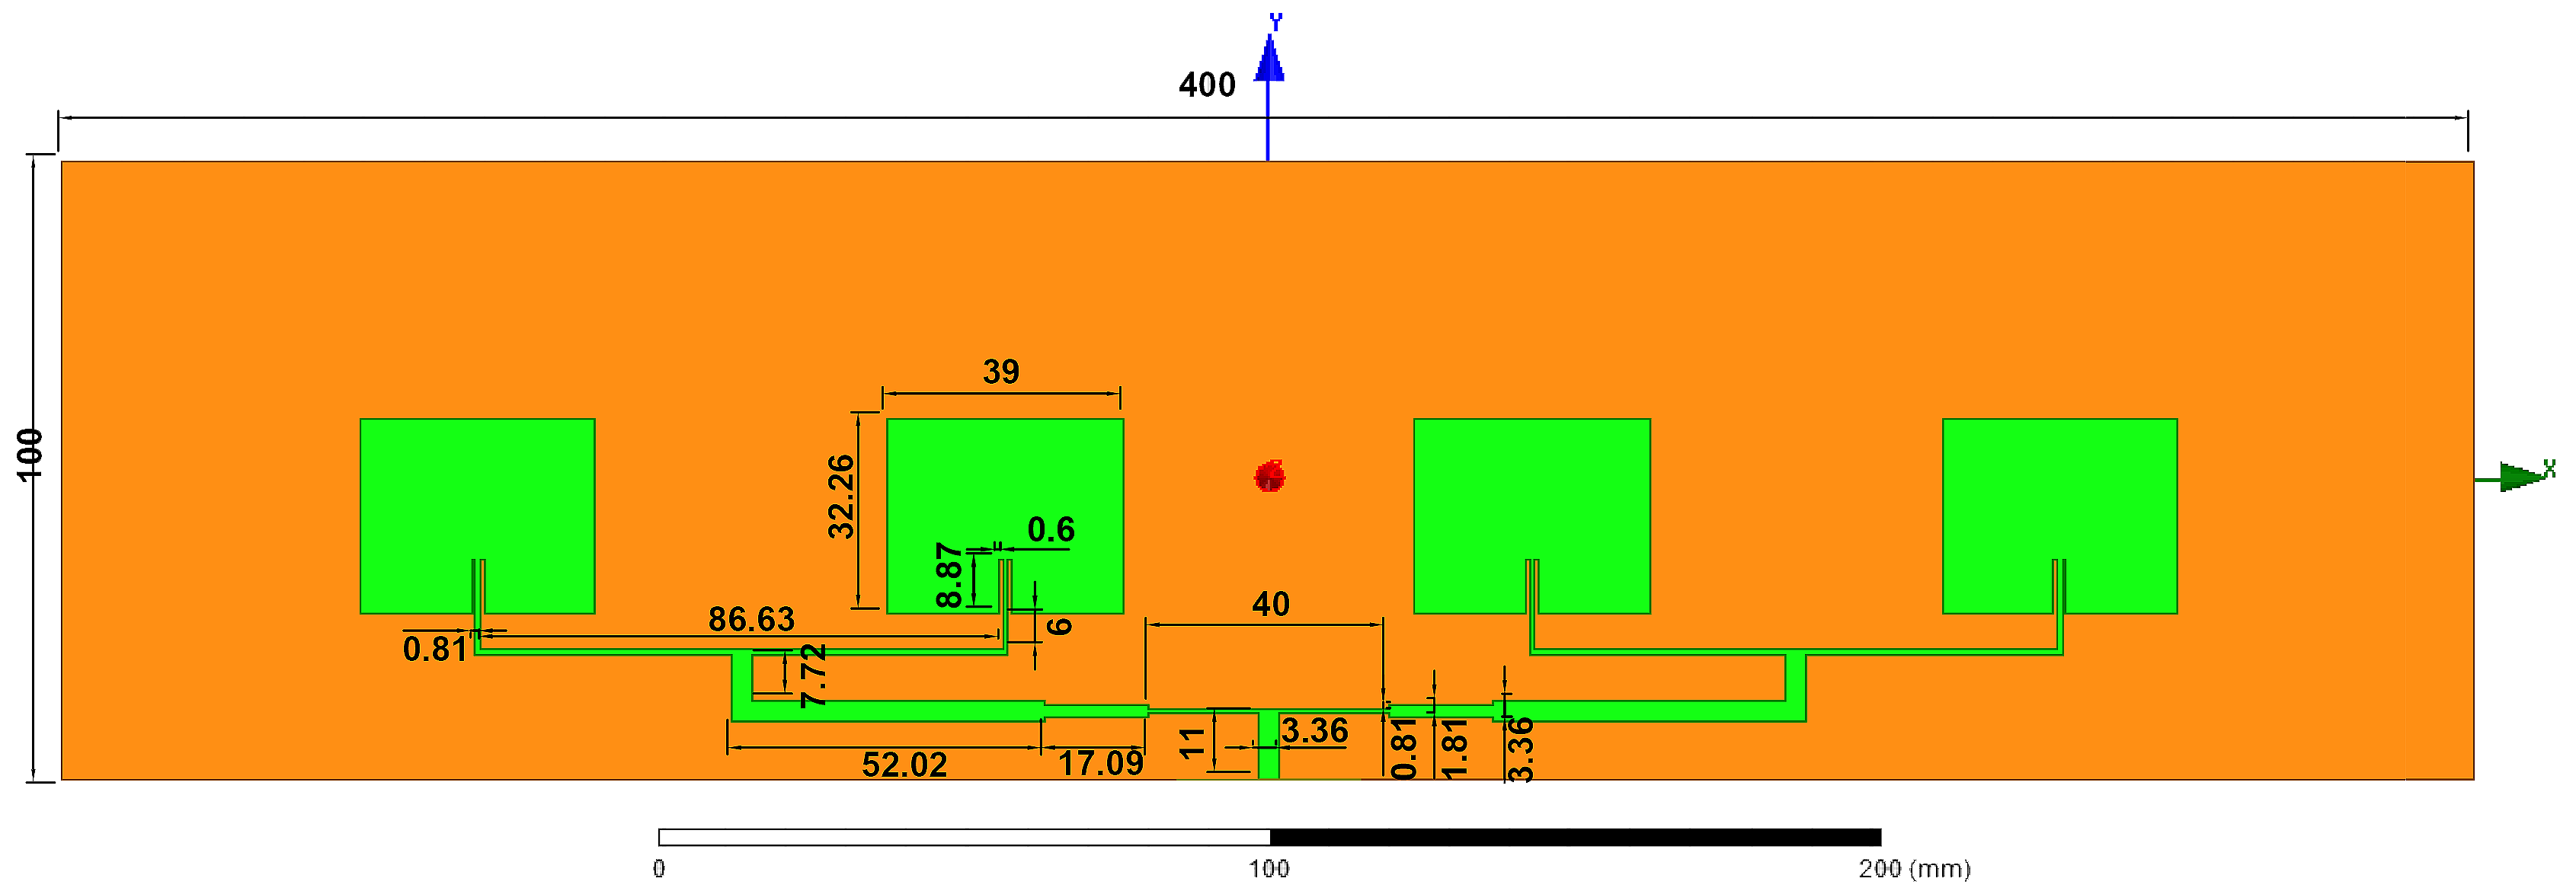
\includegraphics[width=14cm]{archivos/desarrollo/autocad/5}
        \caption{Array 2x2 en paralelo a 2.4 Ghz}
         \label{fig:array4x11}
\end{figure}

\begin{figure}[p]
    \centering
        \includegraphics[width=14cm]{archivos/desarrollo/autocad/6}
        \caption{Array 2x2 en paralelo a 6 Ghz}
         \label{fig:array4x12}
\end{figure}




\subsubsection{Array 4x2 Paralelo} 
\par La antena microtrip simple de un único parche ha sido la antena estudiada en la sección anterior para el caso de 2.4 Ghz. Se trata de una antena muy simple, alimentada mediante una línea microstrip directa cuya impedancia está referenciada a 50 $\Omega$.

\subsubsection{Array 4x4 Paralelo} 
\par La antena microtrip simple de un único parche ha sido la antena estudiada en la sección anterior para el caso de 2.4 Ghz. Se trata de una antena muy simple, alimentada mediante una línea microstrip directa cuya impedancia está referenciada a 50 $\Omega$.		% Plantilla: Se muestran listados
%\chapter{Análisis de los resultados}
\label{resultados}

A lo largo de este capitulo se va a tratar de analizar, comparar y discutir los resultados obtenidos mediante HFSS sobre los diseños que se comentaron en la sección \ref{analdis}. Se analizará cada configuración por separado y se mostrarán las gráficas y valores principales para cada una de las configuraciones de 2GHz y 6 GHz y finalmente la configuración a 27 GHz. No se analizará el caso del parche simple a 2.4 GHz puesto que ya fue analizado detalladamente en la sección \ref{procesodiseno}.

\section{Parche Simple a 6 GHz}
\par Para el parche simple a 6 GHz los resultados obtenidos son los siguientes:

\subsection{Pérdidas de retorno}
\par Comenzaremos analizando la curva de pérdidas de retorno o parámetro S del parche simple a 6 GHz, donde se puede observar un valor pico de -40.35 dB y un ancho de banda de 168 MHz, desde los 5.917 GHz hasta los 6.086 GHz, lo que equivale a un 2.81\% de la frecuencia de trabajo.
\\
\begin{figure}[H]
    \centering
        \includegraphics[width=\textwidth]{archivos/analisis/1x12/1}
        \caption{Parámetro S para el parche simple a 6 GHz}
        \label{fig:s1x12}
\end{figure}

\subsection{Reactancia}
\par La curva de reactancia arroja un valor a la frecuencia de trabajo de -0.63 $\Omega$. Muy cerca del valor esperado, 0.
\\
\begin{figure}[H]
    \centering
        \includegraphics[width=0.85\textwidth]{archivos/analisis/1x12/2}
        \caption{Reactancia para el parche simple a 6 GHz}
        \label{fig:react1x12}
\end{figure}


\subsection{Resistencia}
\par La parte real de la impedancia ofrece un valor a la frecuencia de trabajo de 49.28 $\Omega$. Muy cerca del valor esperado, 50, con un error de tan solo el 1.44\%.
\\
\begin{figure}[H]
    \centering
        \includegraphics[width=0.85\textwidth]{archivos/analisis/1x12/3}
        \caption{Resistencia para el parche simple a 6 GHz}
        \label{fig:resis1x12}
\end{figure}


\subsection{Patrón de radiación}
\par En cuanto a los patrones de radiación, se puede observar como, al igual que el parche simple a 2.4 GHz, el patrón de radiación es omnidireccional para el plano superior de la antena, y no se ve afectado por ningún otro tipo de elemento radiante. La directividad para el ángulo de máxima radiación encontrada es de 7.66 dB.
\\
\subsubsection{Plano E}
\begin{figure}[H]
    \centering
        \includegraphics[width=0.8\textwidth]{archivos/analisis/1x12/4}
        \caption{Radiación en el plano E para el parche simple a 6 GHz}
        \label{fig:E1x12}
\end{figure}

\subsubsection{Plano H}
\begin{figure}[H]
    \centering
        \includegraphics[width=0.8\textwidth]{archivos/analisis/1x12/5}
        \caption{Radiación en el plano H para el parche simple a 6 GHz}
        \label{fig:H1x12}
\end{figure}

\newpage
\subsection{Radiación 3D}
\par Mediante el diagrama de radiación 3D se puede observar el comportamiento omnidireccional de la antena. 

\begin{figure}[H]
     \centering
     \begin{subfigure}[b]{0.75\textwidth}
         \centering
         \includegraphics[width=0.85\textwidth]{archivos/analisis/1x12/6}
         \caption{Representación isométrica del diagrama de radiación 3D}
         \label{fig:3d11x12}
     \end{subfigure}
     \hfill
     \begin{subfigure}[b]{0.75\textwidth}
         \centering
         \includegraphics[width=0.85\textwidth]{archivos/analisis/1x12/7}
         \caption{Representación superior del diagrama de radiación 3D}
         \label{fig:3d21x12}
     \end{subfigure}
     \hfill
        \caption{Radiación 3D para el parche simple a 6 GHz}
        \label{fig:3d1x12}
\end{figure}

\newpage
\subsection{Campo eléctrico}
\par Finalmente, podemos observar la distribución de campos eléctricos en el parche. 

\begin{figure}[H]
    \centering
        \includegraphics[width=\textwidth]{archivos/analisis/1x12/8}
        \caption{Distribución de campos eléctricos para el parche simple a 6 GHz}
        \label{fig:elec1x12}
\end{figure}


\subsection{Resumen}
\par Como se puede observar en este parche único a 6 GHz, los resultados obtenidos son muy similares a los obtenidos en el caso de 2.4 GHz. El patrón de radiación de la antena se caracteriza por el ser el más básico que podemos encontrar en una antena de tipo microstrip, además de tratarse de un patrón muy útil para aplicaciones móviles puesto que su característica omnidireccional se adapta a los casos de uso en los que el patrón de radiación de la antena no esté apuntando directamente a la antena de telefonía. 
\\
\par En la tabla \ref{tab:1x12} se pueden observar un resumen de los parámetros característicos de la antena. En ella se puede observar el buen rendimiento obtenido

\begin{table}[H]
  
   \label{tab:1x12}
   \small % text size of table content
   \centering % center the table
   \begin{tabular}{m{0.4\linewidth}m{0.4\linewidth}} % alignment of each column data
   \toprule[\heavyrulewidth]\toprule[\heavyrulewidth]
   \textbf{Parámetro} & \textbf{Parche simple 6 GHz} \\ 
   \midrule
   \textbf{S(1,1)} & -40.35 dB \\
   \textbf{Ancho de banda} & 168 MHz dB \\
   \textbf{Directividad} & 7.66 dB \\
   \textbf{Ganancia} & 7.41 dB \\
   \textbf{Eficiencia de radiación} & 93.15\% \\
   \textbf{Relación delante/atrás} & 18.42 dB \\

   \bottomrule[\heavyrulewidth] 
   \end{tabular}
   \caption{Parámetros característicos del parche único microstrip a 6 GHz} 
\end{table}









\section{Array 2x1 a 2.4 GHz}
\par Para el array en configuración 2x1 a 2.4 GHz los resultados obtenidos son los siguientes:

\subsection{Pérdidas de retorno}
\par En cuanto a su curva de pérdidas de retorno del array a 2.4 GHz, se puede observar un valor pico de -36.46 dB y un ancho de banda de 34.3 MHz, desde los 2.3835 GHz hasta los 2.4173 GHz, lo que equivale a un 1.43\% de la frecuencia de trabajo.
\\
\begin{figure}[H]
    \centering
        \includegraphics[width=\textwidth]{archivos/analisis/2x11/1}
        \caption{Parámetro S para el array 2x1 a 2.4 GHz}
        \label{fig:s2x11}
\end{figure}

\subsection{Reactancia}
\par La curva de reactancia arroja un valor a la frecuencia de trabajo de -1.37 $\Omega$. 
\\
\begin{figure}[H]
    \centering
        \includegraphics[width=0.85\textwidth]{archivos/analisis/2x11/2}
        \caption{Reactancia para el array 2x1 a 2.4 GHz}
        \label{fig:react2x11}
\end{figure}

\subsection{Resistencia}
\par La parte real de la impedancia ofrece un valor a la frecuencia de trabajo de 48.12 $\Omega$.
\\
\begin{figure}[H]
    \centering
        \includegraphics[width=0.85\textwidth]{archivos/analisis/2x11/3}
        \caption{Resistencia para el array 2x1 a 2.4 GHz}
        \label{fig:resis2x11}
\end{figure}

\subsection{Patrón de radiación}
\par En cuanto a los patrones de radiación, se puede observar se puede observar un comportamiento más directivo con unos lóbulos laterales y trasero de bastante magnitud en relación al lóbulo principal para el plano E, mientras que en el plano H se observa un comportamiento completamente omnidireccional para el plano superior del array. La directividad en el ángulo de máxima radiación observada es de 7.64 dB.
\\
\subsubsection{Plano E}
\begin{figure}[H]
    \centering
        \includegraphics[width=0.75\textwidth]{archivos/analisis/2x11/4}
        \caption{Radiación en el plano E para el array 2x1 a 2.4 GHz}
        \label{fig:E2x11}
\end{figure}

\subsubsection{Plano H}
\begin{figure}[H]
    \centering
        \includegraphics[width=0.75\textwidth]{archivos/analisis/2x11/5}
        \caption{Radiación en el plano H para el array 2x1 a 2.4 GHz}
        \label{fig:H2x11}
\end{figure}

\subsection{Radiación 3D}
\par Mediante el diagrama de radiación 3D se puede observar el comportamiento directivo en el plano perpendicular a la configuración del array, producido por la superposición de la radiación de ambos parches.

\begin{figure}[H]
     \centering
     \begin{subfigure}[b]{0.7\textwidth}
         \centering
         \includegraphics[width=0.85\textwidth]{archivos/analisis/2x11/6}
         \caption{Representación isométrica del diagrama de radiación 3D}
         \label{fig:3d12x11}
     \end{subfigure}
     \hfill
     \begin{subfigure}[b]{0.7\textwidth}
         \centering
         \includegraphics[width=0.85\textwidth]{archivos/analisis/2x11/7}
         \caption{Representación superior del diagrama de radiación 3D}
         \label{fig:3d22x11}
     \end{subfigure}
     \hfill
        \caption{Radiación 3D para el array 2x1 a 2.4 GHz}
        \label{fig:3d2x11}
\end{figure}

\subsection{Campo eléctrico}
\par Finalmente, podemos observar la distribución de campos eléctricos en el parche. 

\begin{figure}[H]
    \centering
        \includegraphics[width=\textwidth]{archivos/analisis/2x11/8}
        \caption{Distribución de campos eléctricos para el para el array 2x1 a 2.4 GHz}
        \label{fig:elec2x11}
\end{figure}

\subsection{Resumen}
\par En esta primera configuración de array a 2.4 GHz se puede observar los primeros comportamientos directivos producidos por la conjunción de diferentes parches en fase funcionando en la misma antena. 
\\
\par En la tabla \ref{tab:2x11} se pueden observar un resumen de los parámetros característicos de la antena. Como se puede observar, el rendimiento obtenido para esta antena es un tanto menor al obtenido previamente en las antenas de parche único y esto es principalmente debido a la complejidad del proceso de adaptación al aumentar el número de parches en las configuraciones de array.

\begin{table}[H]
  
   
   \small % text size of table content
   \centering % center the table
   \begin{tabular}{m{0.2\linewidth}m{0.25\linewidth}} % alignment of each column data
   \toprule[\heavyrulewidth]\toprule[\heavyrulewidth]
   \textbf{Parámetro} & \textbf{Array 2x1 a 2.4 GHz} \\ 
   \midrule
   \textbf{S(1,1)} & -36.46 dB \\
   \textbf{Ancho de banda} & 34.3 MHz dB \\
   \textbf{Directividad} & 7.64 dB \\
   \textbf{Ganancia} & 7.03 dB \\
   \textbf{Eficiencia de radiación} & 86.94\% \\
   \textbf{Relación delante/atrás} & 15.89 dB \\

   \bottomrule[\heavyrulewidth] 
   \end{tabular}
   \label{tab:2x11}
   \caption{Parámetros característicos para el array 2x1 a 2.4 GHz} 
\end{table}













\section{Array 2x1 a 6 GHz}
\par Para el array en configuración 2x1 a 6 GHz los resultados obtenidos son los siguientes:

\subsection{Pérdidas de retorno}
\par En cuanto a su curva de pérdidas de retorno del array a 6 GHz, se puede observar un valor pico de -76.78 dB y un ancho de banda de 179.1 MHz, desde los 5.9014 GHz hasta los 6.0805 GHz, lo que equivale a un 2.98\% de la frecuencia de trabajo.
\\
\begin{figure}[H]
    \centering
        \includegraphics[width=\textwidth]{archivos/analisis/2x12/1}
        \caption{Parámetro S para el array 2x1 a 6 GHz}
        \label{fig:s2x12}
\end{figure}

\newpage
\subsection{Reactancia}
\par La curva de reactancia arroja un valor a la frecuencia de trabajo de -0.03 $\Omega$. 
\\
\begin{figure}[H]
    \centering
        \includegraphics[width=0.85\textwidth]{archivos/analisis/2x12/2}
        \caption{Reactancia para el array 2x1 a 6 GHz}
        \label{fig:react2x12}
\end{figure}

\subsection{Resistencia}
\par La parte real de la impedancia ofrece un valor a la frecuencia de trabajo de 49.35 $\Omega$.
\\
\begin{figure}[H]
    \centering
        \includegraphics[width=0.85\textwidth]{archivos/analisis/2x12/3}
        \caption{Resistencia para el array 2x1 a 6 GHz}
        \label{fig:resis2x12}
\end{figure}

\subsection{Patrón de radiación}
\par En este caso se puede observar el mismo patrón de radiación base que se encontró en el array 2x1 a 2.4 GHz pero con una directividad aumentada del lóbulo principal con respecto a los lóbulos secundarios y traseros, con un pico de directividad en el ángulo de máxima radiación de 9.97 dB. 
\\
\subsubsection{Plano E}
\begin{figure}[H]
    \centering
        \includegraphics[width=0.8\textwidth]{archivos/analisis/2x12/4}
        \caption{Radiación en el plano E para el array 2x1 a 6 GHz}
        \label{fig:E2x12}
\end{figure}

\subsubsection{Plano H}
\begin{figure}[H]
    \centering
        \includegraphics[width=0.8\textwidth]{archivos/analisis/2x12/5}
        \caption{Radiación en el plano H para el array 2x1 a 6 GHz}
        \label{fig:H2x12}
\end{figure}

\subsection{Radiación 3D}
\par Mediante el diagrama de radiación 3D se puede observar, de nuevo, el mismo comportamiento directivo que encontramos en el array a 2.4 GHz de la misma configuración, pero con ese aumento de directividad sobre el lóbulo principal, dejando a los lóbulos laterales en un segundo plano en cuanto a la radiación que estos ofrecen.

\begin{figure}[H]
     \centering
     \begin{subfigure}[b]{0.7\textwidth}
         \centering
         \includegraphics[width=0.85\textwidth]{archivos/analisis/2x12/6}
         \caption{Representación isométrica del diagrama de radiación 3D}
         \label{fig:3d12x12}
     \end{subfigure}
     \hfill
     \begin{subfigure}[b]{0.7\textwidth}
         \centering
         \includegraphics[width=0.85\textwidth]{archivos/analisis/2x12/7}
         \caption{Representación superior del diagrama de radiación 3D}
         \label{fig:3d22x12}
     \end{subfigure}
     \hfill
        \caption{Radiación 3D para el array 2x1 a 6 GHz}
        \label{fig:3d2x12}
\end{figure}

\subsection{Campo eléctrico}
\par Finalmente, podemos observar la distribución de campos eléctricos en el parche. 

\begin{figure}[H]
    \centering
        \includegraphics[width=\textwidth]{archivos/analisis/2x12/8}
        \caption{Distribución de campos eléctricos para el para el array 2x1 a 6 GHz}
        \label{fig:elec2x12}
\end{figure}

\subsection{Resumen}
\par En la configuración 2x1 a 6 GHz se puede observar una mejora de parámetros característicos de la antena con respecto a los obtenidos para la antena de 2.4 GHz en la misma configuración. Esto es principalmente debido a la mejor adaptación que ha tenido esta antena entre el conjunto de líneas microstrip que la alimentan.
\\
\par En la tabla \ref{tab:2x12} se pueden observar un resumen de los parámetros característicos de la antena.

\begin{table}[H]
  
   
   \small % text size of table content
   \centering % center the table
   \begin{tabular}{m{0.2\linewidth}m{0.25\linewidth}} % alignment of each column data
   \toprule[\heavyrulewidth]\toprule[\heavyrulewidth]
   \textbf{Parámetro} & \textbf{Array 2x1 a 6 GHz} \\ 
   \midrule
   \textbf{S(1,1)} & -76.87 dB \\
   \textbf{Ancho de banda} & 179.1 MHz dB \\
   \textbf{Directividad} & 9.97 dB \\
   \textbf{Ganancia} & 9.77 dB \\
   \textbf{Eficiencia de radiación} & 94.14\% \\
   \textbf{Relación delante/atrás} & 16.64 dB \\

   \bottomrule[\heavyrulewidth] 
   \end{tabular}
   
   \caption{Parámetros característicos del array 2x1 a 6 GHz} 
   \label{tab:2x12}
\end{table}


















\section{Array 2x2 a 2.4 GHz}
\par Para el array en configuración 2x2 a 2.4 GHz los resultados obtenidos son los siguientes:

\subsection{Pérdidas de retorno}
\par En cuanto a su curva de pérdidas de retorno del array a 2.4 GHz, se puede observar un valor pico de -76.78 dB y un ancho de banda de 179.1 MHz, desde los 5.9014 GHz hasta los 6.0805 GHz, lo que equivale a un 2.98\% de la frecuencia de trabajo.
\\
\begin{figure}[H]
    \centering
        \includegraphics[width=\textwidth]{archivos/analisis/2x21/1}
        \caption{Parámetro S para el array 2x2 a 2.4 GHz}
        \label{fig:s2x21}
\end{figure}

\newpage
\subsection{Reactancia}
\par La curva de reactancia arroja un valor a la frecuencia de trabajo de -0.03 $\Omega$. 
\\
\begin{figure}[H]
    \centering
        \includegraphics[width=0.8\textwidth]{archivos/analisis/2x21/2}
        \caption{Reactancia para el array 2x2 a 2.4 GHz}
        \label{fig:react2x21}
\end{figure}

\subsection{Resistencia}
\par La parte real de la impedancia ofrece un valor a la frecuencia de trabajo de 49.35 $\Omega$.
\\
\begin{figure}[H]
    \centering
        \includegraphics[width=0.8\textwidth]{archivos/analisis/2x21/3}
        \caption{Resistencia para el array 2x2 a 2.4 GHz}
        \label{fig:resis2x21}
\end{figure}

\subsection{Patrón de radiación}
\par En este caso se puede observar el mismo patrón de radiación base que se encontró en el array 2x2 a 2.4 GHz pero con una directividad aumentada del lóbulo principal con respecto a los lóbulos secundarios y traseros, con un pico de directividad en el ángulo de máxima radiación de 9.97 dB. 
\\
\subsubsection{Plano E}
\begin{figure}[H]
    \centering
        \includegraphics[width=0.8\textwidth]{archivos/analisis/2x21/4}
        \caption{Radiación en el plano E para el array 2x2 a 2.4 GHz}
        \label{fig:E2x21}
\end{figure}

\subsubsection{Plano H}
\begin{figure}[H]
    \centering
        \includegraphics[width=0.8\textwidth]{archivos/analisis/2x21/5}
        \caption{Radiación en el plano H para el array 2x2 a 2.4 GHz}
        \label{fig:H2x21}
\end{figure}

\subsection{Radiación 3D}
\par Mediante el diagrama de radiación 3D se puede observar, de nuevo, el mismo comportamiento directivo que encontramos en el array a 2.4 GHz de la misma configuración, pero con ese aumento de directividad sobre el lóbulo principal, dejando a los lóbulos laterales en un segundo plano en cuanto a la radiación que estos ofrecen.

\begin{figure}[H]
     \centering
     \begin{subfigure}[b]{0.7\textwidth}
         \centering
         \includegraphics[width=0.85\textwidth]{archivos/analisis/2x21/6}
         \caption{Representación isométrica del diagrama de radiación 3D}
         \label{fig:3d12x21}
     \end{subfigure}
     \hfill
     \begin{subfigure}[b]{0.7\textwidth}
         \centering
         \includegraphics[width=0.85\textwidth]{archivos/analisis/2x21/7}
         \caption{Representación superior del diagrama de radiación 3D}
         \label{fig:3d22x21}
     \end{subfigure}
     \hfill
        \caption{Radiación 3D para el array 2x2 a 2.4 GHz}
        \label{fig:3d2x21}
\end{figure}

\subsection{Campo eléctrico}
\par Finalmente, podemos observar la distribución de campos eléctricos en el parche. 

\begin{figure}[H]
    \centering
        \includegraphics[width=\textwidth]{archivos/analisis/2x21/8}
        \caption{Distribución de campos eléctricos para el para el array 2x2 a 2.4 GHz}
        \label{fig:elec2x21}
\end{figure}

\subsection{Resumen}
\par En la configuración 2x2 a 2.4 GHz se puede observar una mejora de parámetros característicos de la antena con respecto a los obtenidos para la antena de 2.4 GHz en la misma configuración. Esto es principalmente debido a la mejor adaptación que ha tenido esta antena entre el conjunto de líneas microstrip que la alimentan.
\\
\par En la tabla \ref{tab:2x21} se pueden observar un resumen de los parámetros característicos de la antena.

\begin{table}[H]
  
   
   \small % text size of table content
   \centering % center the table
   \begin{tabular}{m{0.2\linewidth}m{0.25\linewidth}} % alignment of each column data
   \toprule[\heavyrulewidth]\toprule[\heavyrulewidth]
   \textbf{Parámetro} & \textbf{Array 2x2 a 2.4 GHz} \\ 
   \midrule
   \textbf{S(1,1)} & -76.87 dB \\
   \textbf{Ancho de banda} & 179.1 MHz dB \\
   \textbf{Directividad} & 9.97 dB \\
   \textbf{Ganancia} & 9.77 dB \\
   \textbf{Eficiencia de radiación} & 94.14\% \\
   \textbf{Relación delante/atrás} & 16.64 dB \\

   \bottomrule[\heavyrulewidth] 
   \end{tabular}
   
   \caption{Parámetros característicos del array 2x2 a 2.4 GHz} 
   \label{tab:2x21}
\end{table}







		% Plantilla: Se muestran gráficas
%%%%%%%%%%%%%%%%%%%%%%%%%%%%%%%%%%%%%%%%%%%%%%%%%%%%%%%%%%%%%%%%%%%%%%%%%
% Plantilla TFG/TFM
% Escuela Politécnica Superior de la Universidad de Alicante
% Realizado por: Jose Manuel Requena Plens
% Contacto: info@jmrplens.com / Telegram:@jmrplens
%%%%%%%%%%%%%%%%%%%%%%%%%%%%%%%%%%%%%%%%%%%%%%%%%%%%%%%%%%%%%%%%%%%%%%%%


\chapter{Conclusiones y líneas futuras}
\label{conclusiones}

\par Para finalizar este proyecto de final de carrera, se mencionarán las principales conclusiones obtenidas a lo largo del desarrollo del proyecto así como unas posibles recomendaciones o líneas futuras aplicables a cualquier persona que, en un futuro, desee seguir la senda del desarrollo de antenas microstrip y arrays de estas.
\\
\par En primer lugar, veo necesario volver a mencionar la importancia de la tecnología trabajada durante el proyecto en la sociedad, y aun más importante en la nueva década que va a dar comienzo en breves. Los seres humanos se encuentran en un constante proceso de comunicación con las personas y el medio que los rodea. Este proceso, ha ido evolucionando y mejorando con el paso del tiempo hasta el día de hoy, donde nos es imposible imaginar una vida sin los beneficios que nos ha ofrecido la tecnología tanto en materia de comunicación como en productividad, entretenimiento o seguridad. En la mayoría de los casos ya tenemos asumida la integración de la tecnología en nuestra vida, por lo que no vemos los elementos que la hacen posible, y es aquí donde hago hincapié en resaltar la importancia de las antenas en todo este proceso, los verdaderos emisores y receptores del proceso de comunicación electrónico. 
\\
\par El proceso de diseño y desarrollo de nuevas antenas no ha cesado desde la invención de Marconi en 1895 hasta el día de hoy, donde grandes empresas dedican sus esfuerzos en diseñar antenas más eficientes, de bajo consumo e impacto ambiental, inteligentes, y con capacidad de brindar el proceso de comunicación a miles de personas a la vez. Entre las muchas tecnologías diferentes de antenas, las tratadas en este proyecto, las antenas microstrip, han sido desde su invención en la década de 1950, una de las tecnologías más importantes gracias a su versatilidad, eficiencia, precio de fabricación, tamaño y prestaciones, y su uso seguirá vigente en las nuevas generaciones de comunicación como es el \gls{5g}, cuyo despliegue de infraestructura está previsto para completarse entre 2020 y 2021. 
\\
\par Aunque en esta nueva generación de comunicaciones móviles, muchas de las bases y especificaciones ya hayan sido establecidas, queda por llevar a cabo el proceso de adaptación de la tecnología de radio comunicaciones existente a las nuevas especificaciones requeridas por el estándar. Es aquí donde este proyecto de final de carrera intenta aportar su granito de arena mediante el diseño de antenas capaces de funcionar a frecuencias como los 27 GHz previstos para esta nueva generación móvil, así como otras frecuencias útiles en tecnologías ya establecidas como el \gls{wifi}.
\\
\par En cuanto a las antenas diseñadas, y como se ha podido comprobar en los capítulos \ref{diseño} y \ref{resultados} han ido variando desde antenas simples hasta arrays completos que ofrecían prestaciones muy competentes. Por normal general, conforme se ha ido aumentando el número de elementos de la configuración, se ha ido obteniendo unas mejores características en torno a la directividad, y ancho de banda ofrecido por el parámetro de pérdidas de retorno, $S_{1,1}$. Aun así, estas configuraciones más avanzadas, en ciertas ocasiones, podrían haber ofrecido unos parámetros característicos más competentes. Se conoce que factores como el método de alimentación de los parches, la forma de estos, los diseños de las líneas de alimentación, etc. han influido, en ocasiones de forma negativa, al diseño del sistema así como a los resultados obtenidos de este.
\\
\par El porcentaje promedio de ancho de banda obtenido para el conjunto de arrays diseñados es del 2.3\%. Aunque si dividimos los resultados según las frecuencias estudiadas, se puede observar cómo el promedio de ancho de banda para las antenas a 2.4 GHz es del 1.56\%, mientras que para las antenas de 6 GHz es del 2.4\%, y 2.28\% para el caso de las antenas a 27 GHz. Si se observa los valores de referencia en la tabla \ref{tab:example}, se puede afirmar que las antenas a 6 y 27 GHz han cumplido las expectativas previstas mientras que las configuraciones a 2.4 GHz podrían ser mejoradas en estos términos de ancho de banda. 
\\
\par Pero, siguiendo con los resultados obtenidos para los anchos de banda, se ha de tener en cuenta que unos mejores resultados podrían haber sido obtenidos si se hubieran elegido otros métodos de alimentación del sistema, mediante la optimización de los anchos de los parches o habiendo hecho uso de elementos auxiliares como parches parásitos. 
\\
\par En cuanto a los diagramas de radiación en dos y tres dimensiones, se ha podido comprobar el aumento de complejidad en las formas obtenidas conforme se ha ido aumentando el número de elementos en las configuraciones. Como se indicó en la sección \ref{sec:separacionelementos}, la distancia entre parches utilizada, ha sido estudiada para obtener un buen resultado de interferencia constructiva en la región de campo lejano dando lugar a lóbulos principales estrechos, y por ende, directivos, conforme el número de elementos del array va aumentando.
\\
\par Otro factor importante es la eficiencia de radiación de la antena. En los casos diseñados, podemos observar tasas de eficiencia que varían entre el 80\% y el 90\%, lo cual entra dentro de un rango más que aceptable de este parámetro aunque siempre mejorable. Una mala adaptación del sistema puede llevar a unas tasas aun menores a las alcanzadas y podría llegar a suponer, no solo una baja eficiencia en el sistema completo de comunicación, sino pérdidas económicas a la hora de la utilización de estas antenas dentro de un sistema completo de comunicación.
\\
\par En la tabla \ref{tab:final} se ha hecho un breve resumen con todas las configuraciones diseñadas y analizadas y sus principales características obtenidas en las simulaciones. Por lo general, los mejores resultados analíticos han sido los obtenidos para las frecuencias de 6 GHz y 27 GHz, mientras que los diseños a 2.4 GHz han obtenido los mejores resultados en lo relacionado a patrón de radiación, puesto que se han encontrado menores asimetrías y lóbulos de difracción en ellos.
\\
\begin{table}
\centering
\small
\begin{tabular}{c c c c c c c}
\toprule[\heavyrulewidth]\toprule[\heavyrulewidth]
\hline

\textbf{Frec. (GHz)} &\textbf{ Array} & \textbf{$S_{11}$ (dB)}  & \textbf{BW (MHz)} &\textbf{ BW(\%)} & \textbf{Direc. (dB)} & \textbf{$\eta$ (\%)} \\
\midrule
2.4 & 1x1 & -39.95 & 36.5 & 1.56 & 5.83 & 87.51 \\ 
2.4 & 2x1 & -36.46 & 34.3 & 1.43 & 7.64 & 86.94 \\ 
2.4 & 2x2 & -40.7 & 34.6 & 1.44 & 10.74 & 83.81 \\ 
2.4 & 4x1 & -57.12 & 41.4 & 1.71 & 11.6 & 86.97 \\ 
2.4 & 4x2 & -32.18 & 39.6 & 1.65 & 13.97 & 83.08 \\ 
2.4 & 4x4 & -42.44 & 37.6 & 1.56 & 16.82 & 79.9 \\ 
6 & 1x1 & -40.35 & 168 & 2.81 & 7.66 & 93.15 \\ 
6 & 2x1 & -76.78 & 179.1 & 2.98 & 9.97 & 94.14 \\ 
6 & 2x2 & -35.76 & 162.5 & 2.7 & 12.88 & 90.8 \\ 
6 & 4x1 & -30.97 & 223.8 & 3.73 & 11.61 & 91.3 \\ 
6 & 4x2 & -60.85 & 257.8 & 4.29 & 15.56 & 89.7 \\ 
6 & 4x4 & -27.55 & 104.7 & 1.74 & 18.12 & 82.53 \\ 
27 & 1x1 & -34.53 & 651.6 & 2.41 & 7.2 & 95.06 \\ 
27 & 2x1 & -31.04 & 613.1 & 2.27 & 10.55 & 94.23 \\ 
27 & 2x2 & -21.59 & 792.4 & 2.93 & 13.29 & 91.37 \\ 
   \bottomrule[\heavyrulewidth]

\end{tabular}

   \caption{Resumen de los parámetros obtenidos en los diseños}
   \label{tab:final}
\end{table}
\par Con este trabajo de proyecto de final de carrera, se abre una nueva línea de trabajo para futuros estudiantes que deseen influenciar sus estudios hacia el diseño de antenas microstrip, y el conjunto de esta tecnología. En este trabajo, a pesar de los buenos resultados obtenidos para los diseños realizados, existe un amplio margen de mejora que puede llegar a obtenerse a partir de los diseños ya realizados, o la opción de evolucionarlos, añadiendo componentes electrónicos, que den nuevas funciones a los arrays microstrip.
\\
\par A continuación, se enumerarán una serie de posibles mejoras y avances que podrán ser tomados como referencia para futuros trabajos que sigan la línea del diseño de antenas en tecnología microstrip:
\\
\begin{itemize}
\item \textbf{Cambios en el método de alimentación: }Como se ha podido comprobar, la alimentación de los parches mediante líneas microstrip, limita en un gran porcentaje el ancho de banda obtenido en los diseños realizados. El cambio de este tipo de alimentación a otros como la sonda coaxial o la alimentación por ranura, puede suponer una gran mejora en términos de ancho de banda del sistema. 
\item \textbf{\textit{Tapered lines}: }Sea cual sea el método de alimentación, si el resto de elementos que conformen el array está alimentado mediante línea microstrip, se podrá barajar la opción de interconexionarlas mediante \textit{tapered lines} o líneas cónicas, encargadas de hacer la transformación de impedancias, sustituyendo así a los transformadores $\lambda/4$, en los que hay más posibilidades de reflexión de la señal entre líneas de alimentación, debido al cambio abrupto en la anchura de la línea.
\item \textbf{Polarización: }Otra posible mejora o avance de los diseños es la existencia de otras polarizaciones. Existe una gran variedad de técnicas con las que se puede conseguir polarizaciones circulares en el campo eléctrico de la antena, siendo la más común, la adición de una nueva línea de alimentación simultánea en cada elemento. Nuevas polarizaciones en el sistema pueden brindar nuevas posibilidades en materia de aplicaciones finales a los diseños.
\item \textbf{Nuevas frecuencias: }En este proyecto, se han trabajado con frecuencias dentro de un margen muy estrecho del espectro electromagnético, y en vista a la utilización en aplicaciones de radiocomunicaciones como Wi-Fi y \gls{5g}. El diseño de antenas a nuevas frecuencias puede abrir nuevas posibilidades de transmisión, y la utilización de estas en sistemas satelitales o RADAR.
\item \textbf{Optimización de la radiación: }A lo largo del proyecto no se ha tenido en cuenta el proceso de optimización de los patrones de radiación obtenidos, ya que el objetivo era analizar los patrones que daban como resultado los diseños realizados. En futuras líneas de trabajo se puede llegar a la optimización de los patrones de radiación para la minimización de lóbulos laterales o de difracción e incluso la posibilidad de llegar a diseñar los patrones de radiación e intentar sintetizarlos con configuraciones especiales de arrays de antenas.
\end{itemize}
\par Como se puede observar, las opciones de mejora son bastante amplias, y gracias a la tecnología existente se puede llegar a diseñar, simular y analizar configuraciones realmente avanzadas y con grandes posibilidades de uso en sistemas reales, por lo que se anima a cualquier persona interesada, a seguir avanzando en esta línea de trabajo tan bonita, interesante y necesaria para el avance de las telecomunicaciones.

	% Plantilla: Se muestran matemáticas

%%%%
% CONTENIDO. BIBLIOGRAFÍA.
%%%%
\nocite{*} %incluye TODOS los documentos de la base de datos bibliográfica sean o no citados en el texto
\bibliography{bibliografia/bibliografia} % Archivo que contiene la bibliografía
\bibliographystyle{apacite}

%%%%
% CONTENIDO. LISTA DE ACRÓNIMOS. Comenta las líneas si no lo deseas incluir.
%%%%
% Incluye el listado de acrónimos utilizados en el trabajo. 
\printglossary[style=modsuper,type=\acronymtype,title={Lista de Acrónimos y Abreviaturas}]
% Añade el resto de acrónimos si así se desea. Si no elimina el comando siguiente
\glsaddallunused 

%%%%
% CONTENIDO. Anexos - Añade o elimina según tus necesidades
%%%%
\appendix % Inicio de los apéndices
%%%%%%%%%%%%%%%%%%%%%%%%%%%%%%%%%%%%%%%%%%%%%%%%%%%%%%%%%%%%%%%%%%%%%%%%
% Plantilla TFG/TFM
% Escuela Politécnica Superior de la Universidad de Alicante
% Realizado por: Jose Manuel Requena Plens
% Contacto: info@jmrplens.com / Telegram:@jmrplens
%%%%%%%%%%%%%%%%%%%%%%%%%%%%%%%%%%%%%%%%%%%%%%%%%%%%%%%%%%%%%%%%%%%%%%%%

\chapter{Anexo I - Dimensiones de los arrays de parches microstrip diseñados}
\label{anexo}
\section{Parche Simple @ 2 GHz}

\vfill
\begin{figure}[H]
   	 \centering
        \includegraphics[width=\textwidth ,height=\textheight, keepaspectratio=true]{archivos/desarrollo/autocad/1}
        \caption{Dimensiones del parche simple a 2.4 GHz}
        \label{fig:simple1}
\end{figure}
\vfill
\newpage


\section{Parche Simple @ 6 GHz}
\vfill
\begin{figure}[H]
   	 \centering
        \includegraphics[width=\textwidth, height=\textheight, keepaspectratio=true]{archivos/desarrollo/autocad/2}
        \caption{Dimensiones del parche simple a 6 GHz}
        \label{fig:simple2}
\end{figure}
\vfill
\newpage

\section{Array 2x1 @ 2.4 GHz}
\vfill
\begin{figure}[H]
   	 \centering
        \includegraphics[width=19cm ,height=\textwidth, keepaspectratio=true,angle=90,origin=c]{archivos/desarrollo/autocad/3}
        \caption{Dimensiones del array 2x1 a 2.4 GHz}
        \label{fig:2x11}
\end{figure}
\vfill
\newpage

\section{Array 2x1 @ 6 GHz}
\vfill
\begin{figure}[H]
   	 \centering
        \includegraphics[width=19cm ,height=\textheight, keepaspectratio=true,angle=90,origin=c]{archivos/desarrollo/autocad/4}
        \caption{Dimensiones del array 2x1 a 6 GHz}
        \label{fig:2x12}
\end{figure}
\vfill
\newpage

\section{Array 2x2 @ 2.4 GHz}
\vfill
\begin{figure}[H]
   	 \centering
        \includegraphics[width=\textwidth ,height=\textheight, keepaspectratio=true]{archivos/desarrollo/autocad/7}
        \caption{Dimensiones del array 2x2 a 2.4 GHz}
        \label{fig:2x21}
\end{figure}
\vfill
\newpage

\section{Array 2x2 @ 6 GHz}
\vfill
\begin{figure}[H]
   	 \centering
        \includegraphics[width=\textwidth ,height=\textheight, keepaspectratio=true]{archivos/desarrollo/autocad/8}
        \caption{Dimensiones del array 2x2 a 6 GHz}
        \label{fig:2x22}
\end{figure}
\vfill
\newpage

\section{Array 4x1 @ 2.4 GHz}
\vfill
\begin{figure}[H]
   	 \centering
        \includegraphics[width=19cm ,height=\textheight, keepaspectratio=true, angle=90,origin=c]{archivos/desarrollo/autocad/5}
        \caption{Dimensiones del array 4x1 a 2.4 GHz}
        \label{fig:4x11}
\end{figure}
\vfill
\newpage

\section{Array 4x1 @ 6 GHz}
\vfill
\begin{figure}[H]
   	 \centering
        \includegraphics[width=19cm ,height=\textwidth, keepaspectratio=true, angle=90,origin=c]{archivos/desarrollo/autocad/6}
        \caption{Dimensiones del array 4x1 a 6 GHz}
        \label{fig:4x12}
\end{figure}
\vfill
\newpage

\section{Array 4x2 @ 2.4 GHz}
\vfill
\begin{figure}[H]
   	 \centering
        \includegraphics[width=19cm ,height=\textwidth, keepaspectratio=true, angle=90,origin=c]{archivos/desarrollo/autocad/9}
        \caption{Dimensiones del array 4x2 a 2.4 GHz}
        \label{fig:4x21}
\end{figure}
\vfill
\newpage

\section{Array 4x4 @ 2.4 GHz}
\vfill
\begin{figure}[H]
   	 \centering
        \includegraphics[width=\textwidth ,height=\textheight, keepaspectratio=true]{archivos/desarrollo/autocad/10}
        \caption{Dimensiones del array 4x4 a 2.4 GHz}
        \label{fig:4x41}
\end{figure}
\vfill
\newpage


\section{Array 4x4 @ 6 GHz}
\vfill
\begin{figure}[H]
   	 \centering
        \includegraphics[width=\textwidth ,height=\textheight, keepaspectratio=true]{archivos/desarrollo/autocad/11}
        \caption{Dimensiones del array 4x4 a 6 GHz}
        \label{fig:4x42}
\end{figure}
\vfill
\newpage

\section{Parche Simple @ 27 GHz}
\vfill
\begin{figure}[H]
   	 \centering
        \includegraphics[width=\textwidth ,height=\textheight, keepaspectratio=true]{archivos/desarrollo/autocad/12}
        \caption{Dimensiones del parche simple a 27 GHz}
        \label{fig:1x13}
\end{figure}
\vfill

%%%%%%%%%%%%%%%%%%%%%%%%%%%%%%%%%%%%%%%%%%%%%%%%%%%%%%%%%%%%%%%%%%%%%%%%
% Plantilla TFG/TFM
% Escuela Politécnica Superior de la Universidad de Alicante
% Realizado por: Jose Manuel Requena Plens
% Contacto: info@jmrplens.com / Telegram:@jmrplens
%%%%%%%%%%%%%%%%%%%%%%%%%%%%%%%%%%%%%%%%%%%%%%%%%%%%%%%%%%%%%%%%%%%%%%%%


% Ejemplo de páginas en horizontal y vertical
\chapter{Anexo I - Códigos}
\label{codigos}


\section{Calculador de dimensiones del parche}
\par Este es el código fuente completo escrito en MATLAB diseñado para calcular las dimensiones necesarias tanto para el parche como otros cálculos que han sido necesarios para el diseño de los distintos arrays de parches en tecnología microstrip. 
\\
\begin{lstlisting}[style=Matlab-color, caption={\textit{AntennaPatchCalculator.m}},label=codigofull]
%% CALCULADOR DE PARAMETROS Y DIMENSIONES DE ANTENAS DE PARCHE MICROSTRIP
%  Javier Martínez Manzano - Trabajo de Fin de Grado - UA - 2018/19
clear;
clc;
%% Input Variables
f = input('Introduzca la frecuencia de trabajo deseada (Ghz): ');   % Frecuencia a la que se vana a realizar los cálculos

er = 3.55;                                      % Constante dieléctrica
h = 1.52;                                       % Altura del substrato

% Otras variables
c = physconst('LightSpeed');                    % Velocidad de la luz
f = f*1e9;                                      % Frecuencia en Ghz
h = h*1e-3;                                     % Longitud en mm
lambda = c/f;                                   % Longitud de onda en el vacío
ko = 2*pi/lambda;                               % Número de onda
Zo = 70.71;                                        % Impedancia de entrada

%% Cálculos del Parche

W = (c/(2*f))*sqrt(2/(er+1));                       % Ancho del Parche (Width)
erff = ((er+1)/2) + ((er-1)/2)*(1+12*h/W)^(-1/2);   % Coeficiente del dieléctrico efectiva
Leff = c/(2*f*sqrt(erff));                          % Longitud efectiva
Al = ((0.412*h*(erff+0.3)*((W/h)+0.264))/((erff-0.258)*((W/h)+0.8))); % Incremento de Longitud normalizada
L = Leff - 2*Al;                                    % Longitud del parche
a = 0.7*lambda;                                     % Separacion entre parches

%% Cálculos del dieléctrico

g = 0.0606*lambda/sqrt(er);                     % Variable auxiliar
Lsub = L + 6*g;                                 % Longitud del substrato
Wsub = W + 6*g;                                 % Ancho del substrato


%% Cálculos de línea de alimentación

lambdaguided = lambda/sqrt(erff);               % Longitud de onda en medio guiado
Lfeed = lambdaguided/4;                         % Longitud lambda cuartos

%Calculo de la anchura de la línea
for Zo = [25, 50, 70.71, 100]
A = (Zo/60)*(sqrt((er+1)/2))+((er-1)/(er+1))*(0.23+(0.11/er)); 
B = (377*pi)/(2*Zo*sqrt(er));
Coef = (8*exp(A))/((exp(2*A))-2);
if (Coef <= 2)
    Wline = Coef*h;                             % Anchura si W/h <= 2
elseif(Coef > 2)
    Coef = (2/pi)*( B-1-log(2*B-1)+((er-1)/(2*er))*(log(B-1)+0.39-(0.61/er)));
    Wline = Coef*h;                             % Anchura si W/h > 2
end
disp(['Ancho de pista a ',num2str(Zo),': ',num2str(Wline*(1e3)), ' mm']);
end
%% Inset

I1 = @(theta) (sin((ko*W/2)*cos(theta))./cos(theta)).^2.*sin(theta).^3;
G1 = integral(I1,0,pi)/(120*pi^2);          % Admitancia de la TL
I2 = @(theta) ((sin((ko*W/2)*cos(theta))./cos(theta)).^2).*besselj(0,ko*L*sin(theta)).*sin(theta).^3;
G12 = (1/(120*pi^2)).*integral(I2,0,pi);        % Admitancia mutua
Rin = 1./(2*(G1+G12));                          % Impedancia de entrada
yo = (L/pi).*acos(sqrt(100/Rin));        % Longitud del inset



%% Caja de Radiación

%Lrad = lambdaguided/6 + lambdaguided/6 + Lsub;  % Longitud de la Rad Box
%Wrad = lambdaguided/6 + lambdaguided/6 + Wsub;  % Ancho de la Rad Box
%Hrad = lambdaguided/6 + lambdaguided/6 + h;  % Ancho de la Rad Box

%% Resultados:

disp(['Patch Width:',num2str(W*(1e3)), ' mm']);
disp(['Patch Length:',num2str(L*(1e3)), ' mm']);
disp(['Substrate Width:',num2str(Wsub*(1e3)), ' mm']);
disp(['Substrate Length:',num2str(Lsub*(1e3)), ' mm']);
disp(['Inset Length:',num2str(yo*(1e3)), ' mm']);
disp(['Patch separation:',num2str(a*(1e3)), ' mm']);


\end{lstlisting}
\input{anexos/anexo_3}

\end{document}
